\documentclass[a4paper,12pt]{article}
\usepackage{amsmath}
\usepackage{graphicx}   % For including images
\usepackage{geometry}   % Better control over margins
\usepackage{enumitem}   % For custom bullet points
\usepackage{xcolor}     % For adding color to headings
\usepackage{titlesec}   % For customizing section titles
\usepackage{fancyhdr}   % For fancy headers and footers
\usepackage{hyperref}   % For clickable sections in the PDF
\usepackage{multicol}   % For multi-column layout
\usepackage{array}
\usepackage{tabularx}
\usepackage{booktabs} % For clean, efficient tables
\usepackage{float}
\usepackage{indentfirst}


% Set up page geometry and margins
\geometry{margin=0.75in} % Slightly narrower margins to save space

% Custom section title format
\titleformat{\section}{\color{blue}\normalfont\Large\bfseries}{\thesection}{1em}{}
\titleformat{\subsection}{\color{cyan}\normalfont\large\bfseries}{\thesubsection}{1em}{}

% Custom bullet point design
\setlist[itemize,1]{label=\textbullet, left=1.5em, noitemsep, topsep=0pt} % Compact lists

% Reduce space between sections
\titlespacing*{\section}{0pt}{*0.5}{*0.5}
\titlespacing*{\subsection}{0pt}{*0.3}{*0.3}

% Set up fancy header and footer
\pagestyle{fancy}
\fancyhf{}
\fancyhead[L]{\textit{RIT}}
\fancyhead[C]{\textit{Data Analysis Report}}
\fancyhead[R]{\thepage}

\begin{document}

%------------------------
% Title and Introduction
%------------------------
\begin{titlepage}
    \centering
    {\Huge \textbf{Player Data Analysis Report}}\\[1.5cm]
    
    {\Large \textbf{Kenny Wilburn: Defensive Strategy Report}}\\[2cm]
    
    \includegraphics[width=0.5\textwidth]{images/rit-tiger-with-text.jpg} % Add a team logo or relevant image
    
    \vfill
    
    \textbf{Date: \today}\\[1cm]
    \textbf{Prepared by: Kyle Krebs}
\end{titlepage}

%---------------------------------
% Key Insights and Key Statistics
%---------------------------------
\section*{Key Insights \& Statistics}

\vspace{1em}

% Transition Defensive Strategy
\noindent \textbf{Transition Defensive Strategy Overview}
\hfill \textbf{Transition Key Stats}
\begin{table}[H]
    % Left Minipage: Defensive Summary Section
    \flushleft
    \scalebox{.95}{
    \begin{minipage}[c]{0.5\textwidth}
        Choose which offensive rebounds to attack wisely. Long rebounds can turn into Kenny getting out in transition and getting high-percentage shots. Prioritize getting back to the paint to protect the basket. We can live with Kenny’s transition three. 

    \end{minipage}
    }
    \hfill
    \begin{minipage}[c]{0.5\textwidth}
        {\small
        \begin{itemize}[rightmargin= 0em, label=\textbullet]
            % Each item is indented twice (2em). Remove 'label={}' if you want bullets.
            \item Shoot’s 85\% inside the arc in transition (12-14)\vspace{.5em}

            \item Only took 1 transition three as a trailer (0-1)\vspace{.5em}

        \end{itemize}
        }
    \end{minipage}
    
\end{table}

\vspace{1em}

% Spot Up Defensive Strategy
\noindent \textbf{Spot Up Defensive Strategy Overview}
\hfill \textbf{Spot Up Key Stats}
\begin{table}[H]
    % Left Minipage: Defensive Summary Section
    \flushleft
    \scalebox{.95}{
    \begin{minipage}[c]{0.5\textwidth}
        Test Kenny by making him take catch-and-shoot threes or long mid-range shots. You can get away with being in a greater help position when Kenny is on the perimeter. Just be cautious of him getting into quick handoff actions with shooters in order to avoid high percentage threes.

    \end{minipage}
    }
    \hfill
    \begin{minipage}[c]{0.5\textwidth}
        {\small
        \begin{itemize}[rightmargin= 0em, label=\textbullet]
            % Each item is indented twice (2em). Remove 'label={}' if you want bullets.
            \item Drives 42.5\% (17 Plays)  &  Shoots 57.5\% (23 Plays)\vspace{.5em}

            \item 22.2\% Catch and Shoot 3pt\% (2-9)\vspace{.5em}

            \item 7.1\% Catch and Shoot Mid-Range\% (1-14)\vspace{.5em}

            \item 50\% Mid-Range Dribble Pull ups (3-6) \vspace{.5em}
        \end{itemize}
        }
    \end{minipage}
    
\end{table}

\vspace{1em}

% Isolation Defensive Strategy
\noindent \textbf{Isolation Defensive Strategy Overview}
\hfill \textbf{Isolation Key Stats}
\begin{table}[H]
    % Left Minipage: Defensive Summary Section
    \flushleft
    \scalebox{.95}{
    \begin{minipage}[c]{0.5\textwidth}
        Kenny is much more likely to take you one-on-one when he catches the ball at the top of the key. In these situations, force him to his left and make sure to get a hand up to disrupt his mid-range pull-up, as that is his most efficient shot.

    \end{minipage}
    }
    \hfill
    \begin{minipage}[c]{0.5\textwidth}
        {\small
        \begin{itemize}[rightmargin= 0em, label=\textbullet]
            % Each item is indented twice (2em). Remove 'label={}' if you want bullets.
            \item 22 of 23 isolation plays start from top of key\vspace{.5em}

            \item 62\% Dribble Mid-Range\% (5-8)\vspace{.5em}

            \item 22.2\% around basket (2-9)\vspace{.5em}

        \end{itemize}
        }
    \end{minipage}
    
\end{table}

\vspace{1em}

% Cutting Defensive Strategy
\noindent \textbf{Cutting Defensive Strategy Overview}
\hfill \textbf{Cutting Key Stats}
\begin{table}[H]
    % Left Minipage: Defensive Summary Section
    \flushleft
    \scalebox{.95}{
    \begin{minipage}[c]{0.5\textwidth}
        Review the film to determine what actions are used to get Kenny open. Cross screens could lead to mismatch issues where Kenny doesn't need to dribble to score. Turn his cuts into post-ups by preventing him from positioning too deep in the paint, so he can't immediately go up with the ball.

    \end{minipage}
    }
    \hfill
    \begin{minipage}[c]{0.5\textwidth}
        {\small
        \begin{itemize}[rightmargin= 0em, label=\textbullet]
            % Each item is indented twice (2em). Remove 'label={}' if you want bullets.
            \item Frequencies: 22 Screen (38\%), 31 Basket (53.4\%), 5 Flash(8.6\%)\vspace{.5em}

            \item Total Cutter Efficiency: 60.4\% around the basket (29-48)\vspace{.5em}

            \item 55\% around basket on screen cuts (11-20)\vspace{.5em}
          
        \end{itemize}
        }
    \end{minipage}
    
\end{table}

\vspace{1em}

% Rollman Defensive Strategy
\noindent \textbf{Rollman Defensive Strategy Overview}
\hfill \textbf{Rollman Key Stats}
\begin{table}[H]
    % Left Minipage: Defensive Summary Section
    \flushleft
    \scalebox{.95}{
    \begin{minipage}[c]{0.5\textwidth}
        We can live with Kenny popping out and taking jump shots as the roll man. Test him by letting him take those catch-and-shoot threes and mid-range shots. Based on the guard involved in the action, playing a deeper drop to protect the basket should be prioritized more often than not. As the screener's defender, trapping the ball or playing a high hedge would be counterproductive. We don't want Kenny getting into a short-roll situation where he can take a smaller defender one-on-one to the basket.

    \end{minipage}
    }
    \hfill
    \begin{minipage}[c]{0.5\textwidth}
        {\small
        \begin{itemize}[rightmargin= 0em, label=\textbullet]
            % Each item is indented twice (2em). Remove 'label={}' if you want bullets.
            \item Frequencies: 14 Rolls to Basket (50\%), 13 Pops (46.4\%), 1 Slip (3.6\%)\vspace{.5em}

            \item 66\% around basket when rolling (8-12)\vspace{.5em}

            \item 22.2\% when popping/slipping from 3 (2-9)\vspace{.5em}

            \item 10 of 14 roll attempts came from Matt Caggiano \& Chase Dickens\vspace{.5em}

        \end{itemize}
        }
    \end{minipage}
    
\end{table}

\vspace{1em}

% Post Defensive Strategy
\noindent \textbf{Post Defensive Strategy Overview}
\hfill \textbf{Post Key Stats}
\begin{table}[H]
    % Left Minipage: Defensive Summary Section
    \flushleft
    \scalebox{.95}{
    \begin{minipage}[c]{0.5\textwidth}
        When guarding Kenny one-on-one in the post, force him to shoot over his right shoulder. This is because he heavily favors shooting over his left shoulder and is less efficient shooting over his right shoulder. When Kenny catches the ball on the right block, sending a double from the nail using a non-shooter's defender could lead to a turnover. This is due to Kenny's tendency to turn towards the baseline over his left shoulder on the right block, making him blind to the double coming from the middle.

    \end{minipage}
    }
    \hfill
    \begin{minipage}[c]{0.5\textwidth}
        {\small
        \begin{itemize}[rightmargin= 0em, label=\textbullet]
            % Each item is indented twice (2em). Remove 'label={}' if you want bullets.
            \item Frequencies: 19 Left Shoulder (57\%), 7 Right Shoulder (21.5\%), 7 Face-ups (21.5\%)\vspace{.5em}

            \item 30\% shooting over Left Shoulder (5-16)\vspace{.5em}

            \item 0\% shooting over Right Shoulder (0-4)\vspace{.5em}

            \item 3 turnovers posting over Right Shoulder\vspace{.5em}

            \item 4 total passes leading to shot out of post\vspace{.5em}
            
            \item 23\% around the basket in all post ups (6-26)\vspace{.5em}
            
        \end{itemize}
        }
    \end{minipage}
    
\end{table}

\vspace{2em}

%---------------------------------
% Keynote Section: Defensive Strategy for Player X
%---------------------------------
\section*{Play Action Writeup: Defending Kenny Wilburn}

\begin{multicols}{2}
    
    {\large \noindent \textbf{Transition}} \\ 
    Transition plays accounted for 8.9\% of Kenny's offensive load last season, totaling 18 plays. Given the relatively small sample size over an entire season, interpret this data with caution. \\ \\
    Of those 18 plays, Kenny shot 85\% from inside the arc, indicating he is a significant threat when allowed to get out in transition. When analyzing RIT as a team, determining how frequently they like to transition is important to understand how much concern there should be about Kenny getting out in transition. \\ \\
    Despite the small sample size, this is by far Kenny's highest two-point percentage compared to other play actions. If you are a big man guarding Kenny, choose wisely when going for offensive rebounds—you don't want Kenny getting out in transition with a guard having to match up on him. \\ \\
    Additionally, 50\% of Kenny's transition shots came as a trailer, yet he took only one three-pointer in those situations. If you're a big, your first thought when RIT gets out in transition should be to get to the paint. Allowing Kenny to take a three in transition may be the defense's best option.\vspace{1em} 
    
    {\large \noindent \textbf{Spot-Ups}} \\ 
    Spot-ups account for 19.7\% of Kenny's offensive load, equating to 40 plays. Therefore, there is sufficient data to analyze his tendencies when catching the ball in a spot-up position. \\ \\
    Of these 40 plays, Kenny took 23 spot-up jumpers and drove the ball 17 times. Out of his 23 spot-up jump shots, he attempted 9 three-pointers, making 2 of them (22.2\%), and took 14 mid-range shots, making only 1 (7.14\%). \\ \\
    These numbers indicate that catch-and-shoot situations are not Kenny's strength. This allows big men to worry less about him popping out in pick-and-roll situations and focus more on picking up the slashing guard. When Kenny catches the ball at the top of the key or in the mid-range, encourage him to take the shot, as his low percentage is something we can exploit. Being in a greater help position when Kenny is off-ball on the perimeter is another option. The main concern is if he catches the ball and quickly initiates a handoff with a high-percentage shooter, which could lead to a high-percentage shot. So, avoid getting caught in too deep of help if the ball is swung to him. \\ \\
    Of his 17 drives, the direction and efficiency remain consistent. However, on dribble pull-ups from mid-range, he shot 3 for 6 (50\%). While the sample size is small, it's still a better percentage than his catch-and-shoot data. He turned the ball over 3 times when driving to the basket (17\%). When attacking the basket, Kenny shot 2 for 6 (33.3\%) and drew fouls on 2 plays. \\ \\
    From this information, it's clear that Kenny is much stronger off the dribble and has a better percentage when attacking downhill. As a big man defending him, give him space and encourage him to take that long mid-range or three-pointer from the catch-and-shoot.

    \vspace{1em}
    
    {\large \noindent \textbf{Isolation}} \\ 
    In isolation plays, Kenny had 23 total, accounting for 11.3\% of his offensive load. We cannot place too much emphasis on these analytics, as the sample size is just on the cusp of being sufficient for analysis. \\ \\
    It's surprising that Kenny, as a big man of his size, has a relatively large number of isolations. Of his 23 isolations, 22 came from the top of the key, and he is extremely efficient when shooting from mid-range in these scenarios. He attempted eight mid-range shots and made five of them (62.5\%). However, when driving to the basket, he made only 2 out of 9 attempts (22.2\%). \\ \\
    As a defender, note that Kenny has a high shooting percentage on pull-up mid-range jump shots across various actions. While he doesn't take them frequently, it's important to focus on getting a hand up to disrupt his attempts when he does. Given his high number of isolations and low overall efficiency around the basket, when guarding Kenny in space, force him to put the ball on the ground and work towards the basket. Take away his dribble mid-range shot, but be prepared for him to drive, so position yourself to force him to his off-hand and towards the rim.\\ \\
    It's important to note that we want him to take catch-and-shoot jump shots. Really test him to do that, because settling for low-percentage mid-range shots can also disrupt the offensive flow.\vspace{1em}

    
    {\large \noindent \textbf{Cuts}} \\ 
    Cuts make up 28.6\% of Kenny's offensive load (58 out of 203 plays), providing sufficient data for analysis.\\
    Scoring off cuts represents Kenny's highest volume of shots, and he is highly efficient in these situations. With screens and baskets accounting for the highest percentages of cut types—22 and 31 respectively—it indicates that when guarding Kenny, getting caught too deep in help defense can allow him to slip behind and get high-percentage shots.\\ \\
    Since there are no specifics about where on the court he cuts from, the best way to understand how he's getting these high-percentage shots is through film study. The most interpretable statistic from the numbers is his screen cut efficiency: he shoots 11 for 20 around the basket (55\%). Therefore, preparing for plays where Kenny gets cross screens to create mismatches is crucial. It appears that when Kenny can catch the ball and shoot without dribbling, his efficiency almost triples, as seen by his post shooting efficiency around the basket being just over 20\% (6 for 26).\\ \\
    To develop an effective defensive scheme against Kenny cutting off screens and to the basket, further analysis of the plays they run to get him open is necessary. Being aggressive and preventing him from gaining position around the basket is key. Be tough and push him outside the paint, forcing him to put the ball on the floor to score.\\ \\
    I'll delve deeper into defending him when he gets the ball in the post in the "Post" section.\vspace{1em}
    
    {\large \noindent \textbf{Post}} \\ 
    In the post, Kenny had 33 plays that led to shots, fouls, or turnovers, accounting for about 16.3\% of his offensive load last season—a sufficient amount of data for analysis.\\ \\
    Out of these 33 plays, he took 26 shots around the basket, making 6 of them (23\%). He also turned the ball over on 5 plays (15\%) and drew a foul on 2 plays (6\%). These numbers indicate that the post is not where Kenny is most effective.\\ \\
    Kenny strongly favors shooting with his right hand over his left shoulder, doing so in 19 plays. In contrast, he had only 7 plays shooting over his right shoulder and 7 plays facing up. Efficiency-wise, he shot 5 for 16 (31.25\%) over his left shoulder and drew 2 fouls. Of the 7 plays over his right shoulder, he shot 0 for 4 (0\%) and turned the ball over 3 times. This suggests a clear preference in his post moves.\\ \\
    As a big man guarding Kenny one-on-one in the post, position yourself to force him to spin back and shoot over his right shoulder. This will likely reduce his efficiency due to discomfort.\\ \\
    Studying his post tendencies on film is essential. However, based on the numbers, a possible strategy to force turnovers is to send a double team from the nail when Kenny catches the ball on the left block. On plays where he catches it there, he took only 2 shots over his right shoulder and missed both. By positioning our big man to bait him into shooting over his right shoulder and putting the ball on the floor, sending a double from the nail could catch him off guard and force him to pass.\\ \\
    Regarding his passing out of the post, he had only 4 passes that led to shots throughout the entire season. This makes me even more confident about sending a double due to his low passing volume. However, make sure not to send the double from Brock Bowen's defender. \\ \\

    {\large \noindent \textbf{Rollman}} \\ 
    As a roll man, Kenny accumulated 28 total plays that led to shots, fouls, or turnovers, making up 13.7\% of his offensive load, which is sufficient for analysis. \\ \\
    There is a fairly even split in Kenny's tendencies when he is the screener in the pick-and-roll: he rolled to the basket 14 times, popped 13 times, and slipped a screen only once. \\ \\
    When rolling to the basket, Kenny was very efficient, getting 12 shots around the basket and making 8 of them (66.6\%), while drawing no fouls and committing 2 turnovers. \\ \\
    When popping or slipping screens, Kenny took 9 three-pointers and made just 2 of them (22.2\%). Examining these numbers along with his spot-up data suggests that encouraging Kenny to shoot from outside is advantageous for us. Kenny's significantly higher efficiency as a roller when getting around the basket is a much larger concern that needs to be accounted for when making a defensive scheme, especially when he gets into pick-and-rolls with Matt Caggiano or Chase Dickens, since 10 of his 12 shots when rolling came from pick-and-rolls with these two. \\ \\
    Interpreting the numbers, playing any sort of trap or high hedge when Kenny is the screener seems like a poor decision. Letting Kenny get the ball in the short roll with a mismatch could lead to high-percentage shots, especially when the guard is a good passer like Matt Caggiano or Chase Dickens.


\end{multicols}


%---------------------------------
% Playtype Analysis: Compact and Readable
%---------------------------------
\newpage
\section{Playtype Analysis}

\vspace{1em} % Add vertical space before the line (optional)
\hrule height 1pt width 1\textwidth % Adjust height and width
\vspace{1em} % Add vertical space after the line (optional)


% ----------------------
% Post Ups Visuals and Insights Section
% ----------------------
\subsection{Post-Ups}

\vspace{1em} % Add vertical space before the line (optional)
\hrule height 1pt width 1\textwidth % Adjust height and width
\vspace{1em} % Add vertical space after the line (optional)

\subsubsection{Post Shot Statistics}

% All Post Up Statistics Table w/ room for insights
\begin{table}[H]
    \centering
    \begin{minipage}[t]{0.6\textwidth} % Left side (table) takes 85% of the width
        %\flushright
        \centering % Centering the title and the table
        \text{Total Post Shot Statistics} % Title above the table in bold
        \vskip .25em % Adds vertical space between title and table
        \scalebox{.85}{ % Scale the entire table down by half
            \scriptsize % Reduce the font size
            \begin{tabular}{
            >{\centering\arraybackslash}p{.75cm} 
            >{\centering\arraybackslash}p{.5cm} 
            >{\centering\arraybackslash}p{.5cm} 
            >{\centering\arraybackslash}p{.5cm}
            >{\centering\arraybackslash}p{.5cm} 
            >{\centering\arraybackslash}p{.5cm} 
            >{\centering\arraybackslash}p{.5cm}
            >{\centering\arraybackslash}p{.5cm} 
            >{\centering\arraybackslash}p{.5cm}}% Adjust column widths
            \toprule
            \textbf{Plays} &
            \textbf{2PA} & 
            \textbf{2PM} & 
            \textbf{2P\%} & 
            \textbf{MiA} & 
            \textbf{MiM} &
            \textbf{Mi\%} &
            \textbf{TO} &
            \textbf{Foul} \\
            \midrule
            
                
            
                
            
                
            
                
            
                
            
                
                    33 &
                    26 & 6 &
                    23.08 &
                    0 & 0 &
                    - &
                    5 & 2 \\
                
            
                
            
                
            
                
            
                
            
                
            
                
            
                
            
                
            
                
            
                
            
                
            
                
            
                
            
                
            
                
            
                
            
                
            


            \bottomrule
            \end{tabular}
        }
    \end{minipage}
\end{table}

\vspace{0em} % Add vertical space before the line (optional)
%\hrule height 1pt width 1\textwidth % Adjust height and width
\vspace{-1em} % Add vertical space after the line (optional)

% Post Stats of where player shoots from Middle vs Left Block vs Right Block
\begin{table}[H]
    \raisebox{3em}{ % Adjust this value to shift the tables vertically
    \begin{minipage}[t]{0.6\textwidth} % Left side (table) takes 85% of the width
        \flushleft
        \centering % Centering the title and the table
        \text{Post Up Location Statistics} % Title above the table in bold
        \vskip .25em % Adds vertical space between title and table
        \scalebox{.6}{ % Scale the entire table down by half
            \renewcommand{\arraystretch}{1.4} % Adjust the number to increase or decrease row spacing
            \begin{tabular}{
            >{\centering\arraybackslash}p{2.5cm} 
            >{\centering\arraybackslash}p{.75cm} 
            >{\centering\arraybackslash}p{.75cm} 
            >{\centering\arraybackslash}p{.75cm} 
            >{\centering\arraybackslash}p{.75cm}
            >{\centering\arraybackslash}p{.75cm} 
            >{\centering\arraybackslash}p{.75cm}
            >{\centering\arraybackslash}p{.75cm}
            >{\centering\arraybackslash}p{.75cm} 
            >{\centering\arraybackslash}p{.75cm}}% Adjust column widths
            \toprule
            {\scriptsize \textbf{Location}} &
            {\scriptsize \textbf{Plays}} &
            {\scriptsize \textbf{2PA}} & 
            {\scriptsize \textbf{2PM}} & 
            {\scriptsize \textbf{2P\%}} & 
            {\scriptsize \textbf{MiA}} & 
            {\scriptsize \textbf{MiM}} &
            {\scriptsize \textbf{Mi\%}} &
            {\scriptsize \textbf{TO}} &
            {\scriptsize \textbf{Foul}} \\
            \midrule
            
                
            
                
            
                
            
                
            
                
            
                
            
                
            
                
                    Left Block & 18 &
                    14 & 3 &
                    21.43 &
                    0 & 0 &
                    - &
                    3 & 1 \\
                
            
                
                    Right Block & 14 &
                    12 & 3 &
                    25.0 &
                    0 & 0 &
                    - &
                    1 & 1 \\
                
            
                
                    Middle & 1 &
                    0 & 0 &
                    - &
                    0 & 0 &
                    - &
                    1 & 0 \\
                
            
                
            
                
            
                
            
                
            
                
            
                
            
                
            
                
            
                
            
                
            
                
            
                
            
                
            


            \bottomrule
        \end{tabular}
        } % End of \scalebox
    \end{minipage}
    } % End of raisebox, closing the adjustment
    \hfill % This adds some flexible space between the table and the image
    \begin{minipage}[c]{0.35\textwidth} % Right side (image) takes 10% of the width
        \flushright
        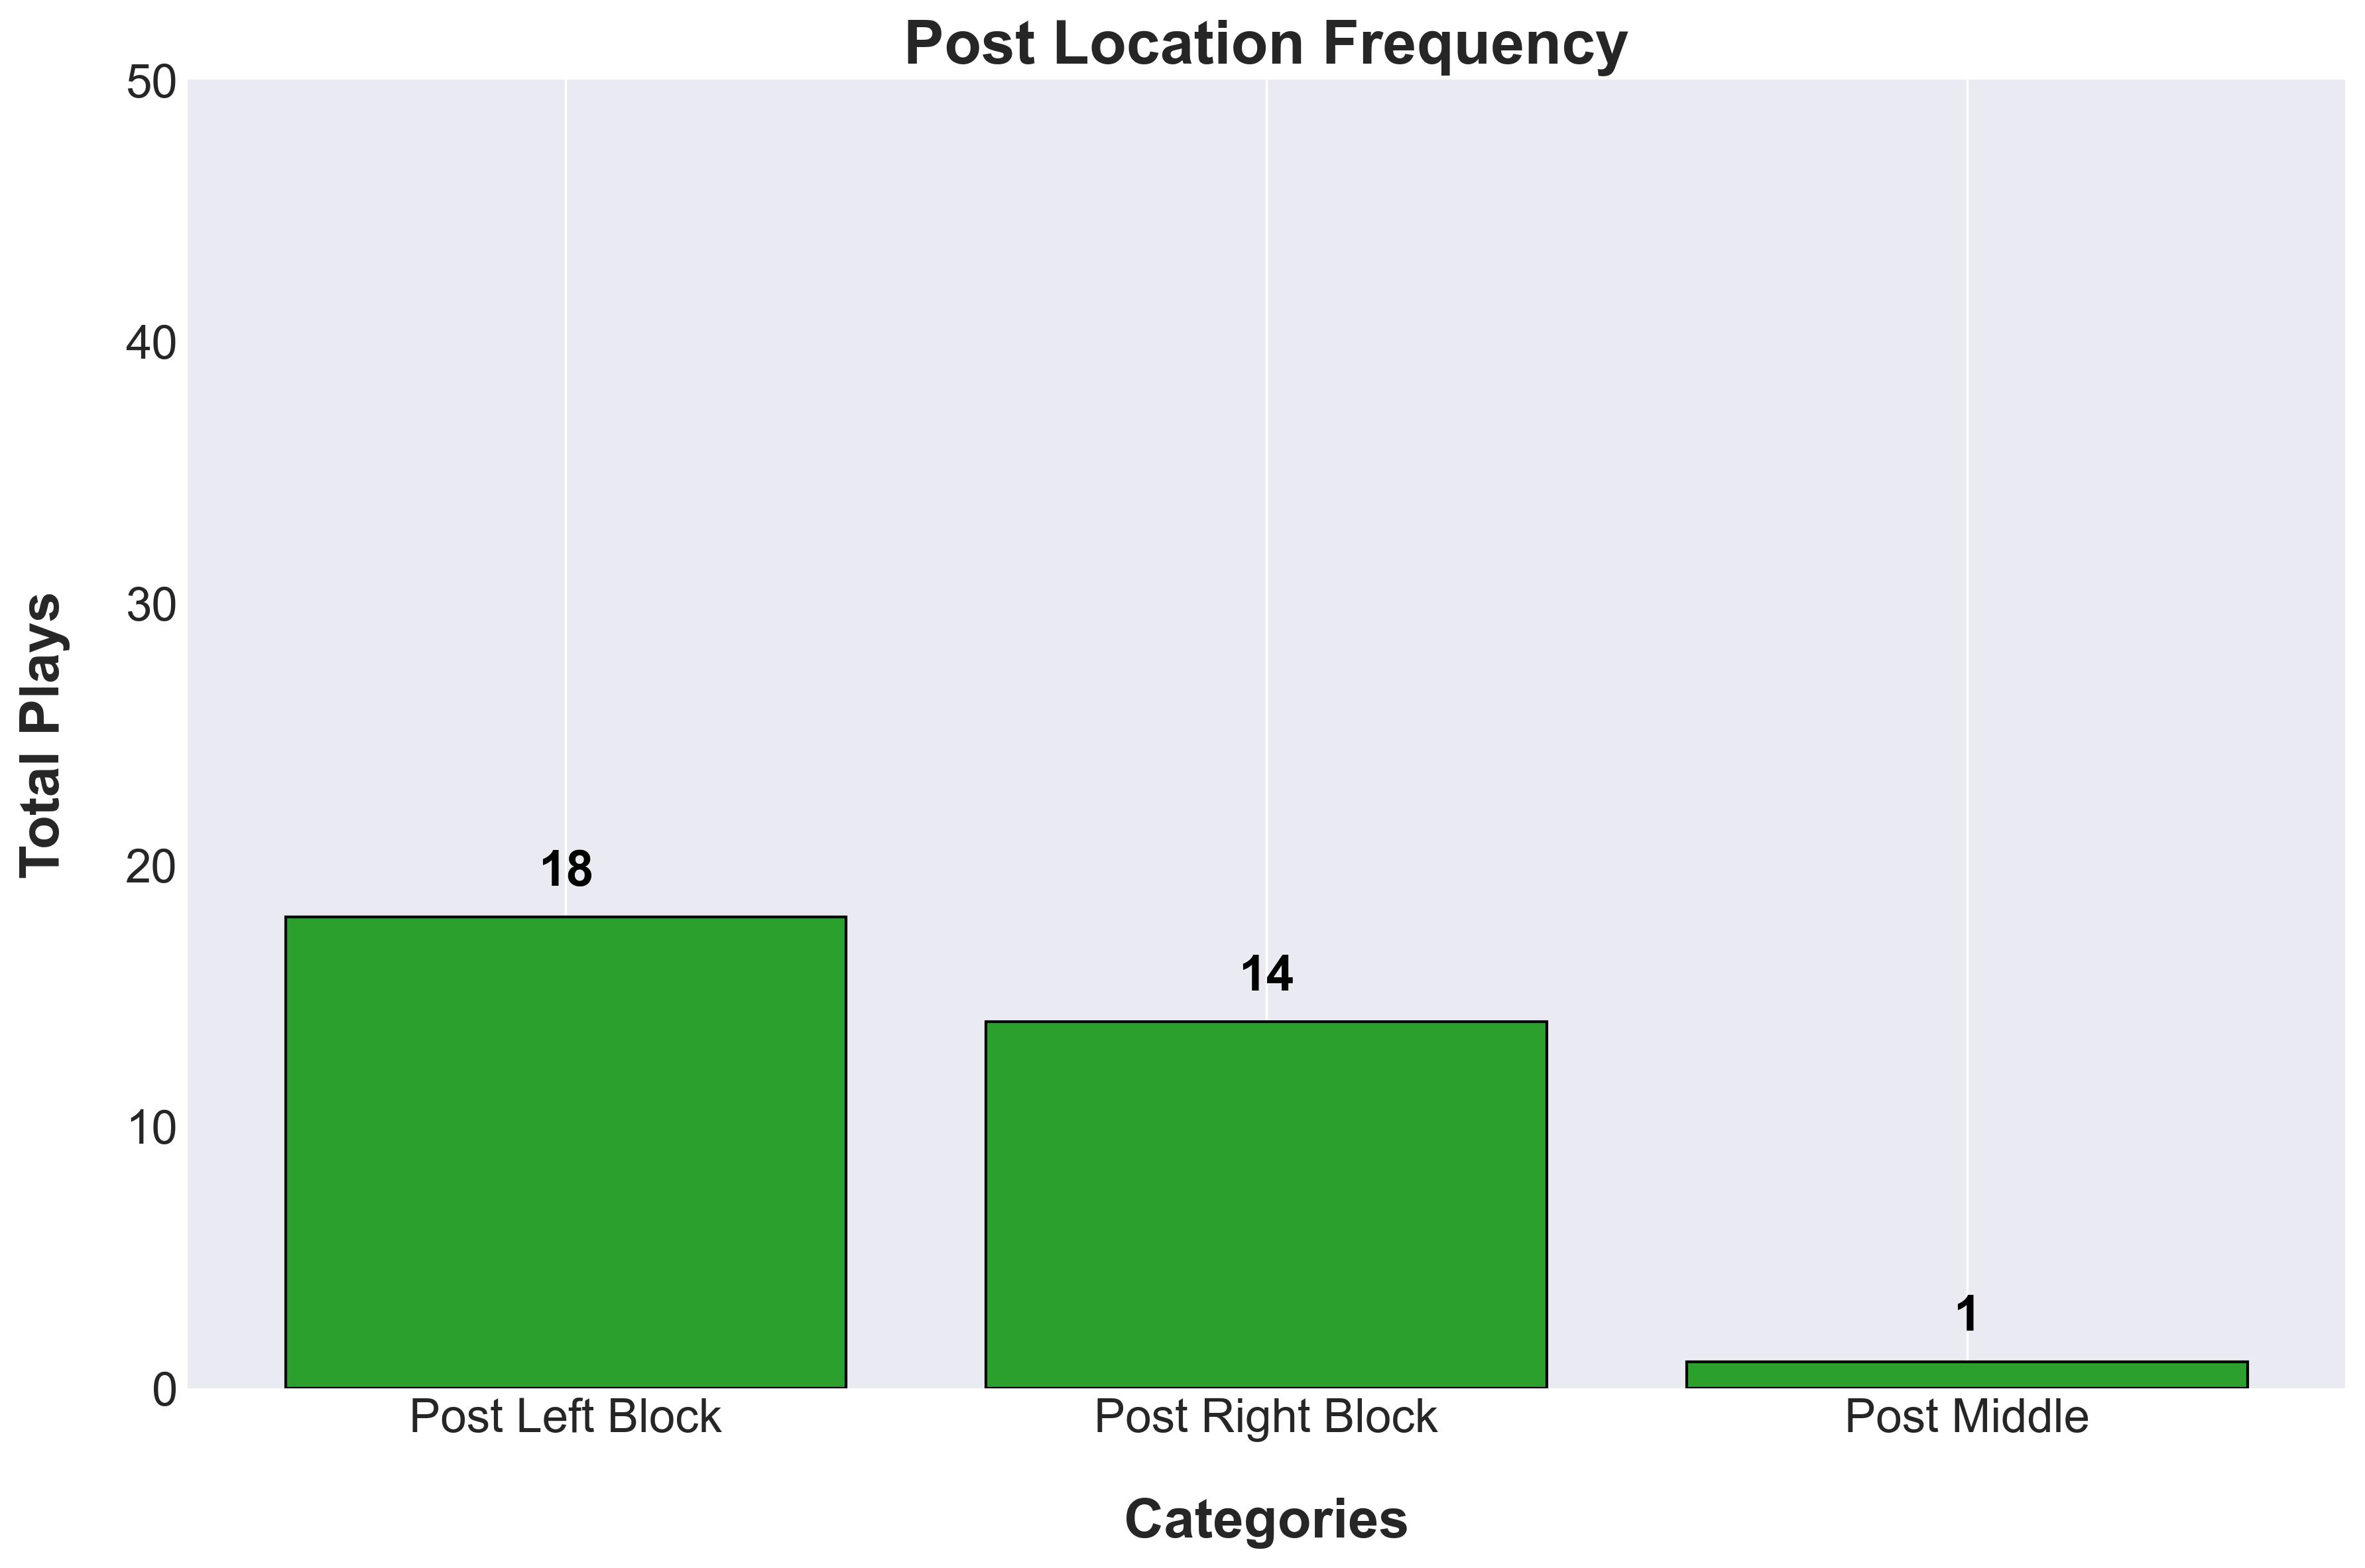
\includegraphics[width=\textwidth, height=.14\textheight]{images/Post_Location_Freq.png} % Adjust the width of the image to fit
    \end{minipage}
\end{table}

\vspace{-1em} % Add vertical space before the line (optional)
%\hrule height 1pt width 1\textwidth % Adjust height and width
\vspace{-1em} % Add vertical space after the line (optional)

% Post Shot Type Statistics
\begin{table}[H]
    \raisebox{3.5em}{ % Adjust this value to shift the tables vertically
    \begin{minipage}[t]{0.6\textwidth} % Left side (table) takes 85% of the width
        \flushleft
        \centering % Centering the title and the table
        \text{Post Shot Type Statistics} % Title above the table in bold
        \vskip .25em % Adds vertical space between title and table
        \scalebox{.6}{ % Scale the entire table down by half
            \renewcommand{\arraystretch}{1.4} % Adjust the number to increase or decrease row spacing
            \begin{tabular}{
            >{\centering\arraybackslash}p{2.75cm} 
            >{\centering\arraybackslash}p{.75cm} 
            >{\centering\arraybackslash}p{.75cm} 
            >{\centering\arraybackslash}p{.75cm} 
            >{\centering\arraybackslash}p{.75cm}
            >{\centering\arraybackslash}p{.75cm} 
            >{\centering\arraybackslash}p{.75cm}
            >{\centering\arraybackslash}p{.75cm}
            >{\centering\arraybackslash}p{.75cm} 
            >{\centering\arraybackslash}p{.75cm}}% Adjust column widths
            \toprule
            {\scriptsize \textbf{Shot Type}} &
            {\scriptsize \textbf{Plays}} &
            {\scriptsize \textbf{2PA}} & 
            {\scriptsize \textbf{2PM}} & 
            {\scriptsize \textbf{2P\%}} & 
            {\scriptsize \textbf{MiA}} & 
            {\scriptsize \textbf{MiM}} &
            {\scriptsize \textbf{Mi\%}} &
            {\scriptsize \textbf{TO}} &
            {\scriptsize \textbf{Foul}} \\
            \midrule
            
                
            
                
            
                
            
                
            
                
            
                
            
                
            
                
            
                
            
                
            
                
            
                
                    Left Shoulder & 19 &
                    16 & 5 &
                    31.25 &
                    0 & 0 &
                    - &
                    1 & 2 \\
                
            
                
                    Right Shoulder & 7 &
                    4 & 0 &
                    0.0 &
                    0 & 0 &
                    - &
                    3 & 0 \\
                
            
                
                    Face-up & 7 &
                    6 & 1 &
                    16.67 &
                    0 & 0 &
                    - &
                    1 & 0 \\
                
            
                
            
                
            
                
            
                
            
                
            
                
            
                
            
                
            
                
            


            \bottomrule
        \end{tabular}
        } % End of \scalebox
    \end{minipage}
    } % End of raisebox, closing the adjustment
    \hfill
    \begin{minipage}[c]{0.35\textwidth} % Right side (image) takes 10% of the width
        \flushright
        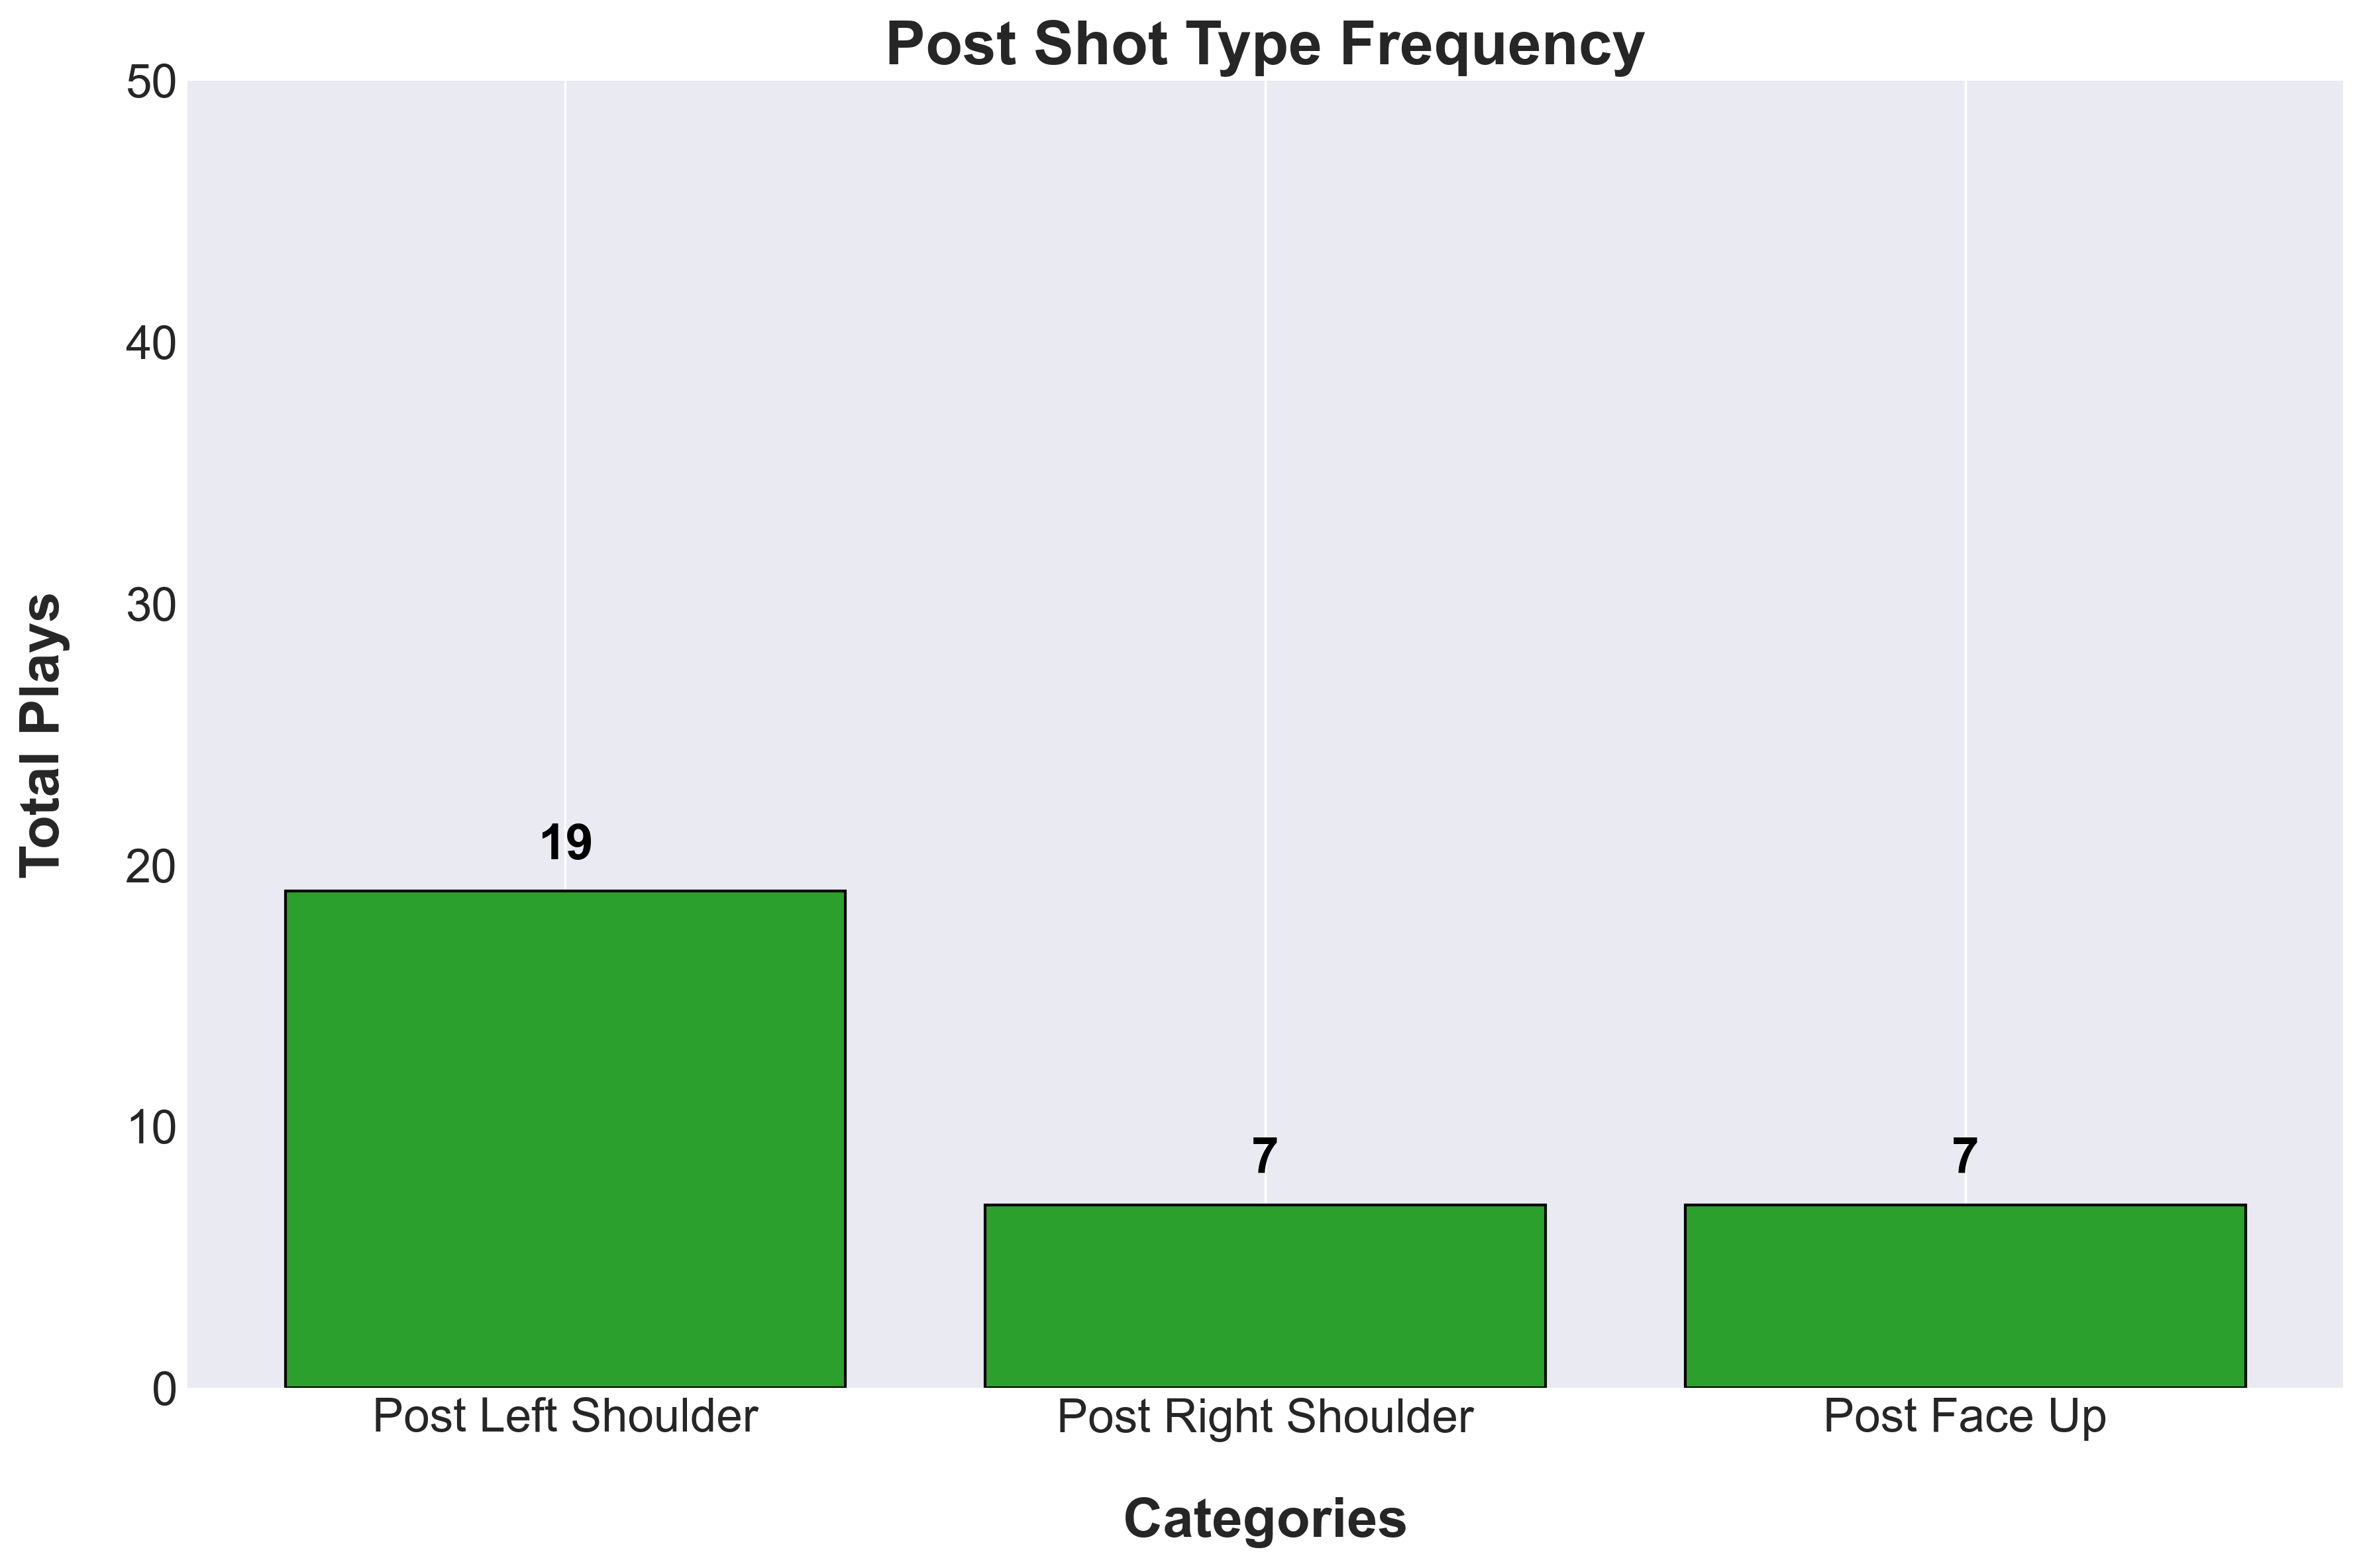
\includegraphics[width=\textwidth, height=.14\textheight]{images/Post_ShotType_Freq.png} % Adjust the width of the image to fit
    \end{minipage}
    
\end{table}

\vspace{-1em} % Add vertical space before the line (optional)
%\hrule height 1pt width 1\textwidth % Adjust height and width
\vspace{-1em} % Add vertical space after the line (optional)

% Post Stats for Combination of Location and Shot Type Stats
\begin{table}[H]
    \raisebox{6em}{ % Adjust this value to shift the tables vertically
    \begin{minipage}[t]{0.6\textwidth} % Left side (table) takes 85% of the width
        \flushleft
        \centering % Centering the title and the table
        \text{Post Combination Statistics} % Title above the table in bold
        \vskip .25em % Adds vertical space between title and table
        \scalebox{.6}{ % Scale the entire table down by half
            \renewcommand{\arraystretch}{1.4} % Adjust the number to increase or decrease row spacing
            \begin{tabular}{
            >{\centering\arraybackslash}p{5.5cm} 
            >{\centering\arraybackslash}p{.75cm} 
            >{\centering\arraybackslash}p{.75cm} 
            >{\centering\arraybackslash}p{.75cm} 
            >{\centering\arraybackslash}p{.75cm}
            >{\centering\arraybackslash}p{.75cm} 
            >{\centering\arraybackslash}p{.75cm} 
            >{\centering\arraybackslash}p{.75cm}
            >{\centering\arraybackslash}p{.75cm} 
            >{\centering\arraybackslash}p{.75cm}}% Adjust column widths
            \toprule
            {\scriptsize \textbf{PlayType}} &
            {\scriptsize \textbf{Plays}} &
            {\scriptsize \textbf{2PA}} & 
            {\scriptsize \textbf{2PM}} & 
            {\scriptsize \textbf{2P\%}} & 
            {\scriptsize \textbf{MiA}} & 
            {\scriptsize \textbf{MiM}} &
            {\scriptsize \textbf{Mi\%}} &
            {\scriptsize \textbf{TO}} &
            {\scriptsize \textbf{Foul}} \\
            \midrule
            
                
            
                
            
                
            
                
            
                
            
                
            
                
            
                
            
                
            
                
            
                
            
                
            
                
            
                
            
                
                    Left Block - Face Up & 2 &
                    2 & 0 &
                    0.0 &
                    0 & 0 &
                    - &
                    0 & 0 \\
                
            
                
                    Left Block - Left Shoulder & 12 &
                    10 & 3 &
                    30.0 &
                    0 & 0 &
                    - &
                    1 & 1 \\
                
            
                
                    Left Block - Right Shoulder & 4 &
                    2 & 0 &
                    0.0 &
                    0 & 0 &
                    - &
                    2 & 0 \\
                
            
                
                    Right Block - Face Up & 4 & 
                    4 & 1 &
                    25.0 &
                    0 & 0 &
                    - &
                    0 & 0 \\
                
            
                
                    Right Block - Left Shoulder & 7 & 
                    6 & 2 &
                    33.33 &
                    0 & 0 &
                    - &
                    0 & 1 \\
                
            
                
                    Right Block - Right Shoulder & 3 & 
                    2 & 0 &
                    0.0 &
                    0 & 0 &
                    - &
                    1 & 0 \\
                
            
                
                    Middle - Face Up & 1 &
                    0 & 0 &
                    - &
                    0 & 0 &
                    - &
                    1 & 0 \\
                
            
                
            
                
            


            \bottomrule
        \end{tabular}
        } % End of \scalebox
    \end{minipage}
    } % End of raisebox, closing the adjustment
    \hfill % This adds some flexible space between the table and the image
    \begin{minipage}[c]{0.35\textwidth} % Right side (image) takes 10% of the width
        \flushright
        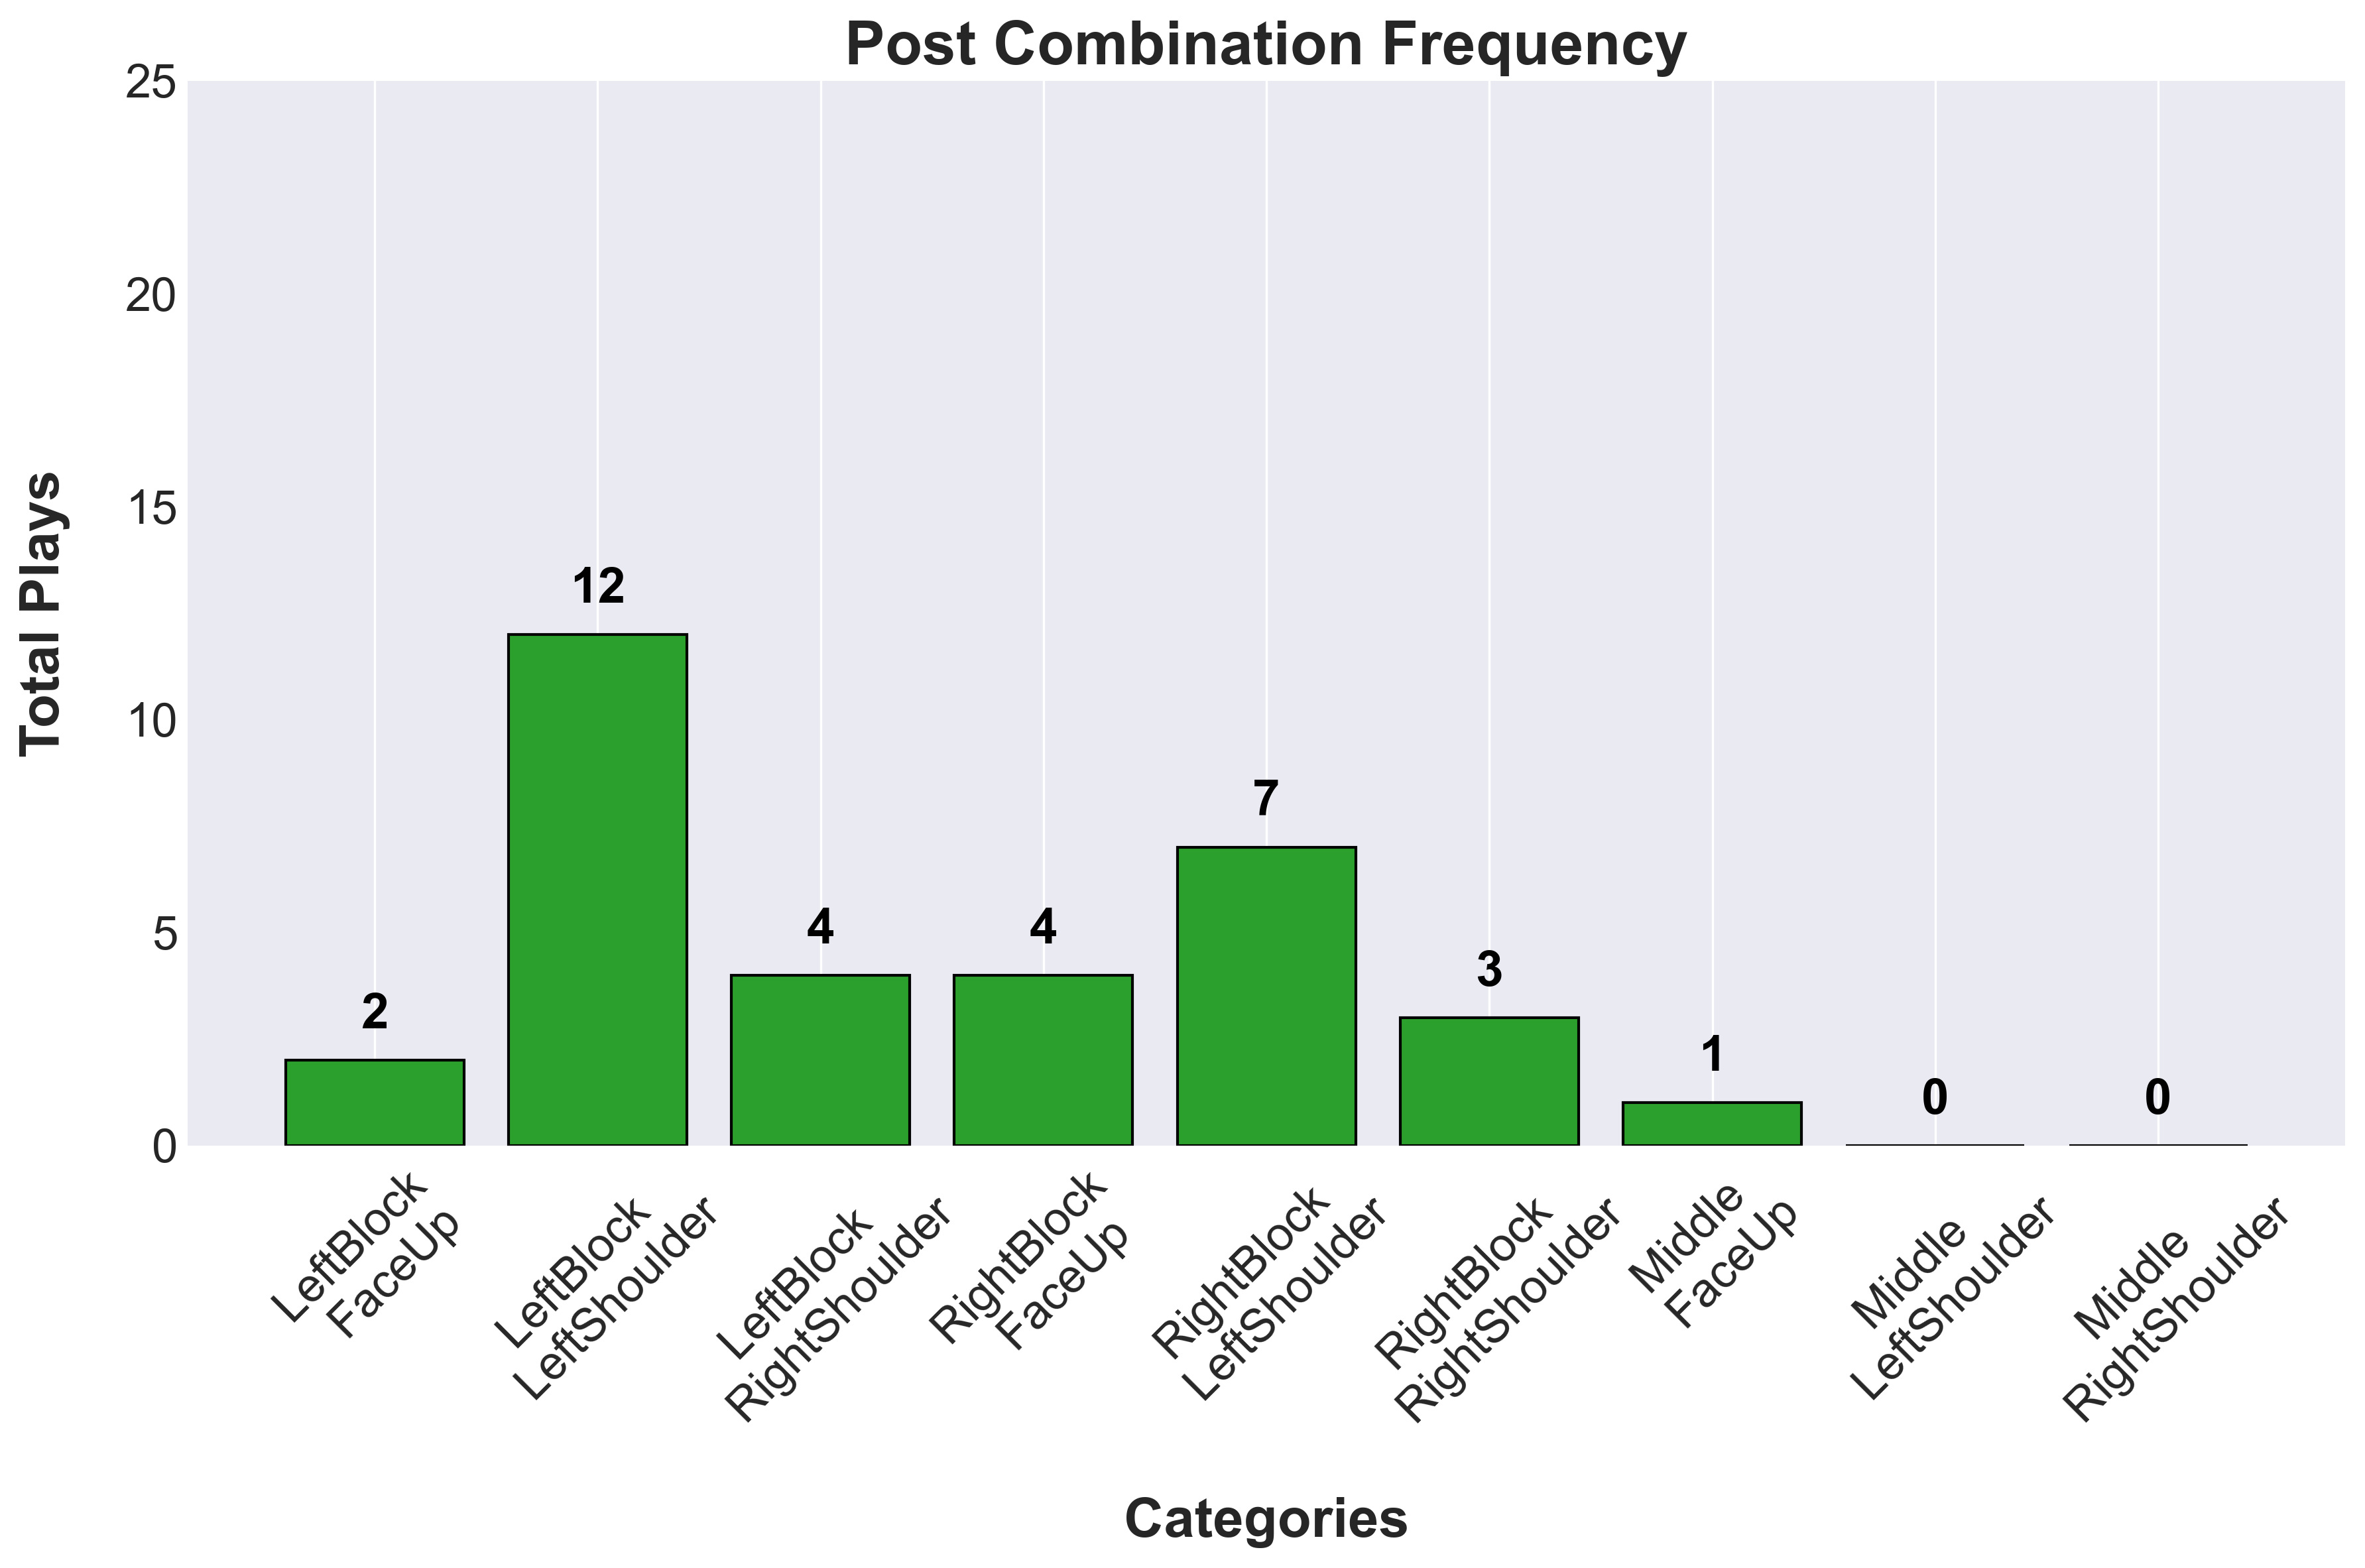
\includegraphics[width=\textwidth, height=.14\textheight]{images/Post_Combination_Freq.png} % Adjust the width of the image to fit
    \end{minipage}
\end{table}

\vspace{0em} % Add vertical space before the line (optional)
\hrule height 1pt width 1\textwidth % Adjust height and width
\vspace{1em} % Add vertical space after the line (optional)

\subsubsection{Post Passer Statistics}

\vspace{-1em} % Add vertical space before the line (optional)

% Total Post Passer Statistics
\begin{table}[H]
    \raisebox{2.5em}{ % Adjust this value to shift the tables vertically
    \begin{minipage}[t]{0.6\textwidth} % Left side (table) takes 85% of the width
        %\flushright
        \centering % Centering the title and the table
        \text{Total Post Passer Statistics} % Title above the table in bold
        \vskip .25em % Adds vertical space between title and table
        \scalebox{.85}{ % Scale the entire table down by half
            \scriptsize % Reduce the font size
            \begin{tabular}{
            >{\centering\arraybackslash}p{.75cm} 
            >{\centering\arraybackslash}p{.5cm} 
            >{\centering\arraybackslash}p{.5cm} 
            >{\centering\arraybackslash}p{.5cm}
            >{\centering\arraybackslash}p{.5cm} 
            >{\centering\arraybackslash}p{.5cm} 
            >{\centering\arraybackslash}p{.5cm} 
            >{\centering\arraybackslash}p{.5cm}
            >{\centering\arraybackslash}p{.5cm} 
            >{\centering\arraybackslash}p{.5cm}
            >{\centering\arraybackslash}p{.5cm} 
            >{\centering\arraybackslash}p{.5cm}}% Adjust column widths
            \toprule
            \textbf{Plays} &
            \textbf{3PA} &
            \textbf{3PM} &
            \textbf{3P\%} & 
            \textbf{2PA} & 
            \textbf{2PM} & 
            \textbf{2P\%} & 
            \textbf{MiA} & 
            \textbf{MiM} &
            \textbf{Mi\%} &
            \textbf{TO} &
            \textbf{Foul} \\
            \midrule
            
                
            
                
                    4 & 3 & 1 &
                    33.33 & 
                    1 & 0 &
                    0.0 &
                    0 & 0 &
                    - &
                    0 & 0 \\
                
            
                
            
                
            
                
            
                
            
                
            
                
            
                
            
                
            
                
            
                
            
                
            
                
            
                
            
                
            
                
            
                
            
                
            
                
            
                
            
                
            
                
            


            \bottomrule
            \end{tabular}
        }
    \end{minipage}
    }
    \hfill % This adds some flexible space between the table and the image
    \begin{minipage}[c]{0.35\textwidth} % Right side (image) takes 10% of the width
        \flushright
        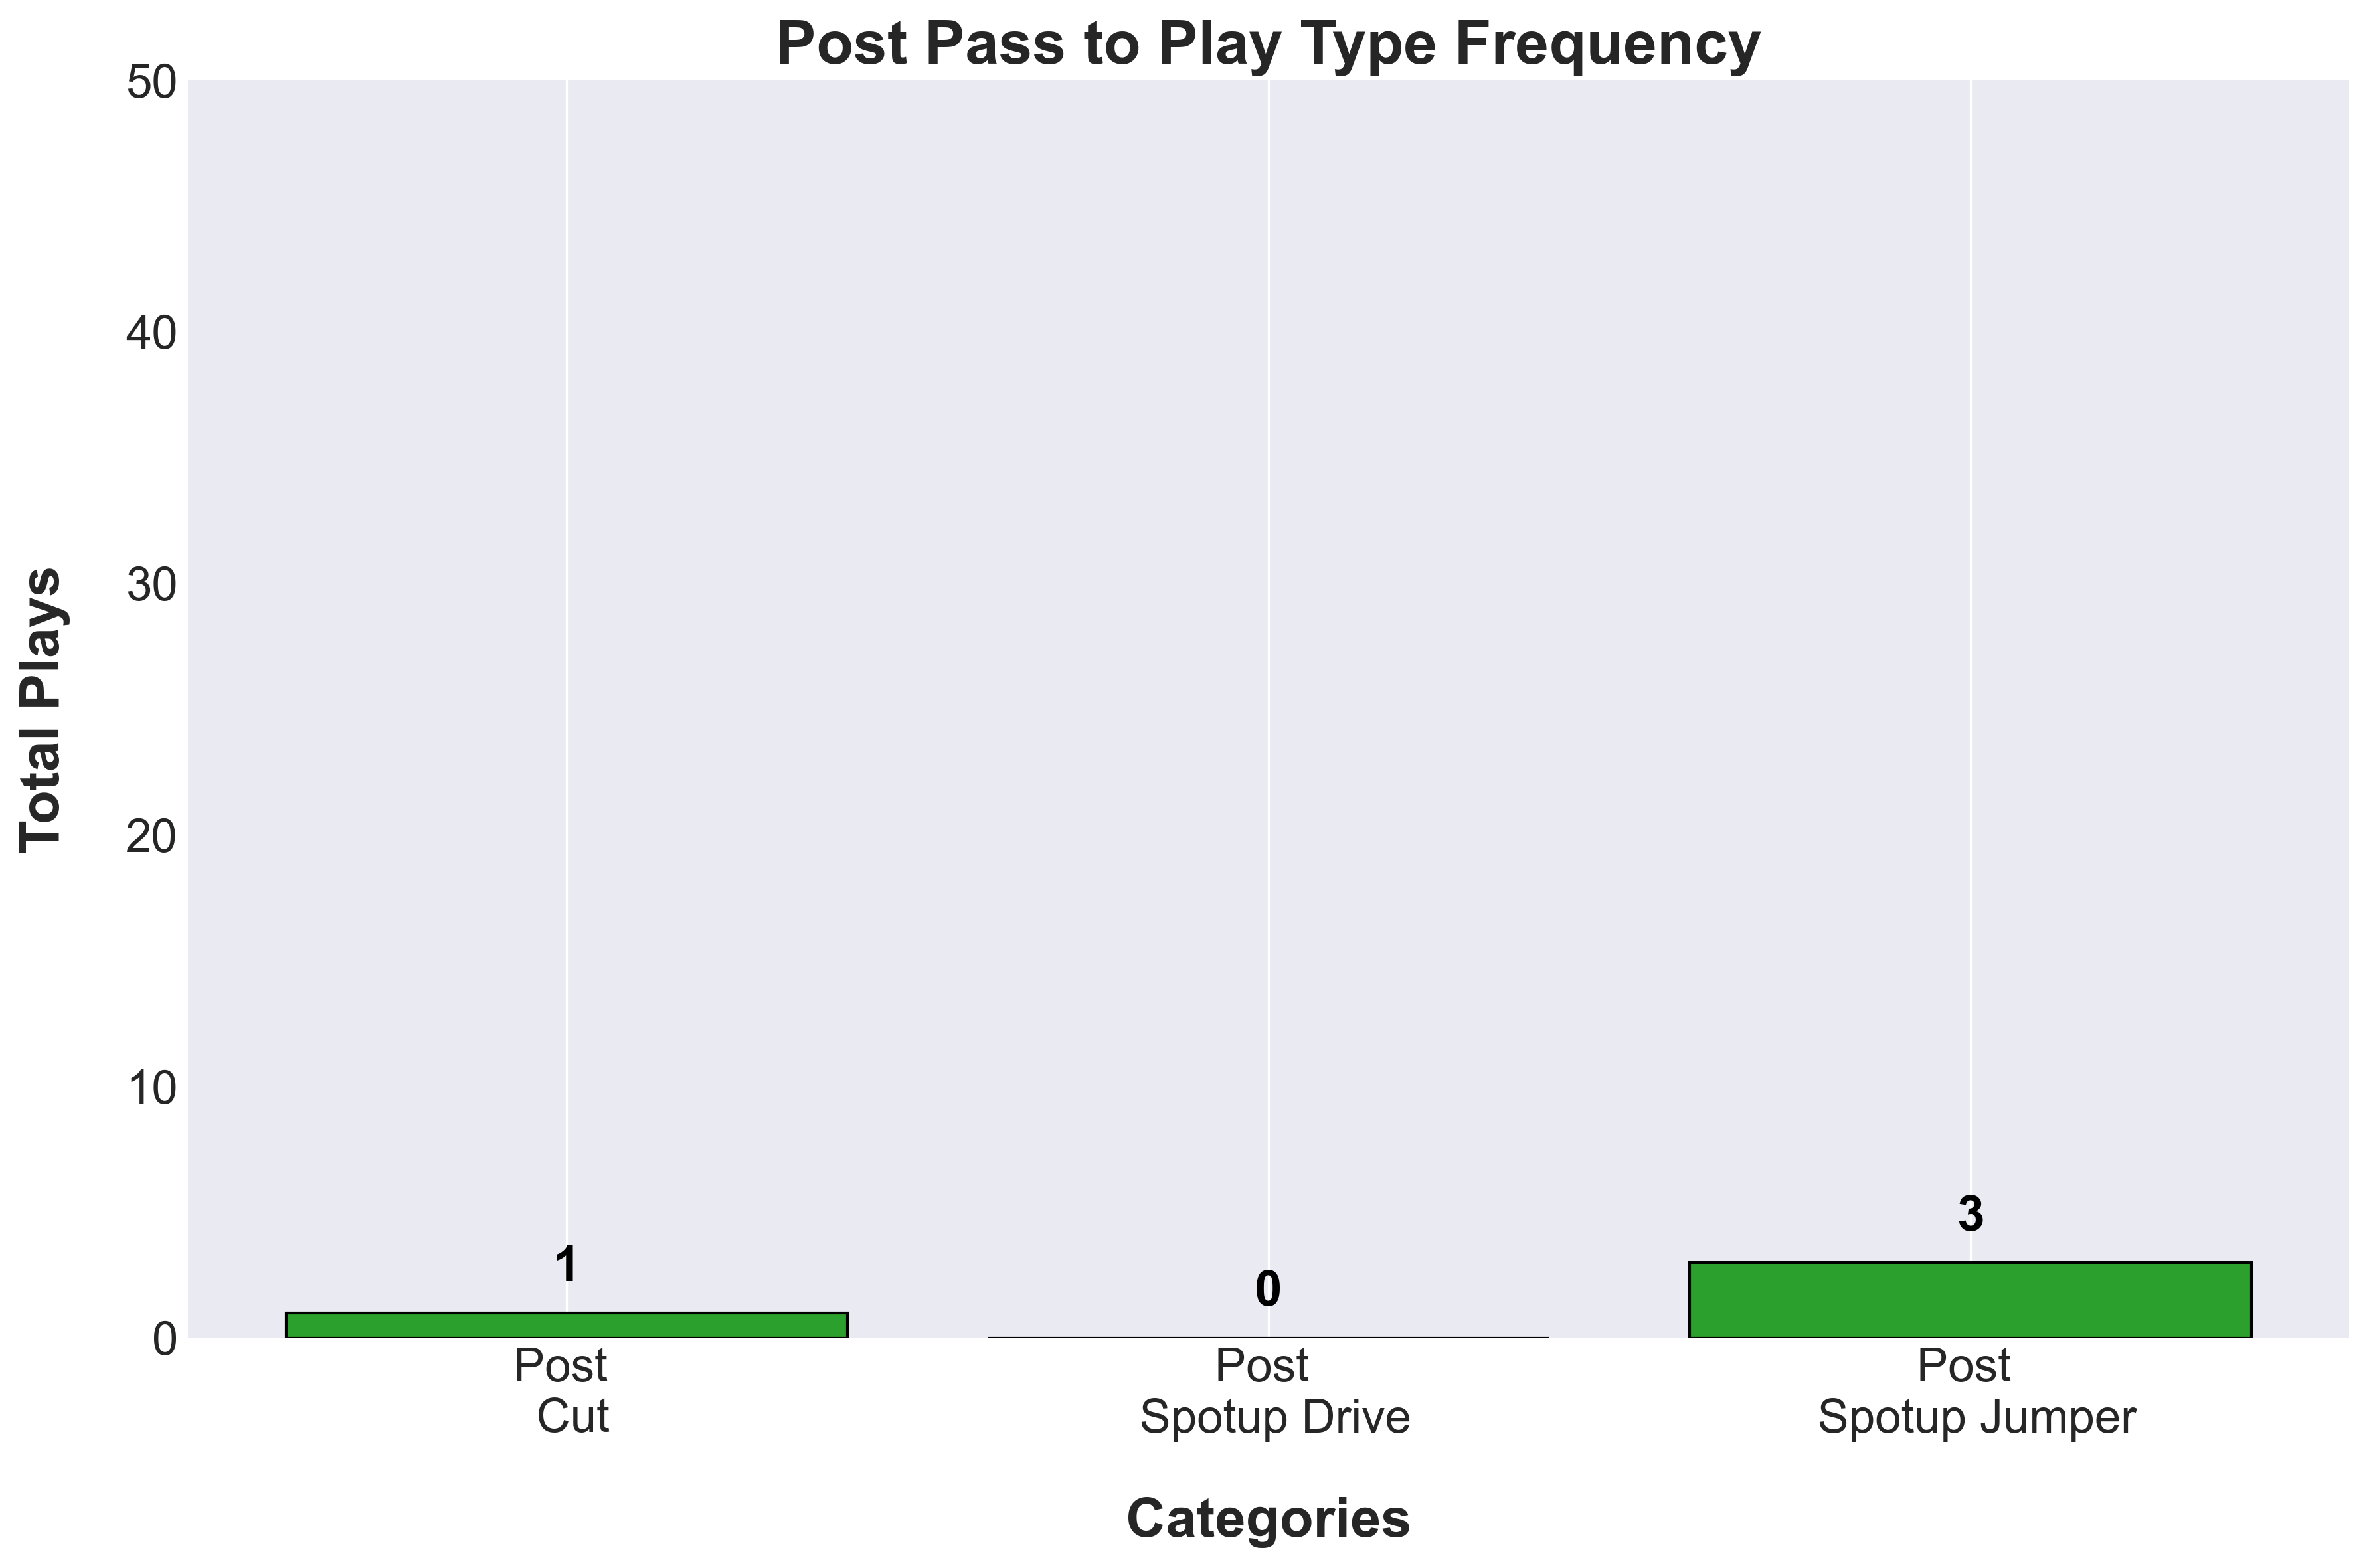
\includegraphics[width=\textwidth, height=.14\textheight]{images/Post_PassPlayType_Freq.png} % Adjust the width of the image to fit
    \end{minipage}
\end{table}

\vspace{-1em} % Add vertical space before the line (optional)
\vspace{1em} % Add vertical space after the line (optional)

% Post -> Cut Secondary Player Stats
\begin{table}[H]
    \raisebox{3em}{ % Adjust this value to shift the tables vertically
    \begin{minipage}[t]{0.6\textwidth} % Left side (table) takes 85% of the width
        \flushleft
        \centering % Centering the title and the table
        \text{Post - Cut Player Statistics} % Title above the table in bold
        \vskip .25em % Adds vertical space between title and table
        \scalebox{.55}{ % Scale the entire table down by half
            \renewcommand{\arraystretch}{1.4} % Adjust the number to increase or decrease row spacing
            \begin{tabular}{
            >{\centering\arraybackslash}p{3cm} 
            >{\centering\arraybackslash}p{.75cm} 
            >{\centering\arraybackslash}p{.75cm} 
            >{\centering\arraybackslash}p{.75cm} 
            >{\centering\arraybackslash}p{.75cm}
            >{\centering\arraybackslash}p{.75cm} 
            >{\centering\arraybackslash}p{.75cm} 
            >{\centering\arraybackslash}p{.75cm} 
            >{\centering\arraybackslash}p{.75cm} 
            >{\centering\arraybackslash}p{.75cm}}% Adjust column widths
            \toprule
            {\scriptsize \textbf{Player}} &
            {\scriptsize \textbf{Plays}} &
            {\scriptsize \textbf{2PA}} & 
            {\scriptsize \textbf{2PM}} & 
            {\scriptsize \textbf{2P\%}} & 
            {\scriptsize \textbf{MiA}} & 
            {\scriptsize \textbf{MiM}} &
            {\scriptsize \textbf{Mi\%}} &
            {\scriptsize \textbf{TO}} &
            {\scriptsize \textbf{Foul}} \\
            \midrule
            
                
            
                
            
                
                    
                        Brock Bowen & 
                        1 & 
                        1 & 
                        0 & 
                        0.0 & 
                        0 & 
                        0 & 
                        - & 
                        0 & 
                        0 \\
                    
                
            
                
            
                
            
                
            
                
            
                
            
                
            
                
            
                
            
                
            
                
            
                
            
                
            
                
            
                
            
                
            
                
            
                
            
                
            
                
            
                
            

            \bottomrule
        \end{tabular}
        } % End of \scalebox
    \end{minipage}
    } % End of raisebox, closing the adjustment
    \hfill % This adds some flexible space between the table and the image
    \begin{minipage}[c]{0.35\textwidth} % Right side (image) takes 10% of the width
        \flushright
        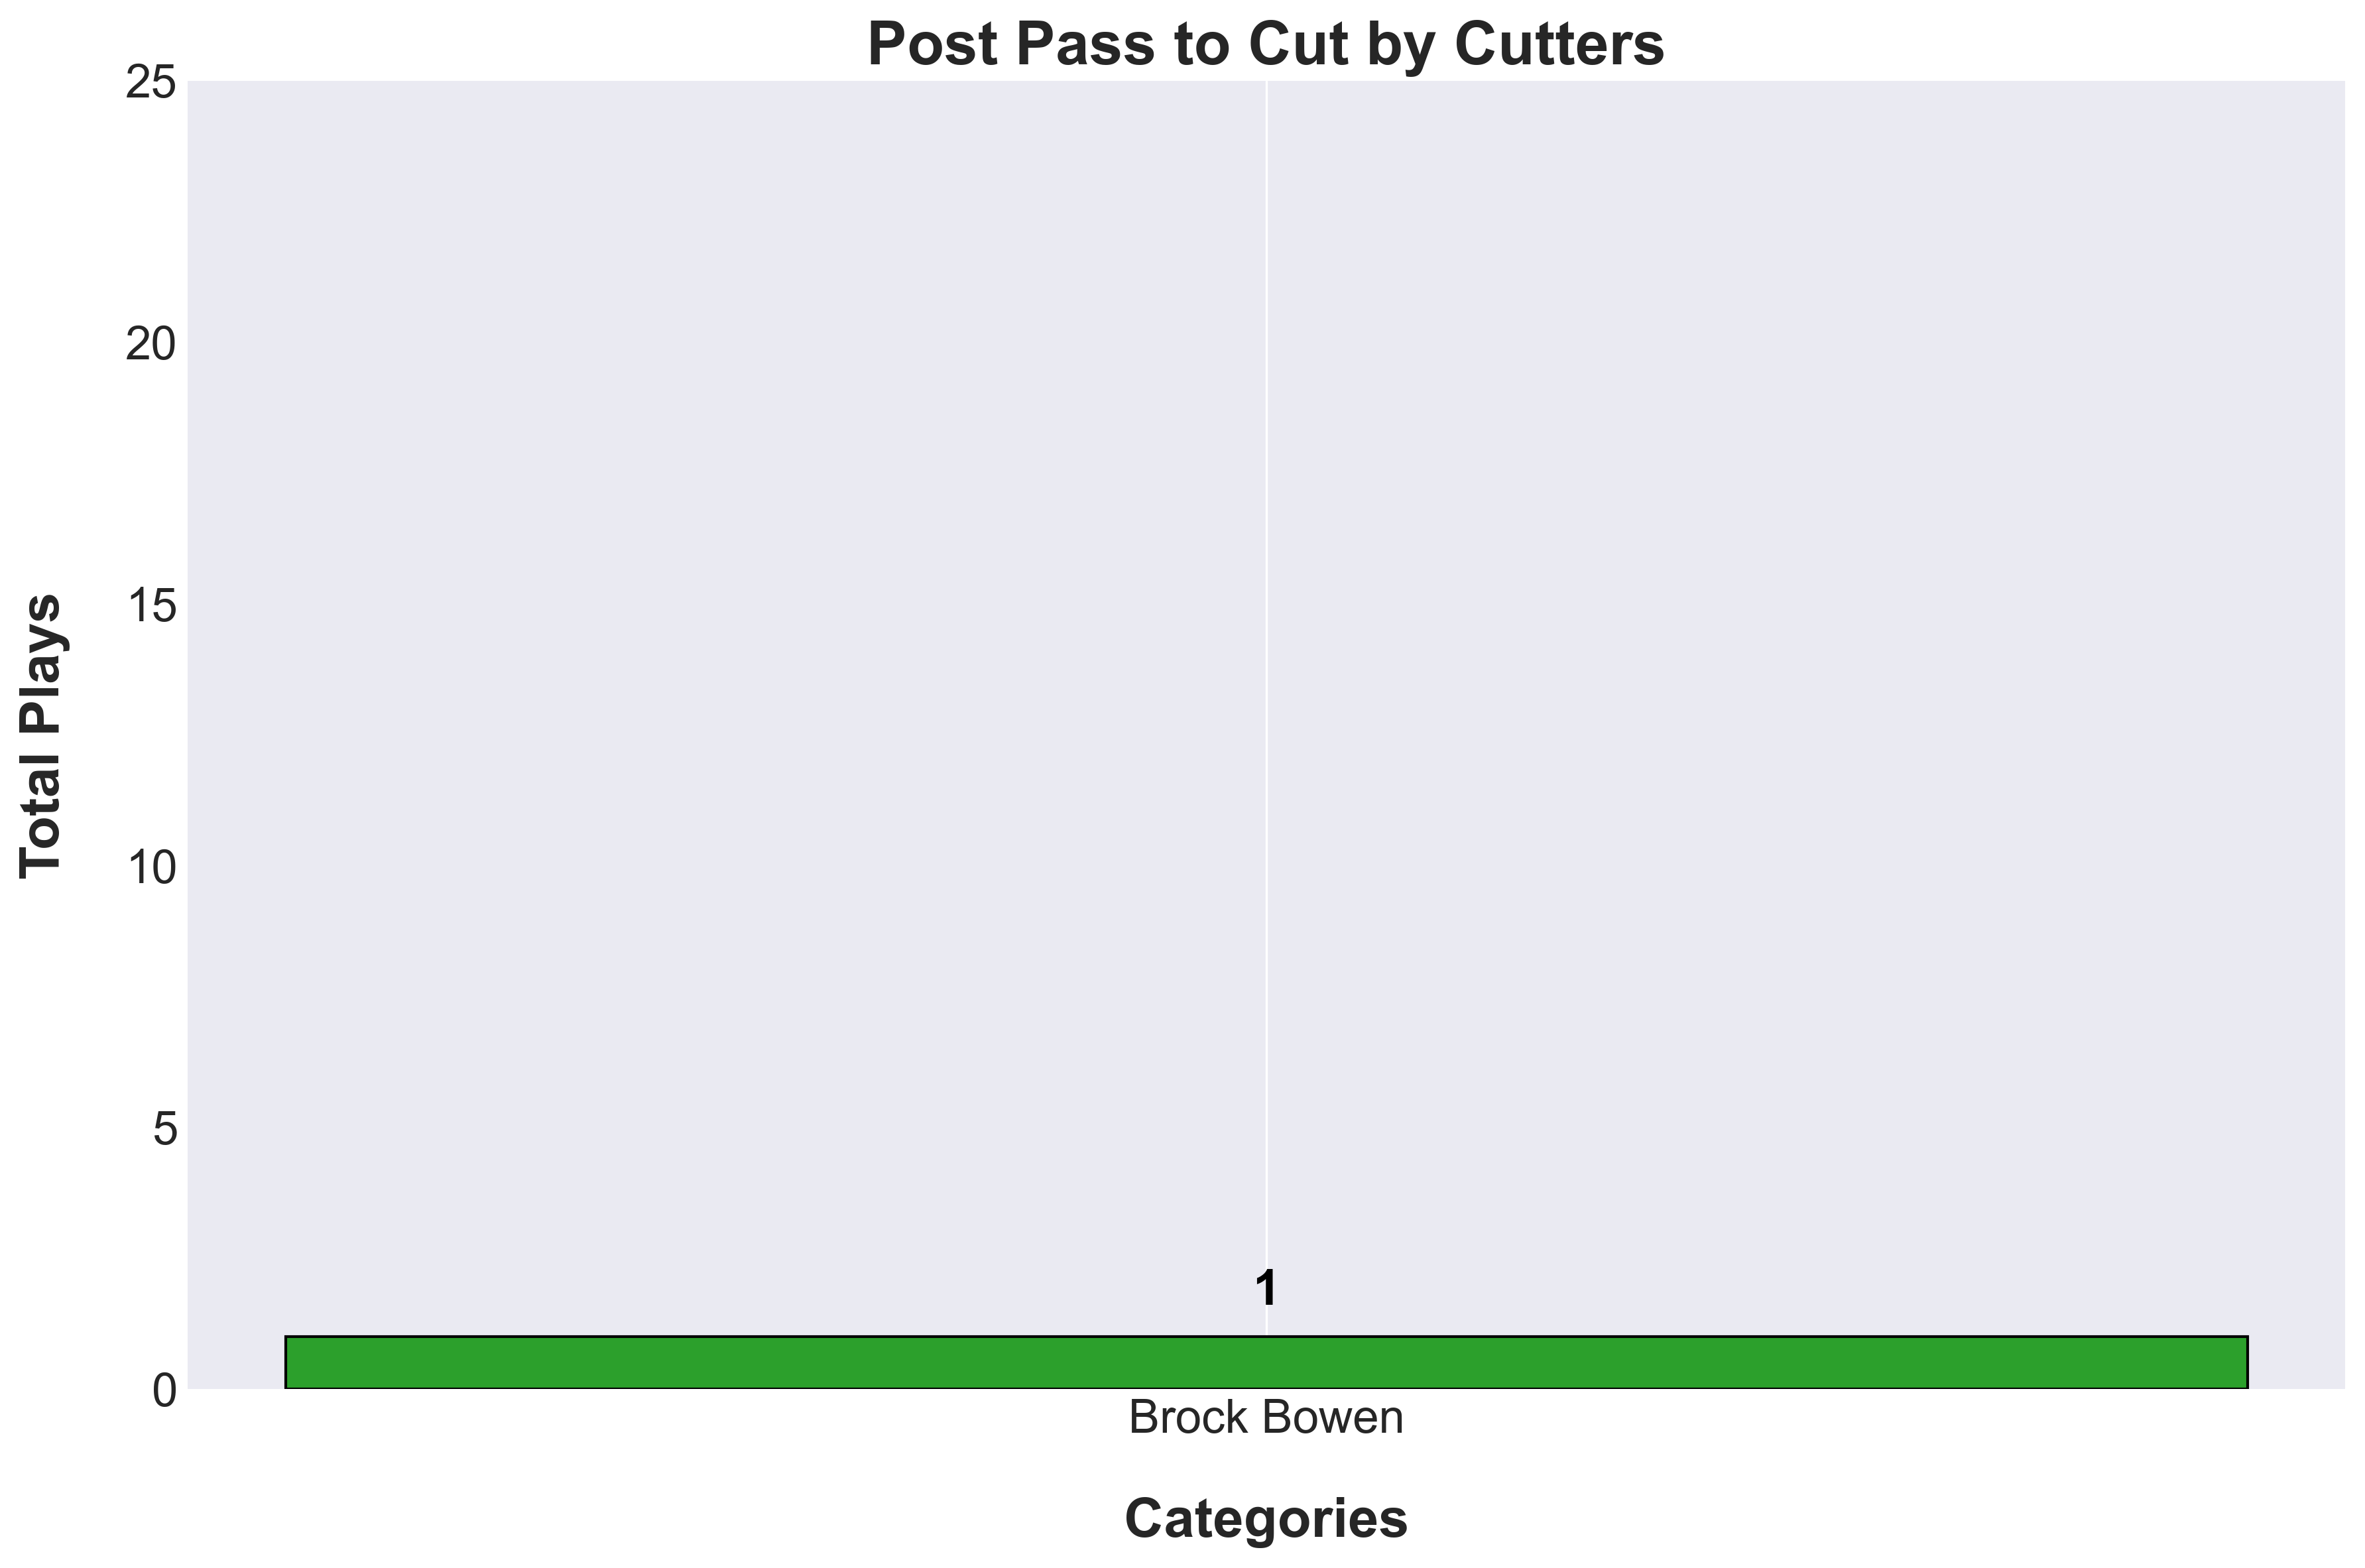
\includegraphics[width=\textwidth, height=.14\textheight]{images/Post_PassCutsPlayer_Freq.png} % Adjust the width of the image to fit
    \end{minipage}
\end{table}

\vspace{-1em} % Add vertical space before the line (optional)
\vspace{-1em} % Add vertical space after the line (optional)

% Post -> Spot Up Drives Secondary Player Stats
\begin{table}[H]
    \raisebox{3em}{ % Adjust this value to shift the tables vertically
    \begin{minipage}[t]{0.6\textwidth} % Left side (table) takes 85% of the width
        \flushleft
        \centering % Centering the title and the table
        \text{Post - Spot Up Drives Player Statistics} % Title above the table in bold
        \vskip .25em % Adds vertical space between title and table
        \scalebox{.55}{ % Scale the entire table down by half
            \renewcommand{\arraystretch}{1.4} % Adjust the number to increase or decrease row spacing
            \begin{tabular}{
            >{\centering\arraybackslash}p{3cm} 
            >{\centering\arraybackslash}p{.75cm} 
            >{\centering\arraybackslash}p{.75cm} 
            >{\centering\arraybackslash}p{.75cm} 
            >{\centering\arraybackslash}p{.75cm}
            >{\centering\arraybackslash}p{.75cm} 
            >{\centering\arraybackslash}p{.75cm} 
            >{\centering\arraybackslash}p{.75cm} 
            >{\centering\arraybackslash}p{.75cm}
            >{\centering\arraybackslash}p{.75cm} 
            >{\centering\arraybackslash}p{.75cm}
            >{\centering\arraybackslash}p{.75cm} 
            >{\centering\arraybackslash}p{.75cm}}% Adjust column widths
            \toprule
            {\scriptsize \textbf{Player}} &
            {\scriptsize \textbf{Plays}} &
            {\scriptsize \textbf{3PA}} &
            {\scriptsize \textbf{3PM}} &
            {\scriptsize \textbf{3P\%}} & 
            {\scriptsize \textbf{2PA}} & 
            {\scriptsize \textbf{2PM}} & 
            {\scriptsize \textbf{2P\%}} & 
            {\scriptsize \textbf{MiA}} & 
            {\scriptsize \textbf{MiM}} &
            {\scriptsize \textbf{Mi\%}} &
            {\scriptsize \textbf{TO}} &
            {\scriptsize \textbf{Foul}} \\
            \midrule
            
                
            
                
            
                
            
                
                    
                
            
                
            
                
            
                
            
                
            
                
            
                
            
                
            
                
            
                
            
                
            
                
            
                
            
                
            
                
            
                
            
                
            
                
            
                
            
                
            

            \bottomrule
        \end{tabular}
        } % End of \scalebox
    \end{minipage}
    } % End of raisebox, closing the adjustment
    \hfill % This adds some flexible space between the table and the image
    \begin{minipage}[c]{0.35\textwidth} % Right side (image) takes 10% of the width
        \flushright
        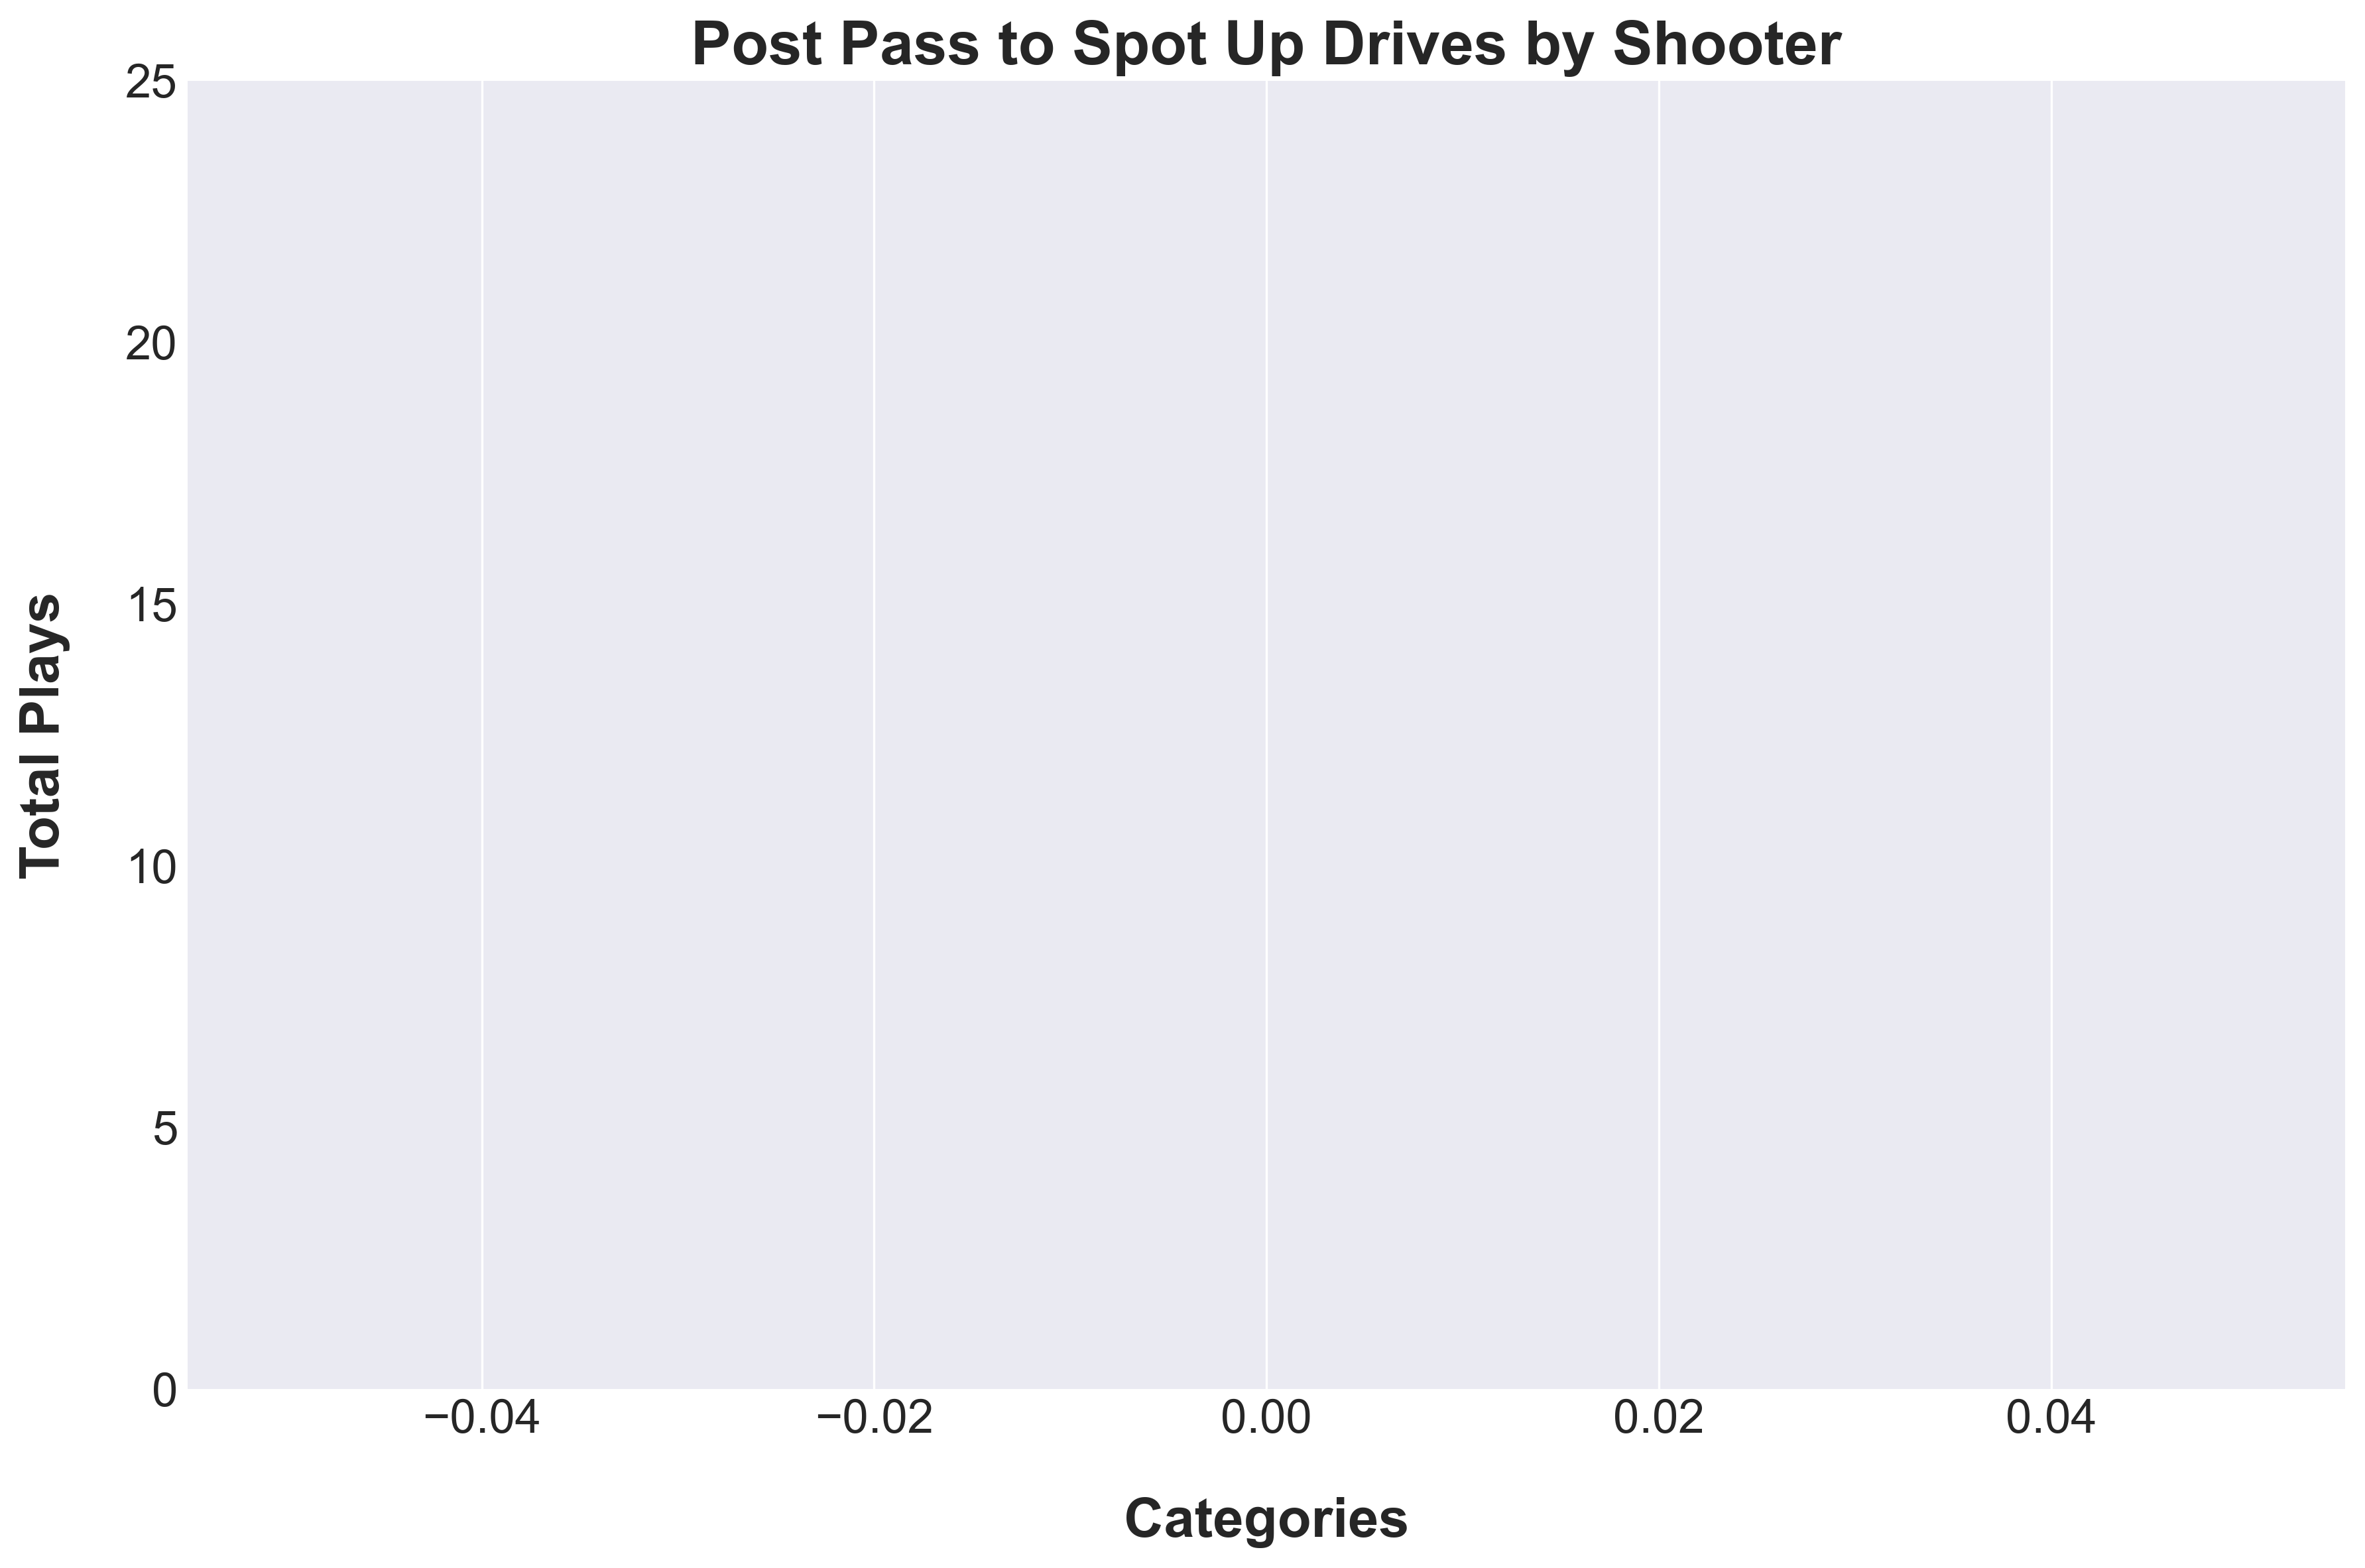
\includegraphics[width=\textwidth, height=.14\textheight]{images/Post_PassDrivesPlayer_Freq.png} % Adjust the width of the image to fit
    \end{minipage}
\end{table}

\vspace{-1em} % Add vertical space before the line (optional)
\vspace{-1em} % Add vertical space after the line (optional)

% Post -> Spot Up Jumpers Secondary Player Stats
\begin{table}[H]
    \raisebox{3em}{ % Adjust this value to shift the tables vertically
    \begin{minipage}[t]{0.6\textwidth} % Left side (table) takes 85% of the width
        \flushleft
        \centering % Centering the title and the table
        \text{Post - Spot Up Jumpers Player Statistics} % Title above the table in bold
        \vskip .25em % Adds vertical space between title and table
        \scalebox{.55}{ % Scale the entire table down by half
            \renewcommand{\arraystretch}{1.4} % Adjust the number to increase or decrease row spacing
            \begin{tabular}{
            >{\centering\arraybackslash}p{3cm} 
            >{\centering\arraybackslash}p{.75cm} 
            >{\centering\arraybackslash}p{.75cm} 
            >{\centering\arraybackslash}p{.75cm} 
            >{\centering\arraybackslash}p{.75cm} 
            >{\centering\arraybackslash}p{.75cm}
            >{\centering\arraybackslash}p{.75cm} 
            >{\centering\arraybackslash}p{.75cm}
            >{\centering\arraybackslash}p{.75cm} 
            >{\centering\arraybackslash}p{.75cm}}% Adjust column widths
            \toprule
            {\scriptsize \textbf{Player}} &
            {\scriptsize \textbf{Plays}} &
            {\scriptsize \textbf{3PA}} &
            {\scriptsize \textbf{3PM}} &
            {\scriptsize \textbf{3P\%}} & 
            {\scriptsize \textbf{MiA}} & 
            {\scriptsize \textbf{MiM}} &
            {\scriptsize \textbf{Mi\%}} &
            {\scriptsize \textbf{TO}} &
            {\scriptsize \textbf{Foul}} \\
            \midrule
            
                
            
                
            
                
            
                
            
                
                    
                        Brock Bowen & 
                        1 & 
                        1 & 
                        0 & 
                        0.0 & 
                        0 & 
                        0 & 
                        - & 
                        0 & 
                        0 \\
                    
                        Chase Dickens & 
                        1 & 
                        1 & 
                        1 & 
                        100.0 & 
                        0 & 
                        0 & 
                        - & 
                        0 & 
                        0 \\
                    
                        Zac Ditzel & 
                        1 & 
                        1 & 
                        0 & 
                        0.0 & 
                        0 & 
                        0 & 
                        - & 
                        0 & 
                        0 \\
                    
                
            
                
            
                
            
                
            
                
            
                
            
                
            
                
            
                
            
                
            
                
            
                
            
                
            
                
            
                
            
                
            
                
            
                
            
                
            

            \bottomrule
        \end{tabular}
        } % End of \scalebox
    \end{minipage}
    } % End of raisebox, closing the adjustment
    \hfill % This adds some flexible space between the table and the image
    \begin{minipage}[c]{0.35\textwidth} % Right side (image) takes 10% of the width
        \flushright
        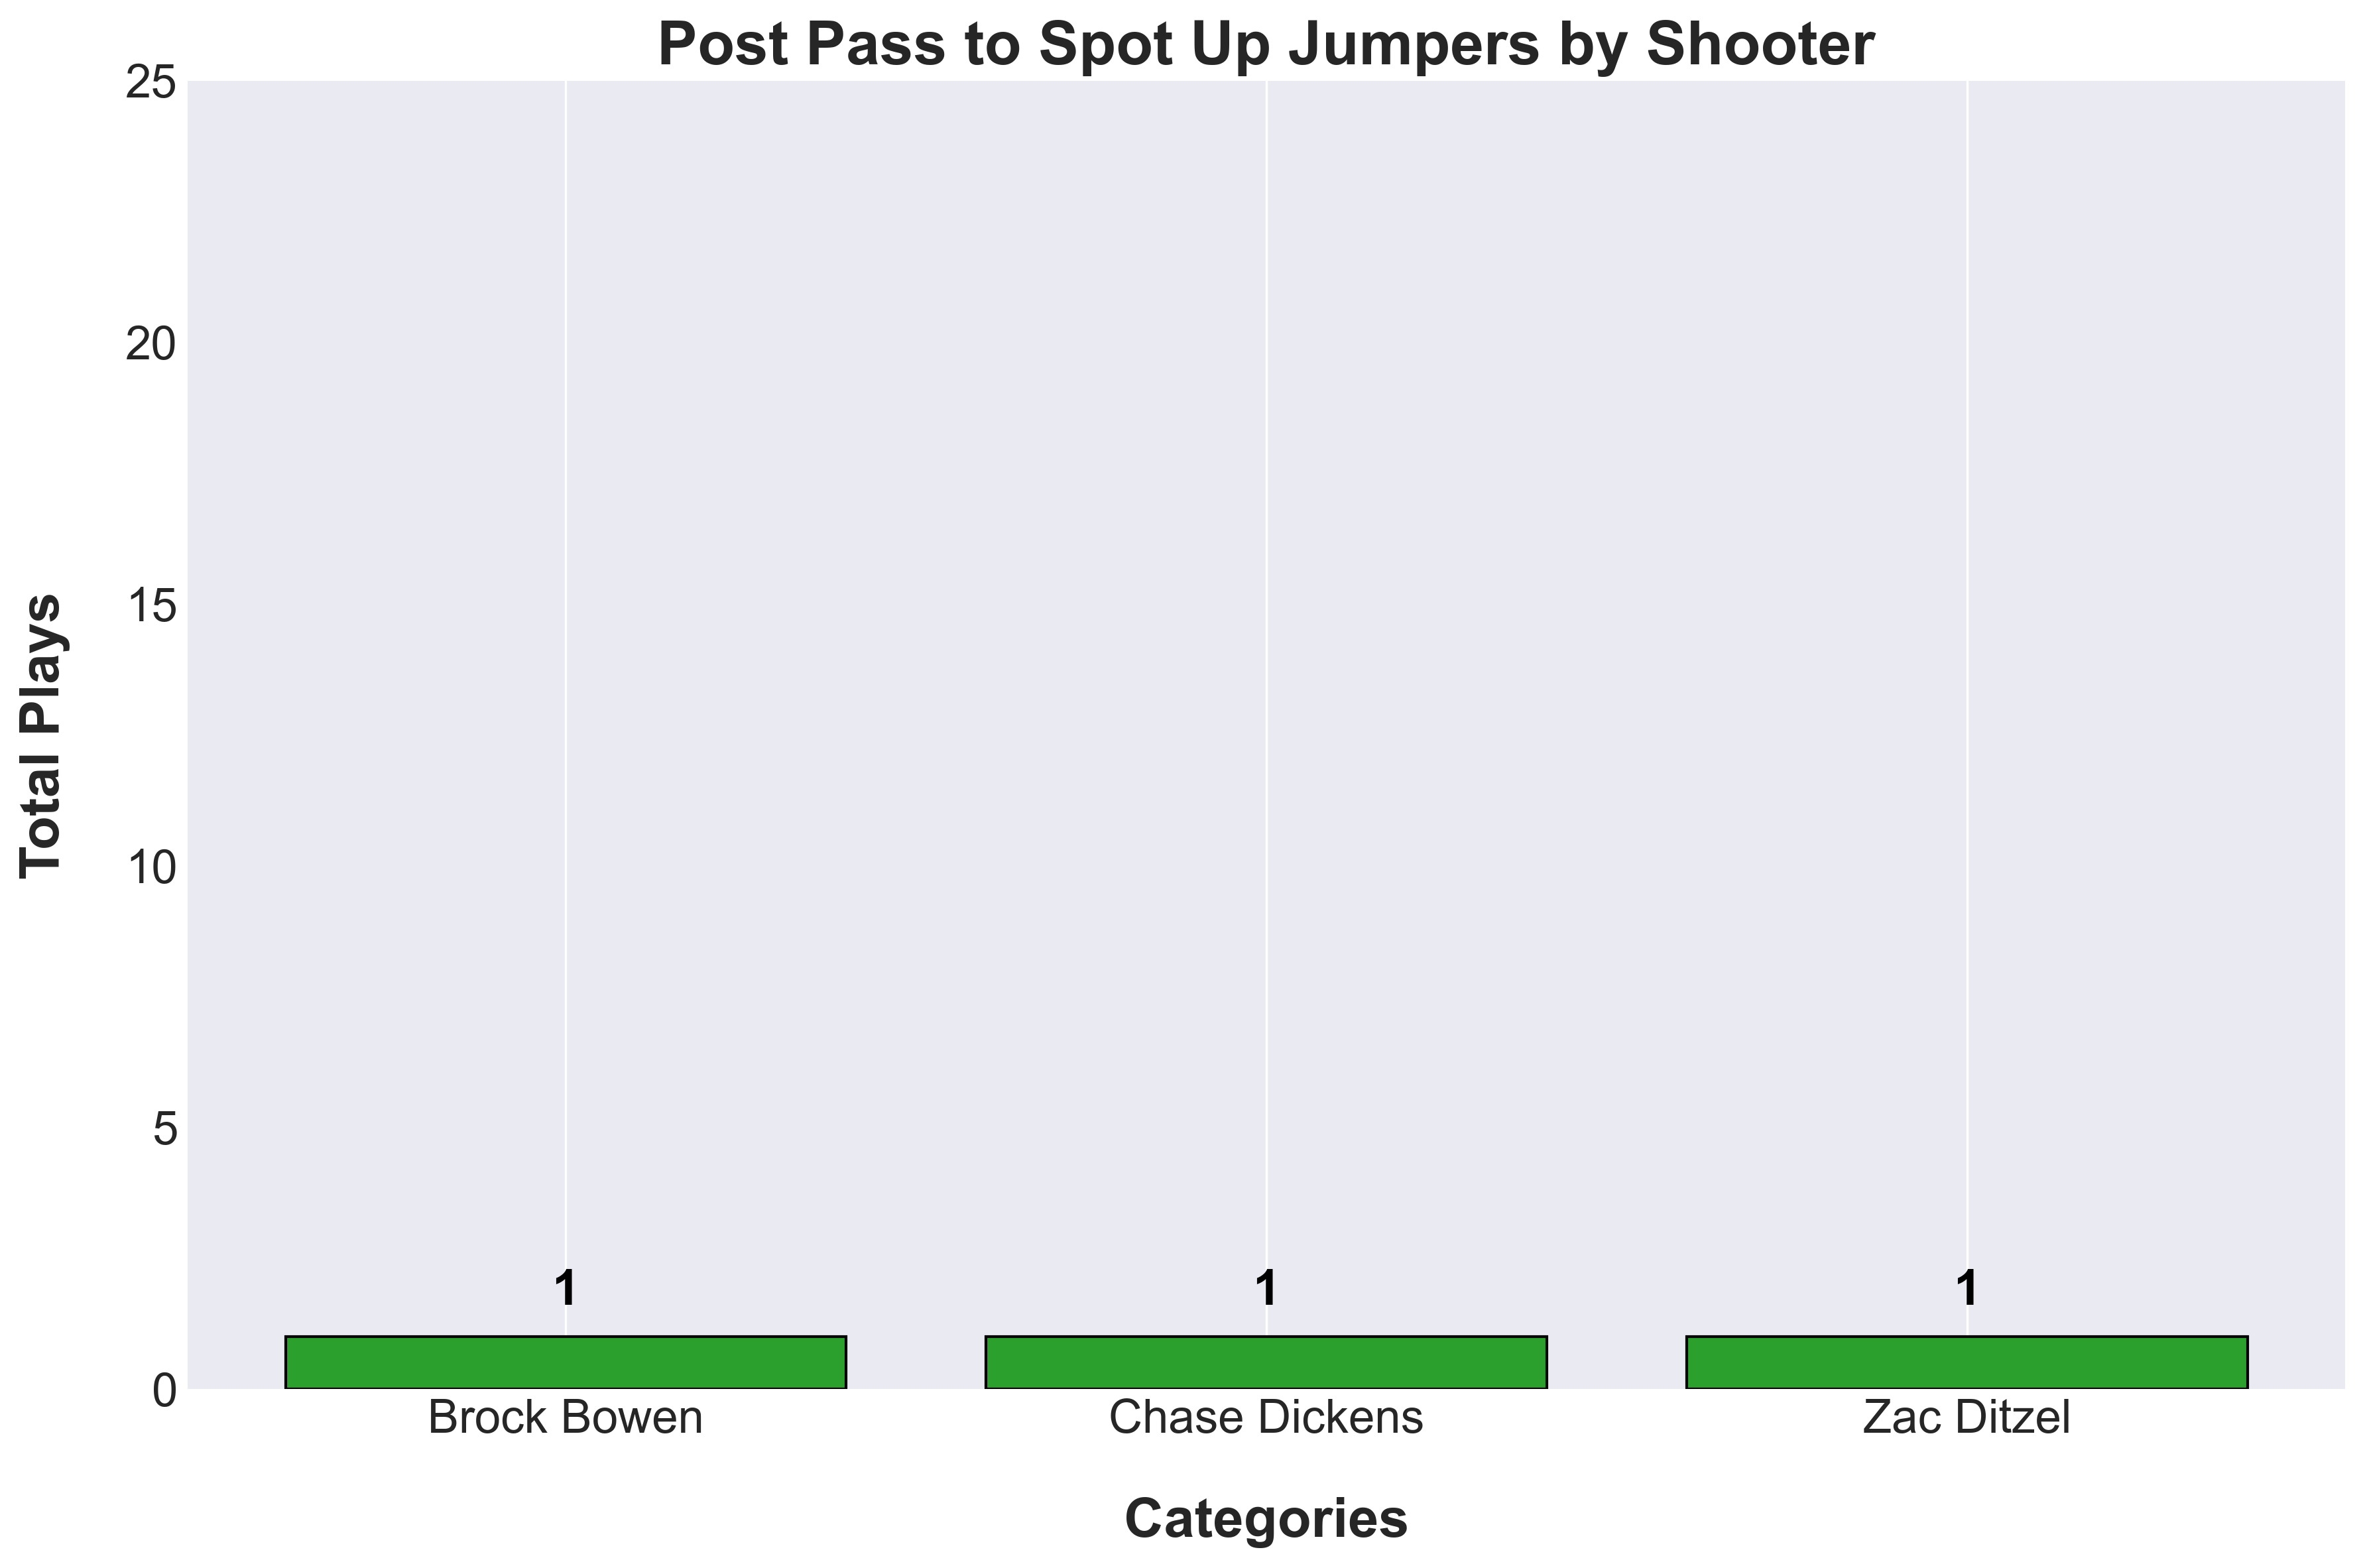
\includegraphics[width=\textwidth, height=.14\textheight]{images/Post_PassShotsPlayer_Freq.png} % Adjust the width of the image to fit
    \end{minipage}
\end{table}

\vspace{-1em} % Add vertical space before the line (optional)
\hrule height 1pt width 1\textwidth % Adjust height and width
\vspace{1em} % Add vertical space after the line (optional)





% ----------------------
% Rollman Visuals and Insights Section
% ----------------------
\subsection{Rollman}

\vspace{1em} % Add vertical space after the line (optional)
\hrule height 1pt width 1\textwidth % Adjust height and width
\vspace{1em} % Add vertical space after the line (optional)

\subsubsection{Rollman General Scorer Stats}
% All Rollman Statistics Table w/ room for insights
\begin{table}[H]
    \centering
    \begin{minipage}[t]{0.6\textwidth} % Left side (table) takes 85% of the width
        %\flushright
        \centering % Centering the title and the table
        \text{Total Rollman Shot Statistics} % Title above the table in bold
        \vskip .25em % Adds vertical space between title and table
        \scalebox{.85}{ % Scale the entire table down by half
            \scriptsize % Reduce the font size
            \begin{tabular}{
            >{\centering\arraybackslash}p{.75cm} 
            >{\centering\arraybackslash}p{.5cm} 
            >{\centering\arraybackslash}p{.5cm} 
            >{\centering\arraybackslash}p{.5cm}
            >{\centering\arraybackslash}p{.5cm} 
            >{\centering\arraybackslash}p{.5cm} 
            >{\centering\arraybackslash}p{.5cm} 
            >{\centering\arraybackslash}p{.5cm}
            >{\centering\arraybackslash}p{.5cm} 
            >{\centering\arraybackslash}p{.5cm}
            >{\centering\arraybackslash}p{.5cm} 
            >{\centering\arraybackslash}p{.5cm}}% Adjust column widths
            \toprule
            \textbf{Plays} &
            \textbf{3PA} &
            \textbf{3PM} &
            \textbf{3P\%} & 
            \textbf{2PA} & 
            \textbf{2PM} & 
            \textbf{2P\%} & 
            \textbf{MiA} & 
            \textbf{MiM} &
            \textbf{Mi\%} &
            \textbf{TO} &
            \textbf{Foul} \\
            \midrule
            
                
                    28 & 9 & 2 &
                    22.22 & 
                    14 & 8 &
                    57.14 &
                    0 & 0 &
                    - &
                    4 & 1 \\
                
            
                
            
                
            
                
            
                
            
                
            
                
            
                
            
                
            
                
            
                
            
                
            
                
            
                
            
                
            
                
            
            \bottomrule
            \end{tabular}
        }
    \end{minipage}
\end{table}

\vspace{0em} % Add vertical space before the line (optional)
%\hrule height 1pt width 1\textwidth % Adjust height and width
\vspace{-1em} % Add vertical space after the line (optional)

% Rollman Stats for Slip vs Pop vs Roll 
\begin{table}[H]
    \raisebox{3em}{ % Adjust this value to shift the tables vertically
    \begin{minipage}[t]{0.6\textwidth} % Left side (table) takes 85% of the width
        \flushleft
        \centering % Centering the title and the table
        \text{Rollman Play Type Statistics} % Title above the table in bold
        \vskip .25em % Adds vertical space between title and table
        \scalebox{.6}{ % Scale the entire table down by half
            \renewcommand{\arraystretch}{1.4} % Adjust the number to increase or decrease row spacing
            \begin{tabular}{
            >{\centering\arraybackslash}p{1.75cm} 
            >{\centering\arraybackslash}p{.75cm} 
            >{\centering\arraybackslash}p{.75cm} 
            >{\centering\arraybackslash}p{.75cm} 
            >{\centering\arraybackslash}p{.75cm}
            >{\centering\arraybackslash}p{.75cm} 
            >{\centering\arraybackslash}p{.75cm} 
            >{\centering\arraybackslash}p{.75cm} 
            >{\centering\arraybackslash}p{.75cm}
            >{\centering\arraybackslash}p{.75cm} 
            >{\centering\arraybackslash}p{.75cm}
            >{\centering\arraybackslash}p{.75cm} 
            >{\centering\arraybackslash}p{.75cm}}% Adjust column widths
            \toprule
            {\scriptsize \textbf{PlayType}} &
            {\scriptsize \textbf{Plays}} &
            {\scriptsize \textbf{3PA}} &
            {\scriptsize \textbf{3PM}} &
            {\scriptsize \textbf{3P\%}} & 
            {\scriptsize \textbf{2PA}} & 
            {\scriptsize \textbf{2PM}} & 
            {\scriptsize \textbf{2P\%}} & 
            {\scriptsize \textbf{MiA}} & 
            {\scriptsize \textbf{MiM}} &
            {\scriptsize \textbf{Mi\%}} &
            {\scriptsize \textbf{TO}} &
            {\scriptsize \textbf{Foul}} \\
            \midrule
            
                
            
                
            
                
                    Slip & 1 & 1 & 0 &
                    0.0 & 
                    0 & 0 &
                    - &
                    0 & 0 &
                    - &
                    0 & 0 \\
                
            
                
                    Roll & 14 & 0 & 0 &
                    - & 
                    12 & 8 &
                    66.67 &
                    0 & 0 &
                    - &
                    2 & 0 \\
                
            
                
                    Pop & 13 & 8 & 2 &
                    25.0 & 
                    2 & 0 &
                    0.0 &
                    0 & 0 &
                    - &
                    2 & 1 \\
                
            
                
            
                
            
                
            
                
            
                
            
                
            
                
            
                
            
                
            
                
            
                
            


            \bottomrule
        \end{tabular}
        } % End of \scalebox
    \end{minipage}
    } % End of raisebox, closing the adjustment
    \hfill % This adds some flexible space between the table and the image
    \begin{minipage}[c]{0.35\textwidth} % Right side (image) takes 10% of the width
        \flushright
        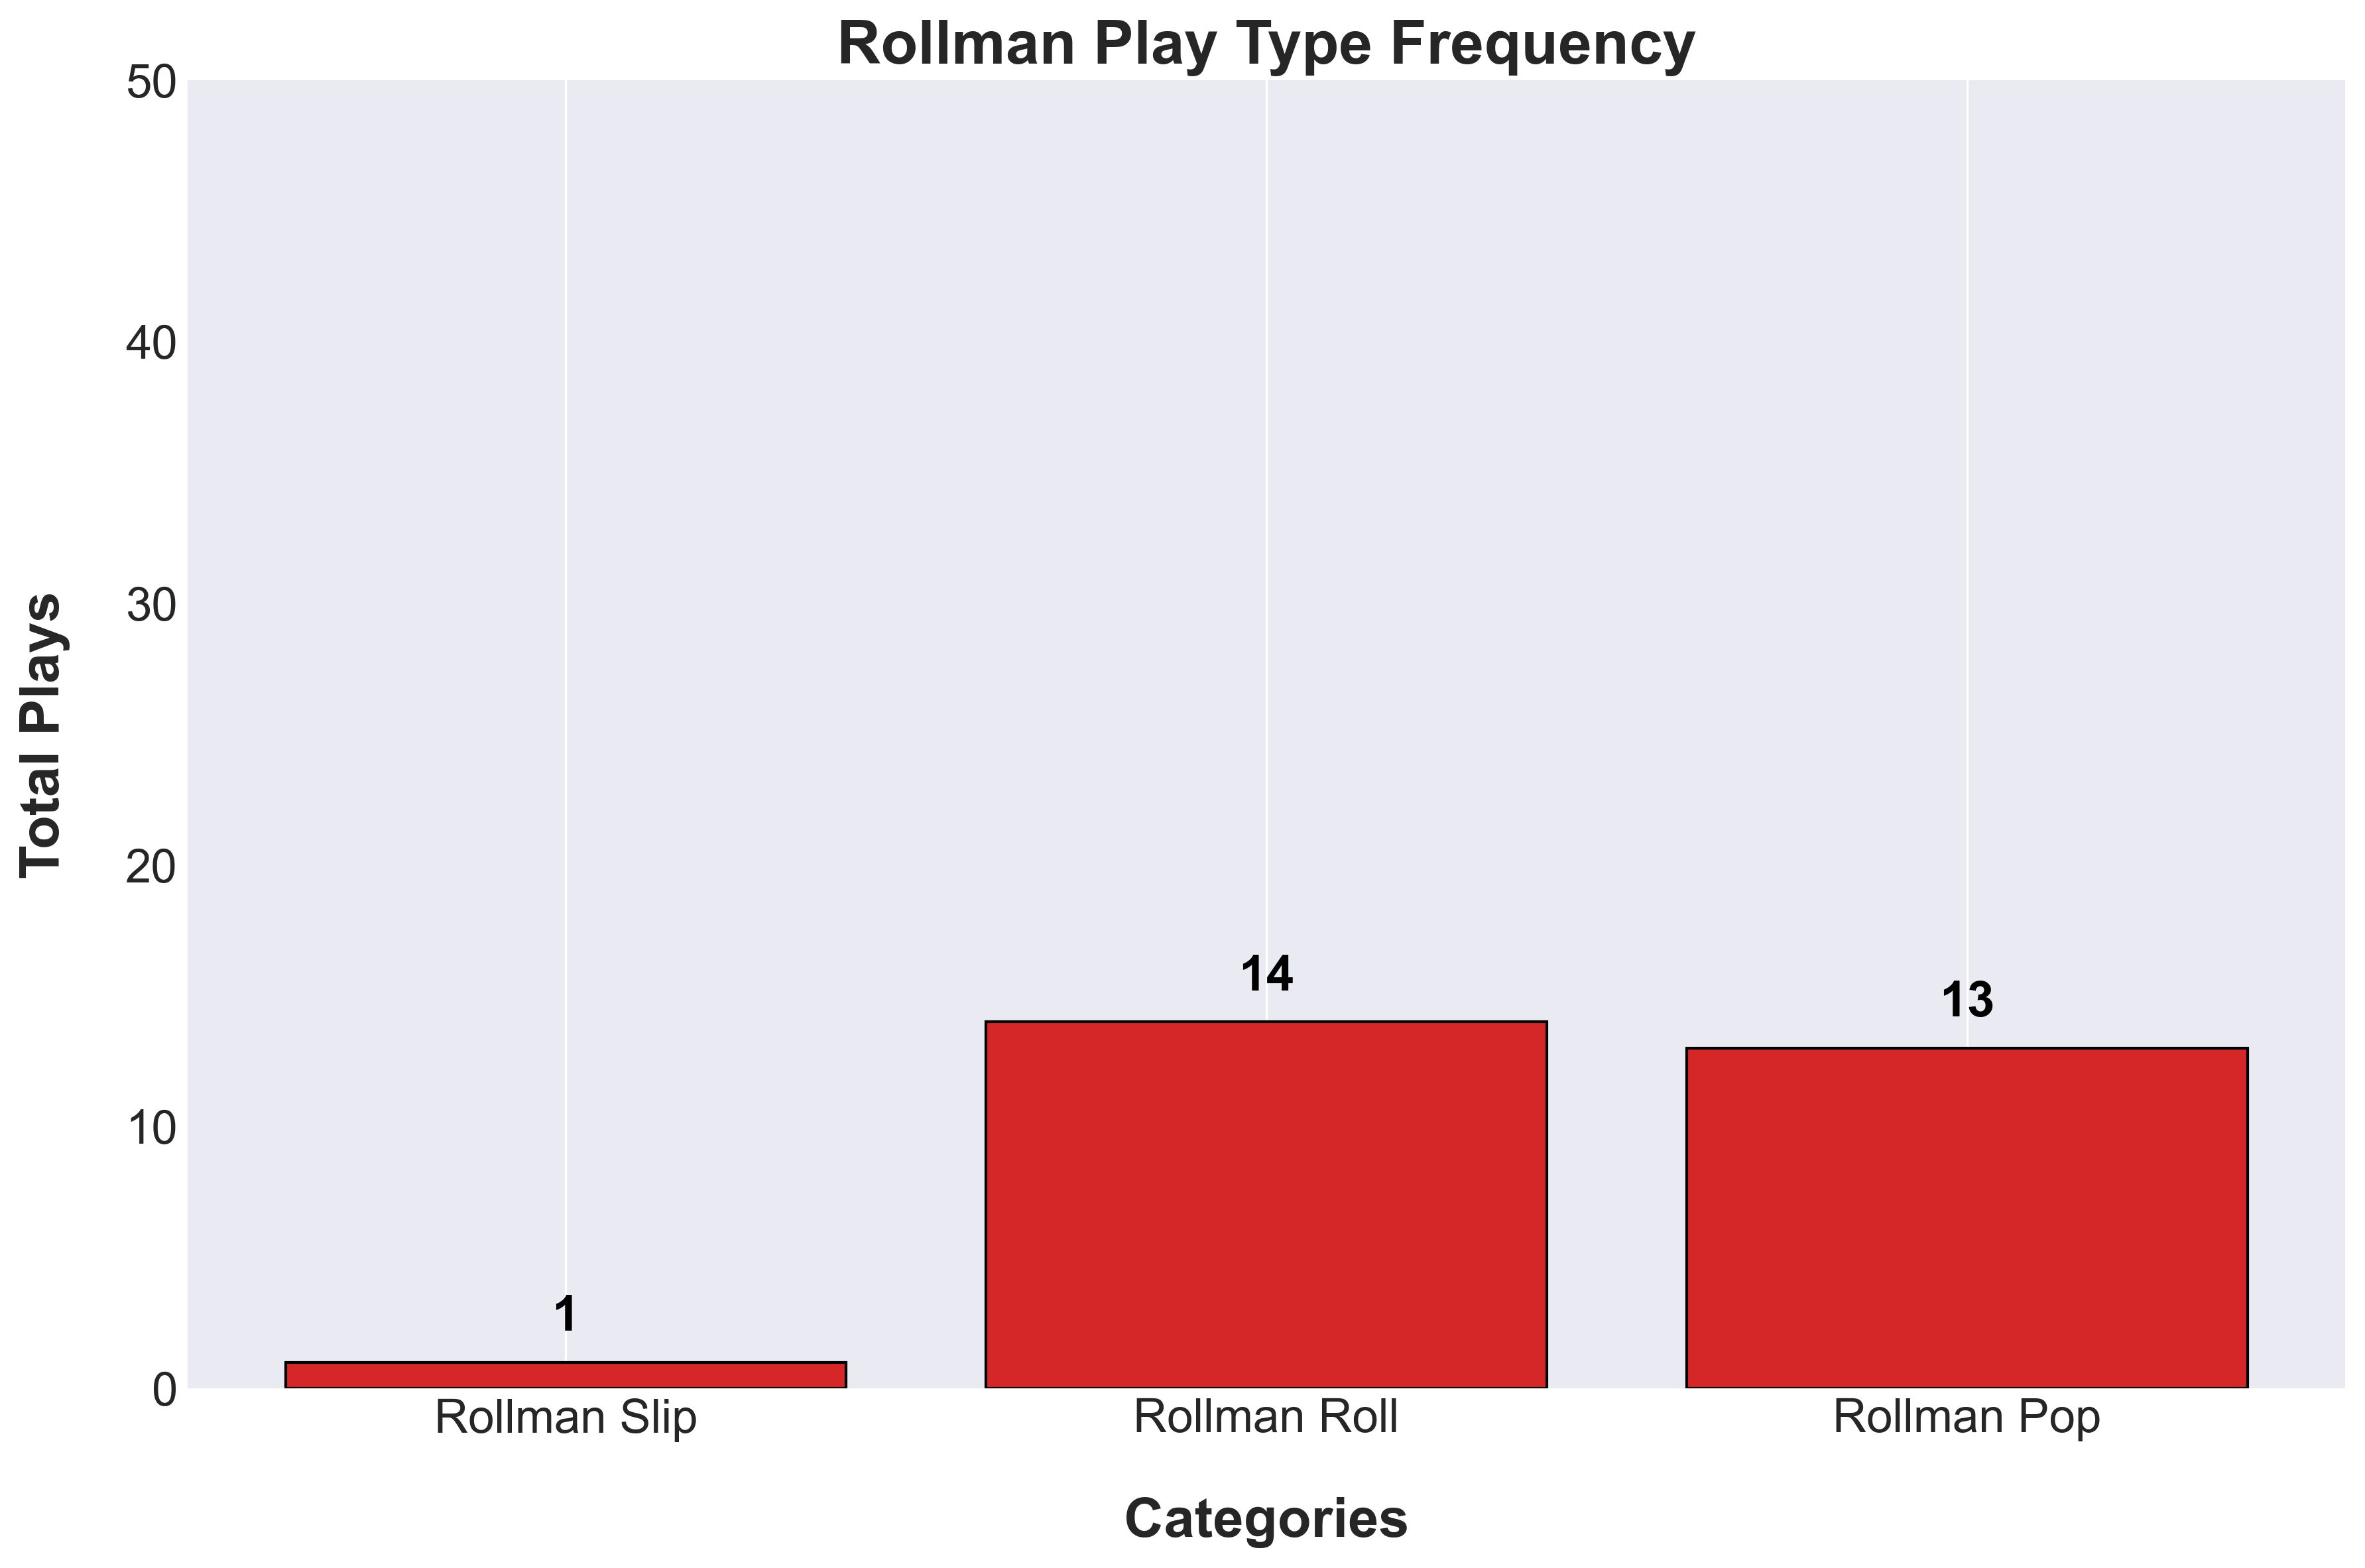
\includegraphics[width=\textwidth, height=.14\textheight]{images/Rollman_PlayType_Freq.png} % Adjust the width of the image to fit
    \end{minipage}
\end{table}

\vspace{-1em} % Add vertical space before the line (optional)
%\hrule height 1pt width 1\textwidth % Adjust height and width
\vspace{-1em} % Add vertical space after the line (optional)

% Rollman Slip Drive Direction
\begin{table}[H]
    \raisebox{3.5em}{ % Adjust this value to shift the tables vertically
    \begin{minipage}[t]{0.6\textwidth} % Left side (table) takes 85% of the width
        \flushleft
        \centering % Centering the title and the table
        \text{Rollman Slip to Drive Direction Statistics} % Title above the table in bold
        \vskip .25em % Adds vertical space between title and table
        \scalebox{.6}{ % Scale the entire table down by half
            \renewcommand{\arraystretch}{1.4} % Adjust the number to increase or decrease row spacing
            \begin{tabular}{
            >{\centering\arraybackslash}p{1.75cm} 
            >{\centering\arraybackslash}p{.75cm} 
            >{\centering\arraybackslash}p{.75cm} 
            >{\centering\arraybackslash}p{.75cm} 
            >{\centering\arraybackslash}p{.75cm}
            >{\centering\arraybackslash}p{.75cm} 
            >{\centering\arraybackslash}p{.75cm} 
            >{\centering\arraybackslash}p{.75cm} 
            >{\centering\arraybackslash}p{.75cm}
            >{\centering\arraybackslash}p{.75cm} 
            >{\centering\arraybackslash}p{.75cm}
            >{\centering\arraybackslash}p{.75cm} 
            >{\centering\arraybackslash}p{.75cm}}% Adjust column widths
            \toprule
            {\scriptsize \textbf{PlayType}} &
            {\scriptsize \textbf{Plays}} &
            {\scriptsize \textbf{3PA}} &
            {\scriptsize \textbf{3PM}} &
            {\scriptsize \textbf{3P\%}} & 
            {\scriptsize \textbf{2PA}} & 
            {\scriptsize \textbf{2PM}} & 
            {\scriptsize \textbf{2P\%}} & 
            {\scriptsize \textbf{MiA}} & 
            {\scriptsize \textbf{MiM}} &
            {\scriptsize \textbf{Mi\%}} &
            {\scriptsize \textbf{TO}} &
            {\scriptsize \textbf{Foul}} \\
            \midrule
            
                
            
                
            
                
            
                
            
                
            
                
            
                
            
                
            
                
            
                
            
                
            
                
            
                
            
                
            
                
            
                
            


            \bottomrule
        \end{tabular}
        } % End of \scalebox
    \end{minipage}
    } % End of raisebox, closing the adjustment
    \hfill
    \begin{minipage}[c]{0.35\textwidth} % Right side (image) takes 10% of the width
        \flushright
        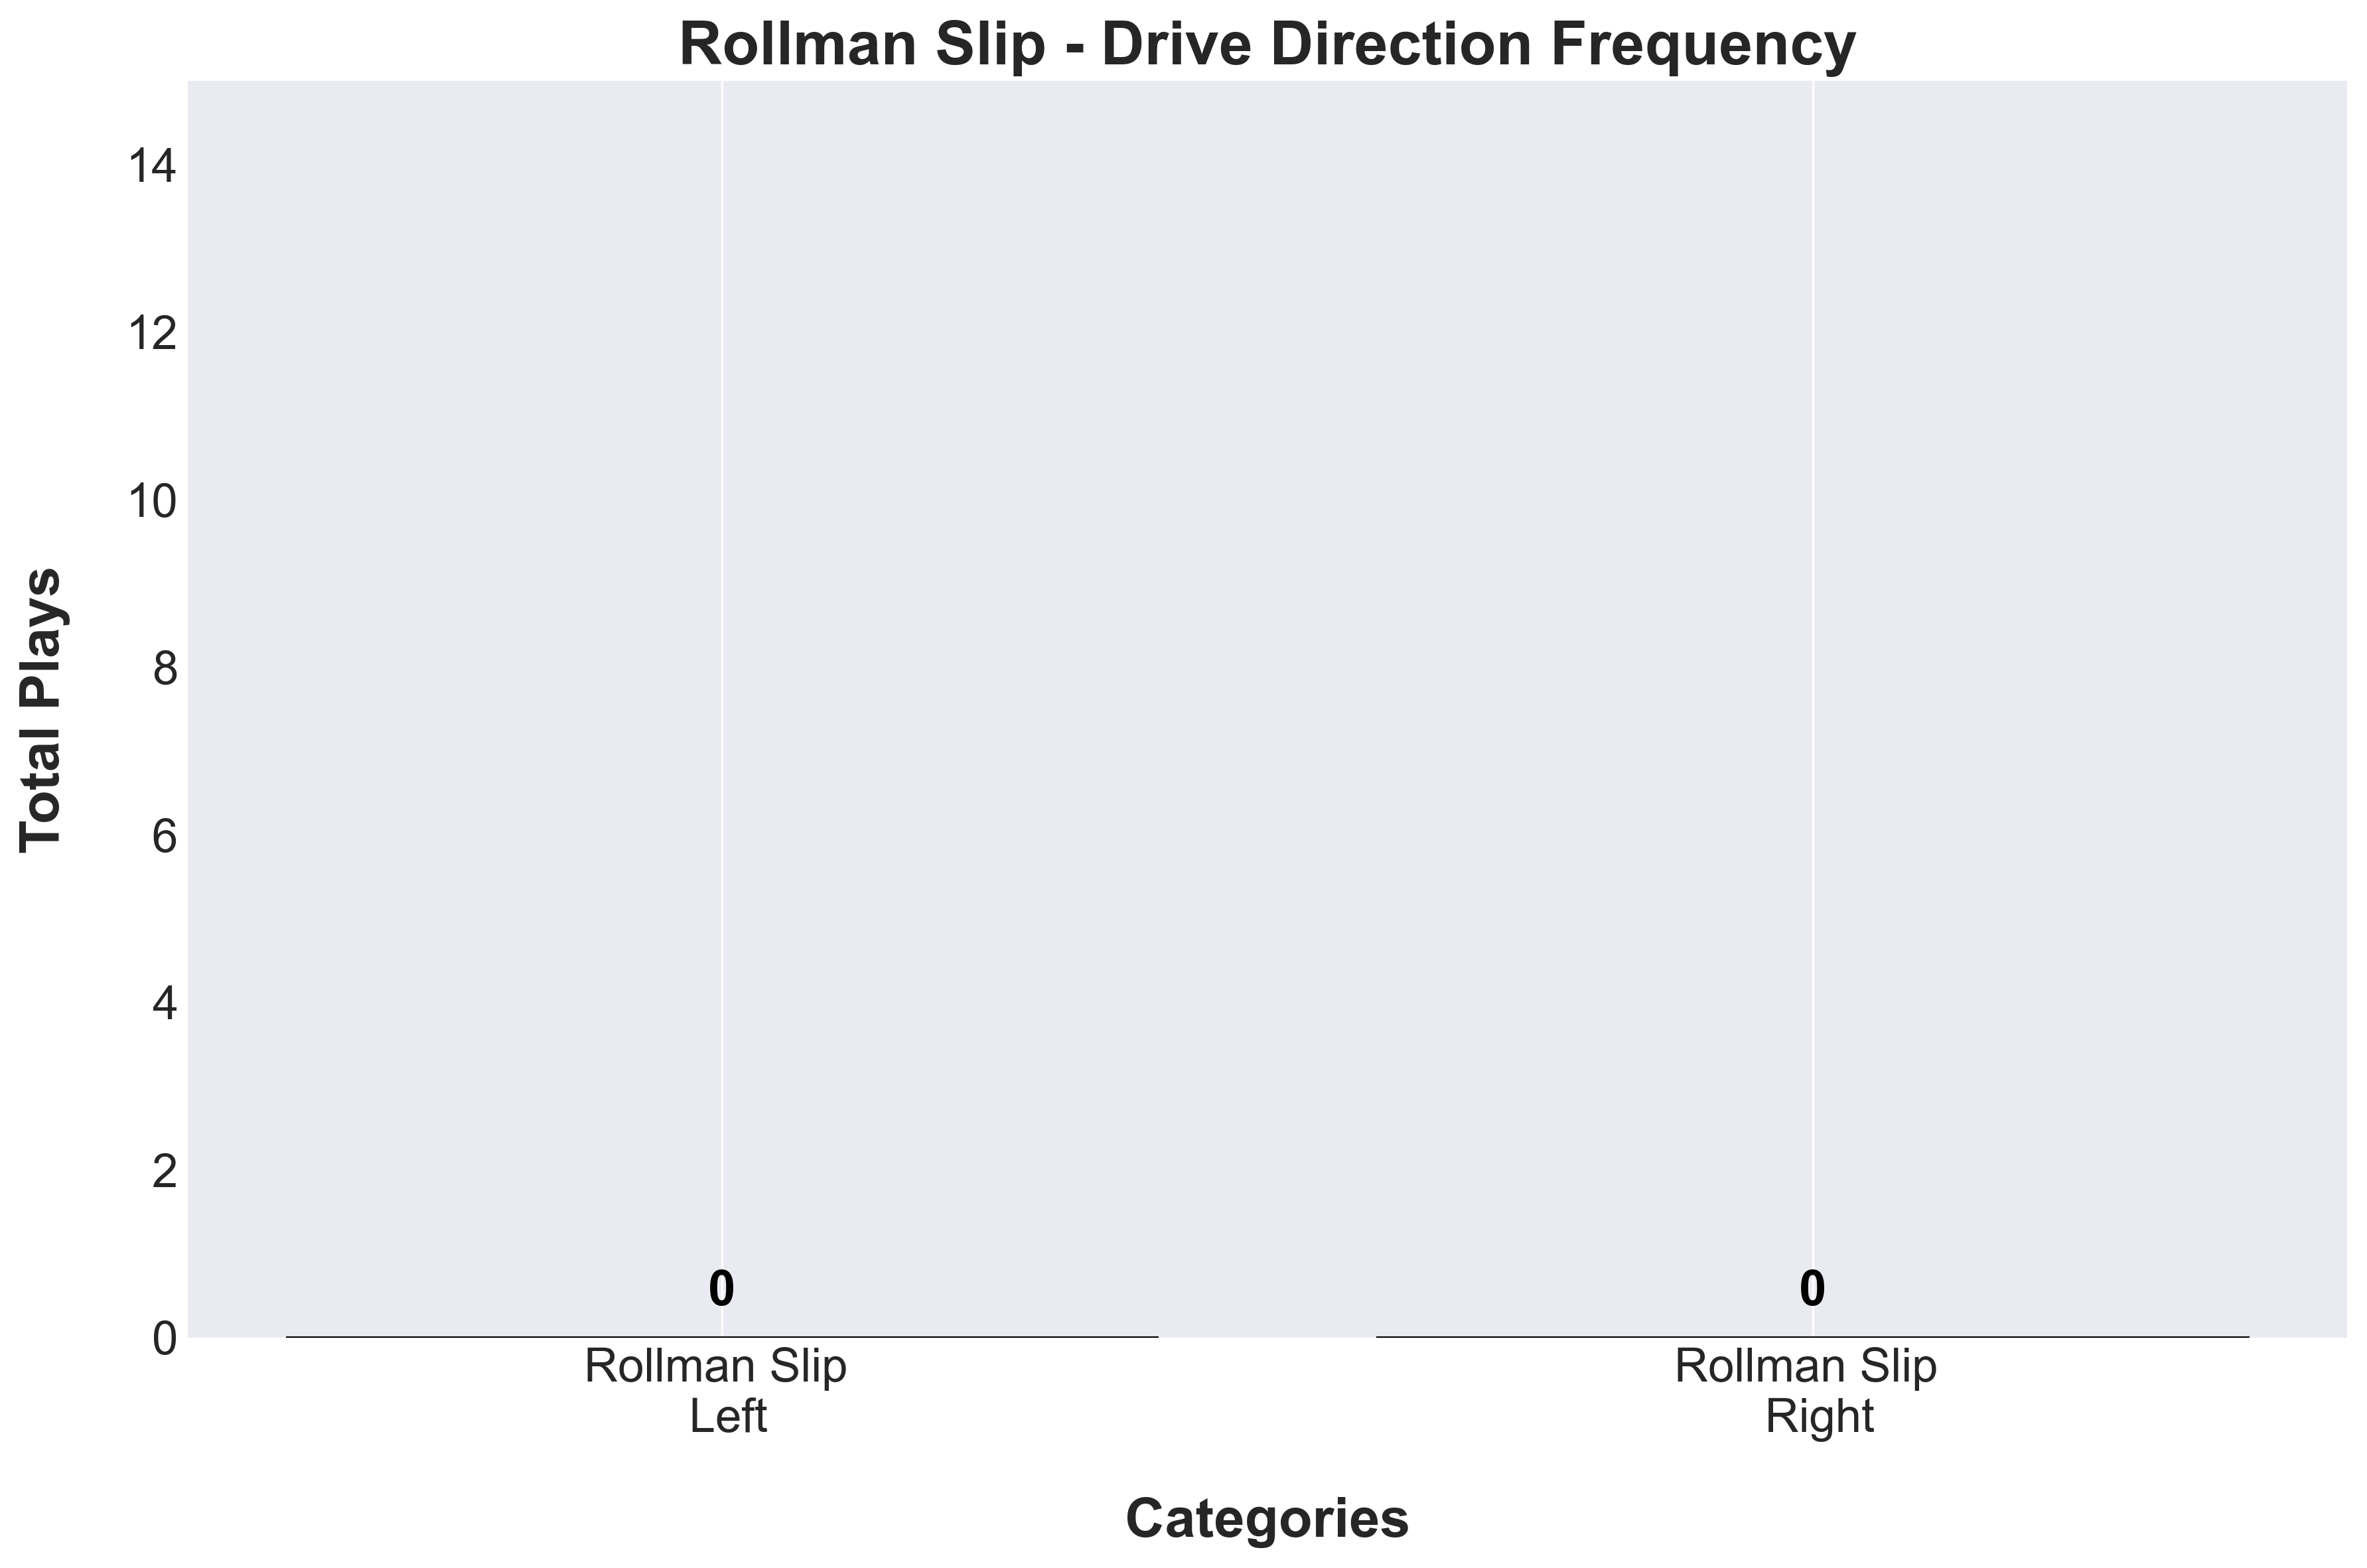
\includegraphics[width=\textwidth, height=.14\textheight]{images/Rollman_SlipDirection_Freq.png} % Adjust the width of the image to fit
    \end{minipage}
    
\end{table}

\vspace{-1em} % Add vertical space before the line (optional)
%\hrule height 1pt width 1\textwidth % Adjust height and width
\vspace{-1em} % Add vertical space after the line (optional)

% Rollman Pop Drive Direction
\begin{table}[H]
    \raisebox{3.5em}{ % Adjust this value to shift the tables vertically
    \begin{minipage}[t]{0.6\textwidth} % Left side (table) takes 85% of the width
        \flushleft
        \centering % Centering the title and the table
        \text{Rollman Pop to Drive Direction Statistics} % Title above the table in bold
        \vskip .25em % Adds vertical space between title and table
        \scalebox{.6}{ % Scale the entire table down by half
            \renewcommand{\arraystretch}{1.4} % Adjust the number to increase or decrease row spacing
            \begin{tabular}{
            >{\centering\arraybackslash}p{1.75cm} 
            >{\centering\arraybackslash}p{.75cm} 
            >{\centering\arraybackslash}p{.75cm} 
            >{\centering\arraybackslash}p{.75cm} 
            >{\centering\arraybackslash}p{.75cm}
            >{\centering\arraybackslash}p{.75cm} 
            >{\centering\arraybackslash}p{.75cm} 
            >{\centering\arraybackslash}p{.75cm} 
            >{\centering\arraybackslash}p{.75cm}
            >{\centering\arraybackslash}p{.75cm} 
            >{\centering\arraybackslash}p{.75cm}
            >{\centering\arraybackslash}p{.75cm} 
            >{\centering\arraybackslash}p{.75cm}}% Adjust column widths
            \toprule
            {\scriptsize \textbf{PlayType}} &
            {\scriptsize \textbf{Plays}} &
            {\scriptsize \textbf{3PA}} &
            {\scriptsize \textbf{3PM}} &
            {\scriptsize \textbf{3P\%}} & 
            {\scriptsize \textbf{2PA}} & 
            {\scriptsize \textbf{2PM}} & 
            {\scriptsize \textbf{2P\%}} & 
            {\scriptsize \textbf{MiA}} & 
            {\scriptsize \textbf{MiM}} &
            {\scriptsize \textbf{Mi\%}} &
            {\scriptsize \textbf{TO}} &
            {\scriptsize \textbf{Foul}} \\
            \midrule
            
                
            
                
            
                
            
                
            
                
            
                
            
                
            
                
            
                
            
                
            
                
                    Left & 2 & 0 & 0 &
                    - & 
                    0 & 0 &
                    - &
                    0 & 0 &
                    - &
                    1 & 1 \\
                
            
                
                    Right & 2 & 0 & 0 &
                    - & 
                    2 & 0 &
                    0.0 &
                    0 & 0 &
                    - &
                    0 & 0 \\
                
            
                
            
                
            
                
            
                
            


            \bottomrule
        \end{tabular}
        } % End of \scalebox
    \end{minipage}
    } % End of raisebox, closing the adjustment
    \hfill
    \begin{minipage}[c]{0.35\textwidth} % Right side (image) takes 10% of the width
        \flushright
        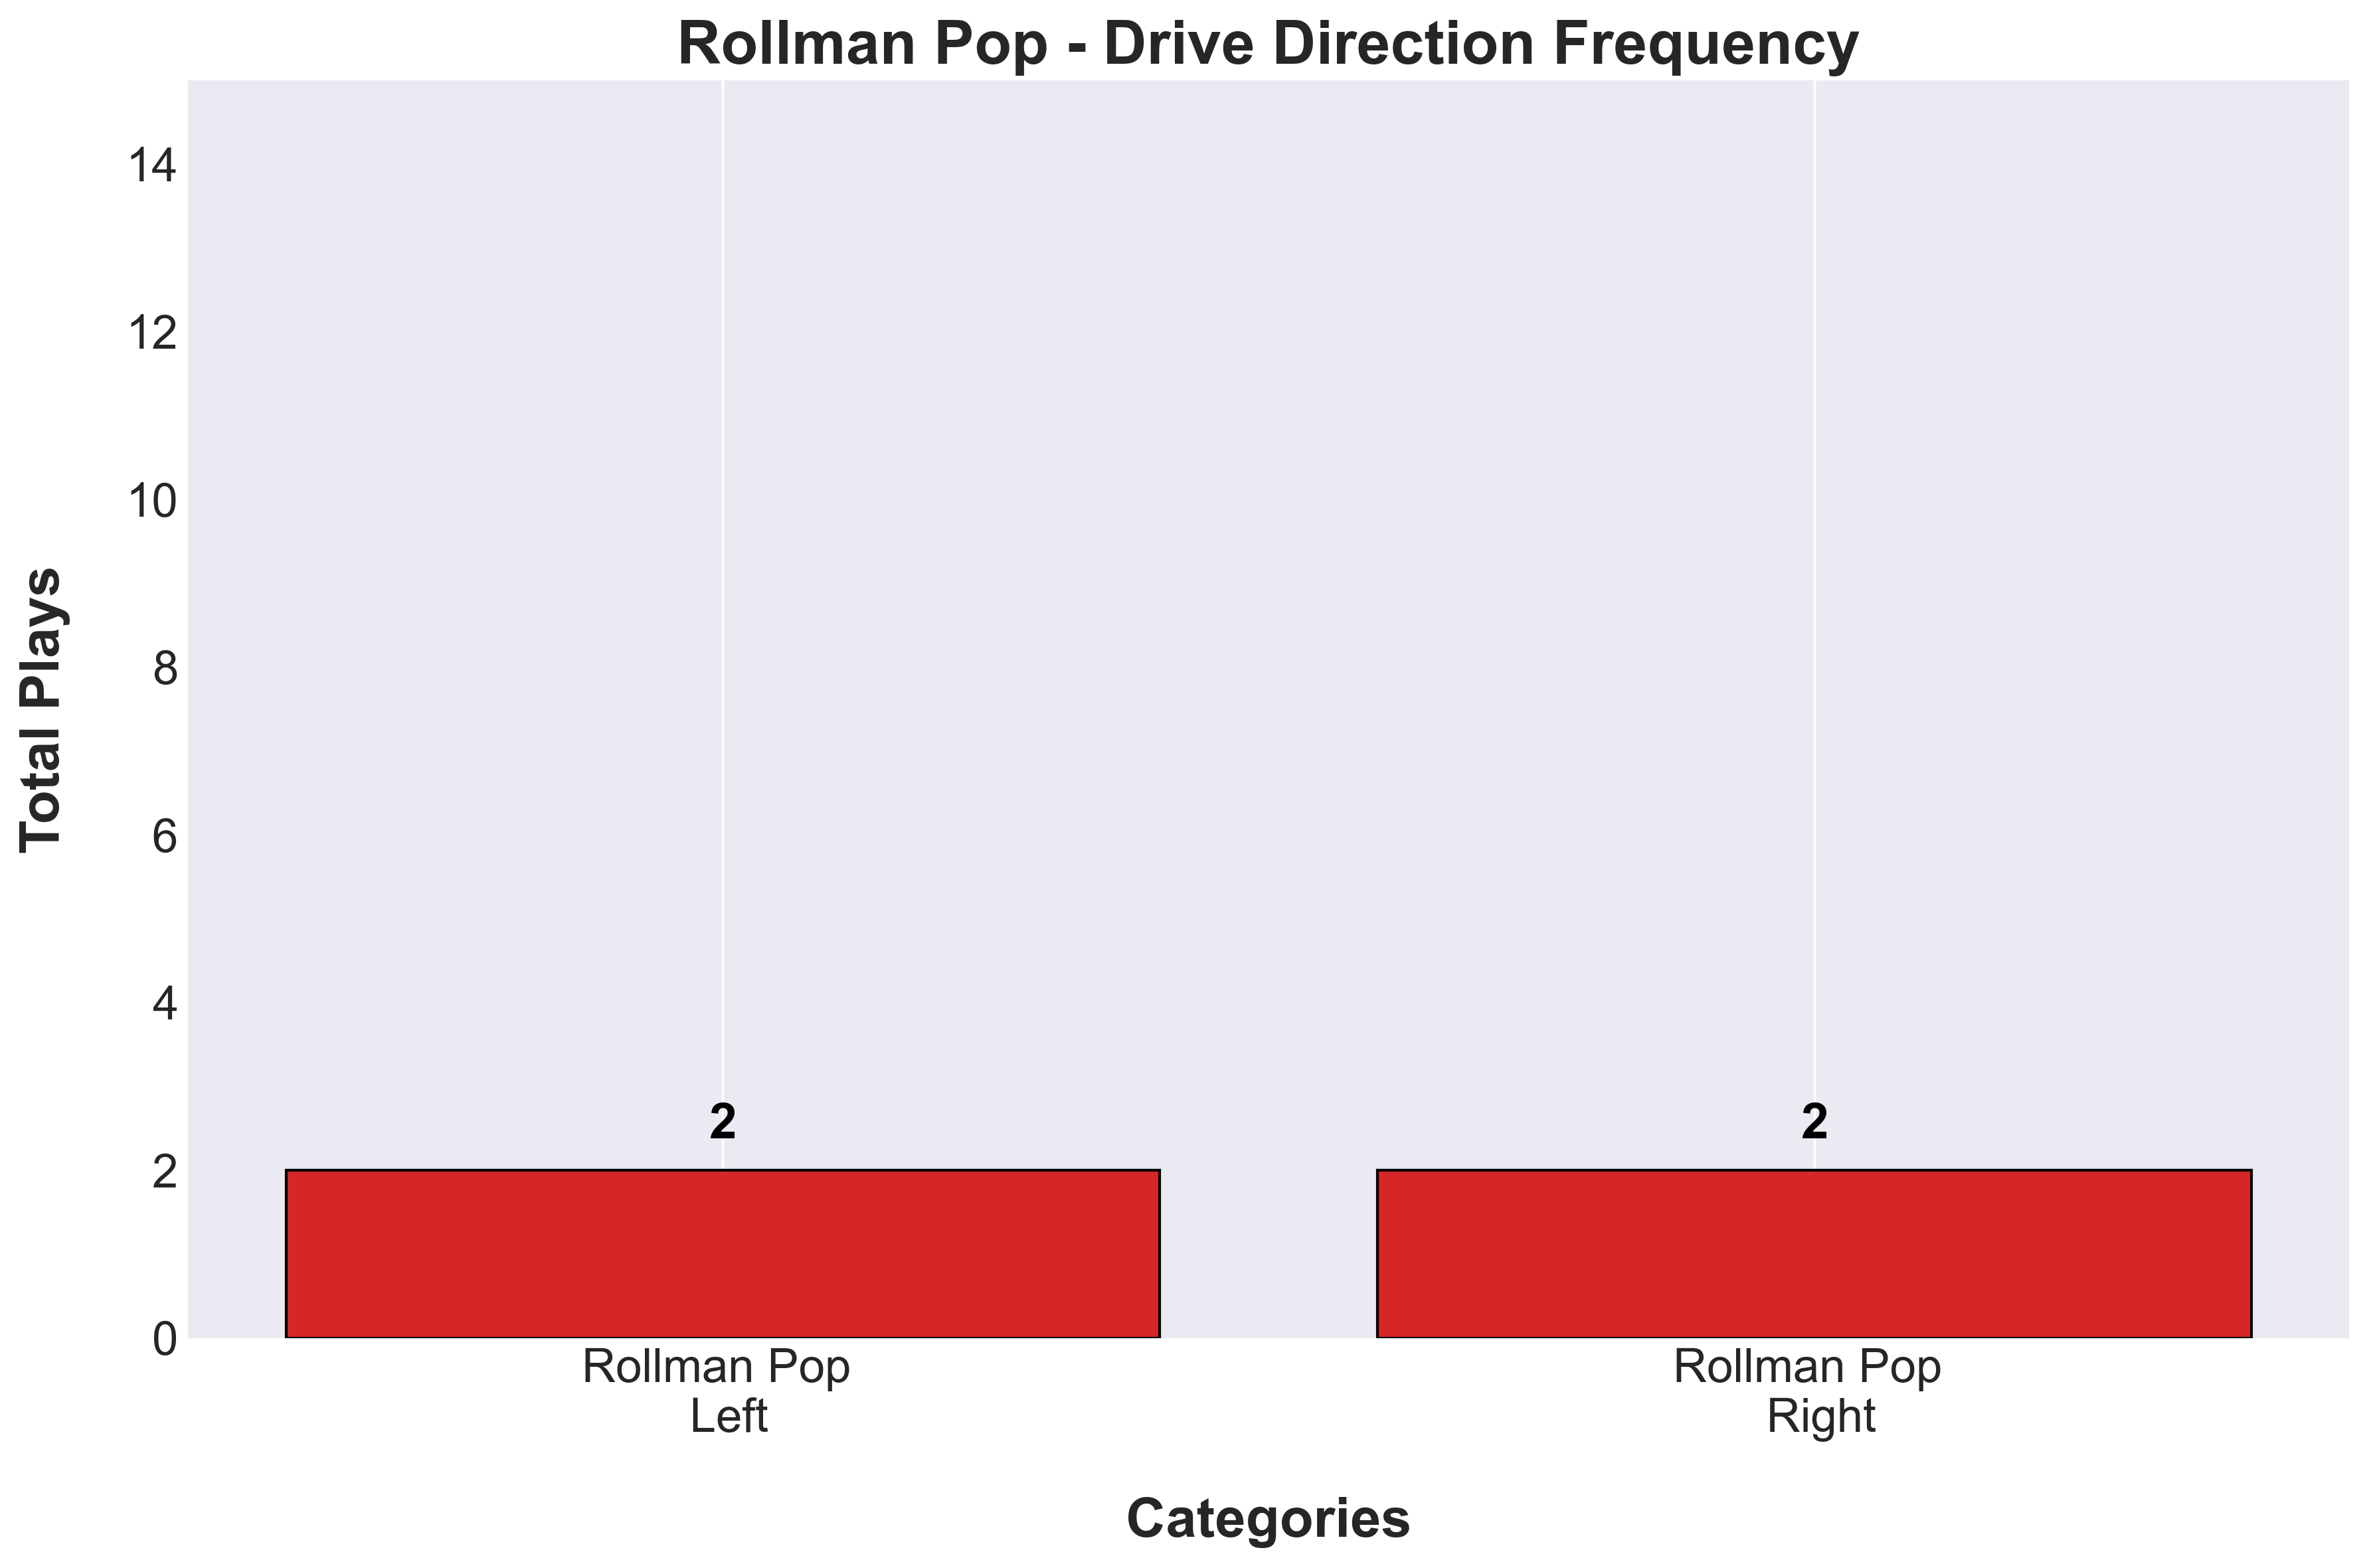
\includegraphics[width=\textwidth, height=.14\textheight]{images/Rollman_PopDirection_Freq.png} % Adjust the width of the image to fit
    \end{minipage}
    
\end{table}

\vspace{-1em} % Add vertical space before the line (optional)
\hrule height 1pt width 1\textwidth % Adjust height and width
\vspace{1em} % Add vertical space after the line (optional)

\subsubsection{Rollman by Passer Statistics}

\vspace{-1em} % Add vertical space before the line (optional)

% Rollman Slips Stats by Passer
\begin{table}[H]
    \raisebox{3em}{ % Adjust this value to shift the tables vertically
    \begin{minipage}[t]{0.6\textwidth} % Left side (table) takes 85% of the width
        \flushleft
        \centering % Centering the title and the table
        \text{Rollman Slip Stats by Passer} % Title above the table in bold
        \vskip .25em % Adds vertical space between title and table
        \scalebox{.55}{ % Scale the entire table down by half
            \renewcommand{\arraystretch}{1.4} % Adjust the number to increase or decrease row spacing
            \begin{tabular}{
            >{\centering\arraybackslash}p{3cm} 
            >{\centering\arraybackslash}p{.75cm} 
            >{\centering\arraybackslash}p{.75cm} 
            >{\centering\arraybackslash}p{.75cm} 
            >{\centering\arraybackslash}p{.75cm}
            >{\centering\arraybackslash}p{.75cm} 
            >{\centering\arraybackslash}p{.75cm} 
            >{\centering\arraybackslash}p{.75cm} 
            >{\centering\arraybackslash}p{.75cm}
            >{\centering\arraybackslash}p{.75cm} 
            >{\centering\arraybackslash}p{.75cm}
            >{\centering\arraybackslash}p{.75cm} 
            >{\centering\arraybackslash}p{.75cm}}% Adjust column widths
            \toprule
            {\scriptsize \textbf{Player}} &
            {\scriptsize \textbf{Plays}} &
            {\scriptsize \textbf{3PA}} &
            {\scriptsize \textbf{3PM}} &
            {\scriptsize \textbf{3P\%}} & 
            {\scriptsize \textbf{2PA}} & 
            {\scriptsize \textbf{2PM}} & 
            {\scriptsize \textbf{2P\%}} & 
            {\scriptsize \textbf{MiA}} & 
            {\scriptsize \textbf{MiM}} &
            {\scriptsize \textbf{Mi\%}} &
            {\scriptsize \textbf{TO}} &
            {\scriptsize \textbf{Foul}} \\
            \midrule
            
                
            
                
            
                
            
                
            
                
            
                
            
                
            
                
            
                
            
                
            
                
            
                
            
                
            
                
                    
                        Matt Caggiano & 
                        1 & 
                        1 & 
                        0 & 
                        0.0 & 
                        0 & 
                        0 & 
                        - & 
                        0 & 
                        0 & 
                        - & 
                        0 & 
                        0 \\
                    
                
            
                
            
                
            

            \bottomrule
        \end{tabular}
        } % End of \scalebox
    \end{minipage}
    } % End of raisebox, closing the adjustment
    \hfill % This adds some flexible space between the table and the image
    \begin{minipage}[c]{0.35\textwidth} % Right side (image) takes 10% of the width
        \flushright
        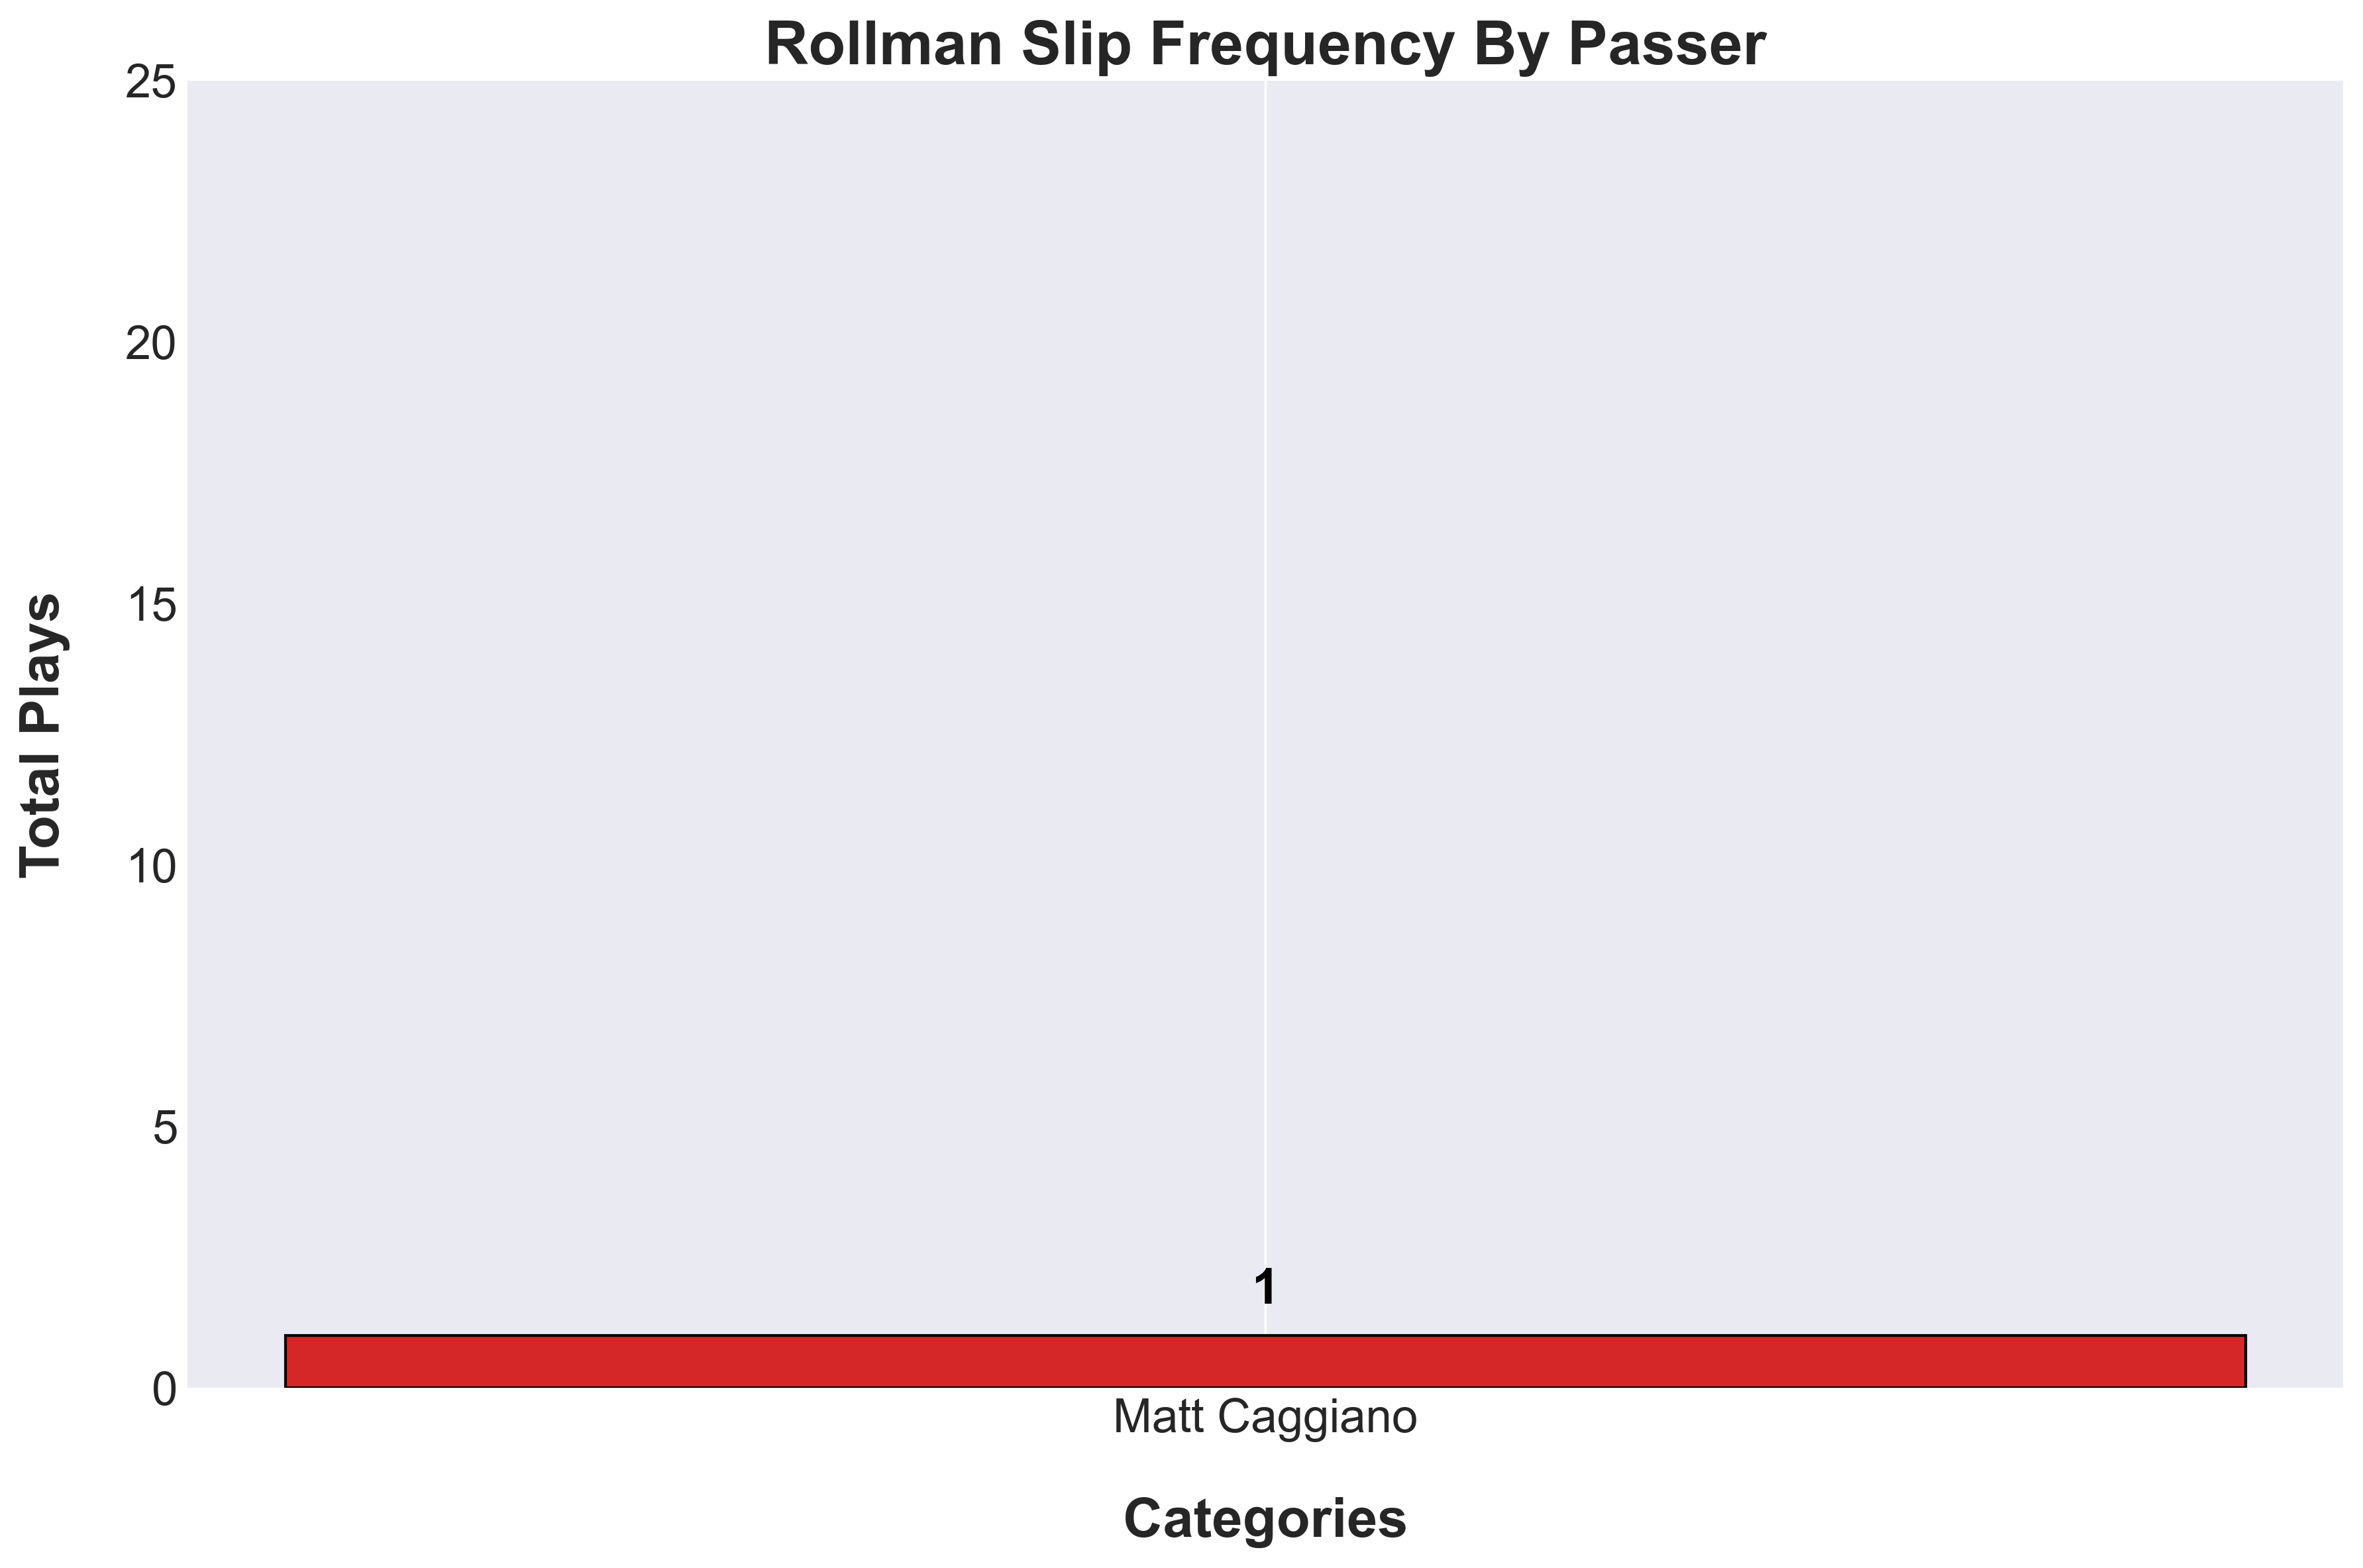
\includegraphics[width=\textwidth, height=.14\textheight]{images/Rollman_SlipPlayer_Freq.png} % Adjust the width of the image to fit
    \end{minipage}
\end{table}

\vspace{-1em} % Add vertical space before the line (optional)
\vspace{-1em} % Add vertical space after the line (optional)

% Rollman Pop Stats by Passer
\begin{table}[H]
    \raisebox{3em}{ % Adjust this value to shift the tables vertically
    \begin{minipage}[t]{0.6\textwidth} % Left side (table) takes 85% of the width
        \flushleft
        \centering % Centering the title and the table
        \text{Rollman Pop Stats by Passer} % Title above the table in bold
        \vskip .25em % Adds vertical space between title and table
        \scalebox{.55}{ % Scale the entire table down by half
            \renewcommand{\arraystretch}{1.4} % Adjust the number to increase or decrease row spacing
            \begin{tabular}{
            >{\centering\arraybackslash}p{3cm} 
            >{\centering\arraybackslash}p{.75cm} 
            >{\centering\arraybackslash}p{.75cm} 
            >{\centering\arraybackslash}p{.75cm} 
            >{\centering\arraybackslash}p{.75cm}
            >{\centering\arraybackslash}p{.75cm} 
            >{\centering\arraybackslash}p{.75cm} 
            >{\centering\arraybackslash}p{.75cm} 
            >{\centering\arraybackslash}p{.75cm}
            >{\centering\arraybackslash}p{.75cm} 
            >{\centering\arraybackslash}p{.75cm}
            >{\centering\arraybackslash}p{.75cm} 
            >{\centering\arraybackslash}p{.75cm}}% Adjust column widths
            \toprule
            {\scriptsize \textbf{Player}} &
            {\scriptsize \textbf{Plays}} &
            {\scriptsize \textbf{3PA}} &
            {\scriptsize \textbf{3PM}} &
            {\scriptsize \textbf{3P\%}} & 
            {\scriptsize \textbf{2PA}} & 
            {\scriptsize \textbf{2PM}} & 
            {\scriptsize \textbf{2P\%}} & 
            {\scriptsize \textbf{MiA}} & 
            {\scriptsize \textbf{MiM}} &
            {\scriptsize \textbf{Mi\%}} &
            {\scriptsize \textbf{TO}} &
            {\scriptsize \textbf{Foul}} \\
            \midrule
            
                
            
                
            
                
            
                
            
                
            
                
            
                
            
                
            
                
            
                
            
                
            
                
            
                
            
                
            
                
                    
                        Brock Bowen & 
                        3 & 
                        3 & 
                        1 & 
                        33.33 & 
                        0 & 
                        0 & 
                        - & 
                        0 & 
                        0 & 
                        - & 
                        0 & 
                        0 \\
                    
                        Brody Brown & 
                        1 & 
                        0 & 
                        0 & 
                        - & 
                        0 & 
                        0 & 
                        - & 
                        0 & 
                        0 & 
                        - & 
                        1 & 
                        0 \\
                    
                        Chase Dickens & 
                        1 & 
                        1 & 
                        0 & 
                        0.0 & 
                        0 & 
                        0 & 
                        - & 
                        0 & 
                        0 & 
                        - & 
                        0 & 
                        0 \\
                    
                        Keegan Ocorr & 
                        4 & 
                        1 & 
                        0 & 
                        0.0 & 
                        1 & 
                        0 & 
                        0.0 & 
                        0 & 
                        0 & 
                        - & 
                        1 & 
                        1 \\
                    
                        Luke Granto & 
                        1 & 
                        1 & 
                        0 & 
                        0.0 & 
                        0 & 
                        0 & 
                        - & 
                        0 & 
                        0 & 
                        - & 
                        0 & 
                        0 \\
                    
                        Matt Caggiano & 
                        3 & 
                        2 & 
                        1 & 
                        50.0 & 
                        1 & 
                        0 & 
                        0.0 & 
                        0 & 
                        0 & 
                        - & 
                        0 & 
                        0 \\
                    
                
            
                
            

            \bottomrule
        \end{tabular}
        } % End of \scalebox
    \end{minipage}
    } % End of raisebox, closing the adjustment
    \hfill % This adds some flexible space between the table and the image
    \begin{minipage}[c]{0.35\textwidth} % Right side (image) takes 10% of the width
        \flushright
        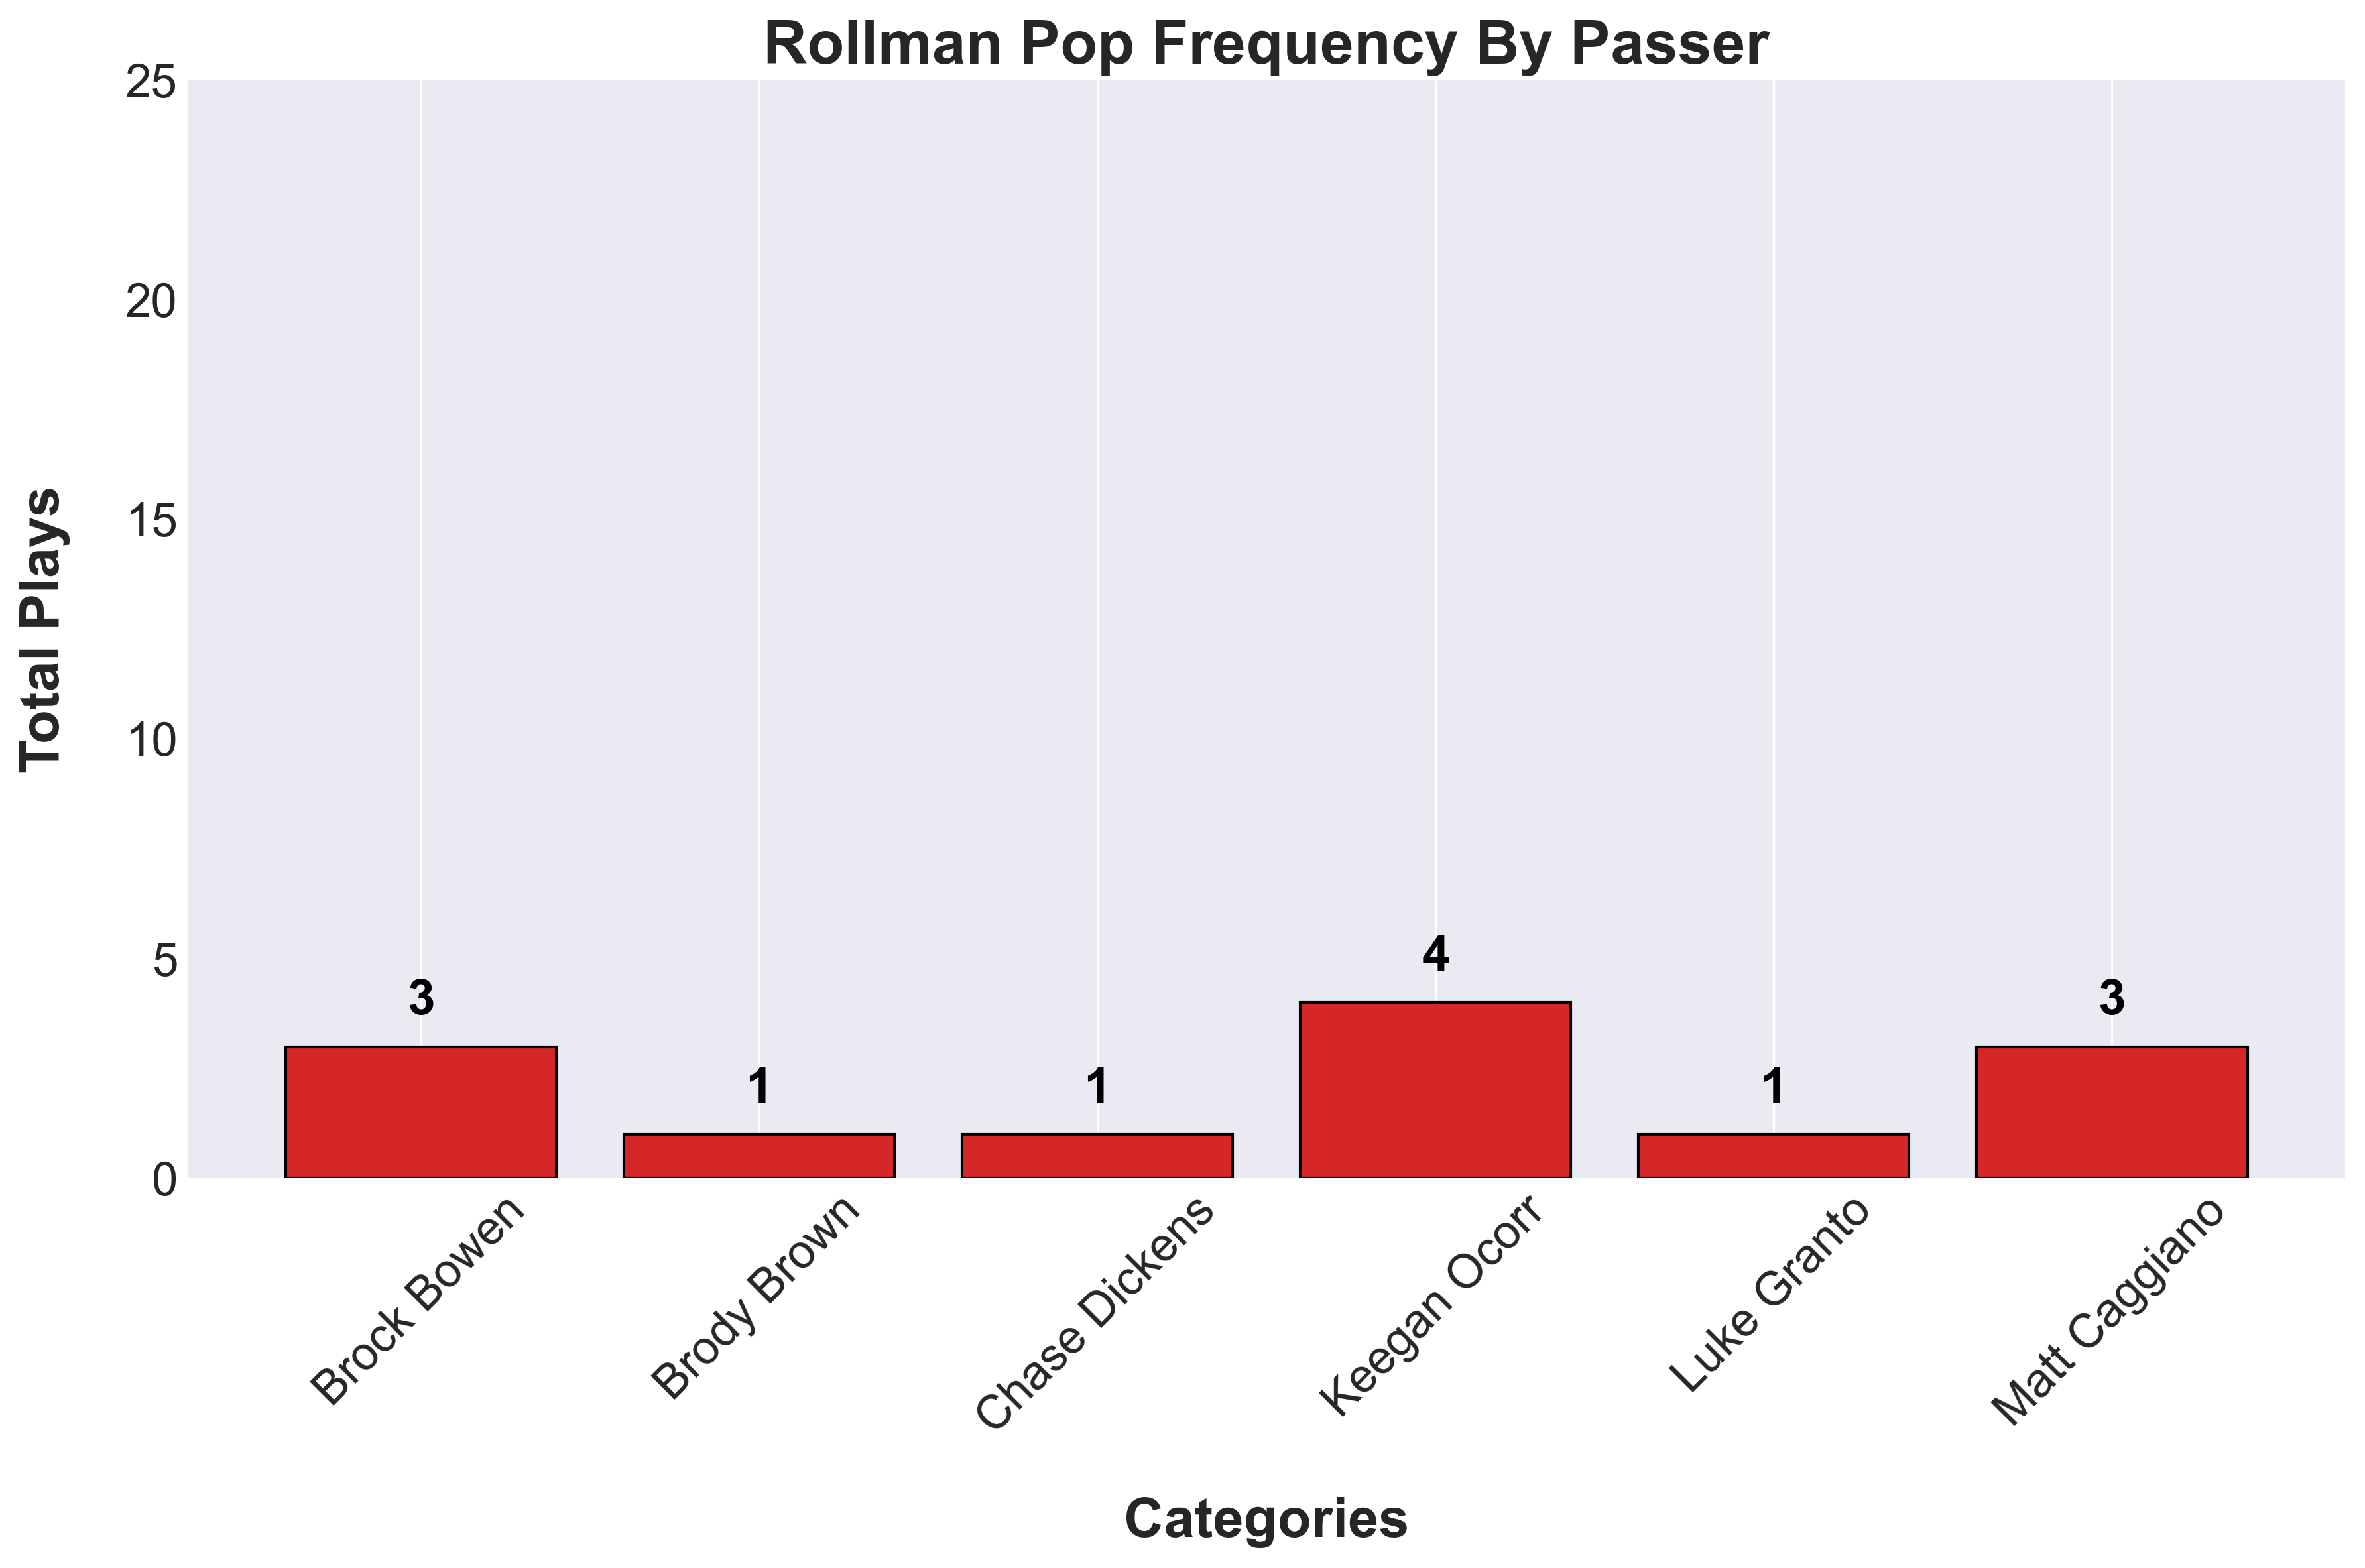
\includegraphics[width=\textwidth, height=.14\textheight]{images/Rollman_PopPlayer_Freq.png} % Adjust the width of the image to fit
    \end{minipage}
\end{table}

\vspace{-1em} % Add vertical space before the line (optional)
\vspace{-1em} % Add vertical space after the line (optional)

% Rollman Rolls Stats by Passer
\begin{table}[H]
    \raisebox{3em}{ % Adjust this value to shift the tables vertically
    \begin{minipage}[t]{0.6\textwidth} % Left side (table) takes 85% of the width
        \flushleft
        \centering % Centering the title and the table
        \text{Rollman Roll Stats by Passer} % Title above the table in bold
        \vskip .25em % Adds vertical space between title and table
        \scalebox{.55}{ % Scale the entire table down by half
            \renewcommand{\arraystretch}{1.4} % Adjust the number to increase or decrease row spacing
            \begin{tabular}{
            >{\centering\arraybackslash}p{3cm} 
            >{\centering\arraybackslash}p{.75cm} 
            >{\centering\arraybackslash}p{.75cm} 
            >{\centering\arraybackslash}p{.75cm} 
            >{\centering\arraybackslash}p{.75cm}
            >{\centering\arraybackslash}p{.75cm} 
            >{\centering\arraybackslash}p{.75cm} 
            >{\centering\arraybackslash}p{.75cm} 
            >{\centering\arraybackslash}p{.75cm}
            >{\centering\arraybackslash}p{.75cm} 
            >{\centering\arraybackslash}p{.75cm}
            >{\centering\arraybackslash}p{.75cm} 
            >{\centering\arraybackslash}p{.75cm}}% Adjust column widths
            \toprule
            {\scriptsize \textbf{Player}} &
            {\scriptsize \textbf{Plays}} &
            {\scriptsize \textbf{3PA}} &
            {\scriptsize \textbf{3PM}} &
            {\scriptsize \textbf{3P\%}} & 
            {\scriptsize \textbf{2PA}} & 
            {\scriptsize \textbf{2PM}} & 
            {\scriptsize \textbf{2P\%}} & 
            {\scriptsize \textbf{MiA}} & 
            {\scriptsize \textbf{MiM}} &
            {\scriptsize \textbf{Mi\%}} &
            {\scriptsize \textbf{TO}} &
            {\scriptsize \textbf{Foul}} \\
            \midrule
            
                
            
                
            
                
            
                
            
                
            
                
            
                
            
                
            
                
            
                
            
                
            
                
            
                
            
                
            
                
            
                
                    
                        Brandon Weiss & 
                        1 & 
                        0 & 
                        0 & 
                        - & 
                        1 & 
                        0 & 
                        0.0 & 
                        0 & 
                        0 & 
                        - & 
                        0 & 
                        0 \\
                    
                        Brock Bowen & 
                        3 & 
                        0 & 
                        0 & 
                        - & 
                        1 & 
                        1 & 
                        100.0 & 
                        0 & 
                        0 & 
                        - & 
                        2 & 
                        0 \\
                    
                        Chase Dickens & 
                        4 & 
                        0 & 
                        0 & 
                        - & 
                        4 & 
                        3 & 
                        75.0 & 
                        0 & 
                        0 & 
                        - & 
                        0 & 
                        0 \\
                    
                        Matt Caggiano & 
                        6 & 
                        0 & 
                        0 & 
                        - & 
                        6 & 
                        4 & 
                        66.67 & 
                        0 & 
                        0 & 
                        - & 
                        0 & 
                        0 \\
                    
                
            

            \bottomrule
        \end{tabular}
        } % End of \scalebox
    \end{minipage}
    } % End of raisebox, closing the adjustment
    \hfill % This adds some flexible space between the table and the image
    \begin{minipage}[c]{0.35\textwidth} % Right side (image) takes 10% of the width
        \flushright
        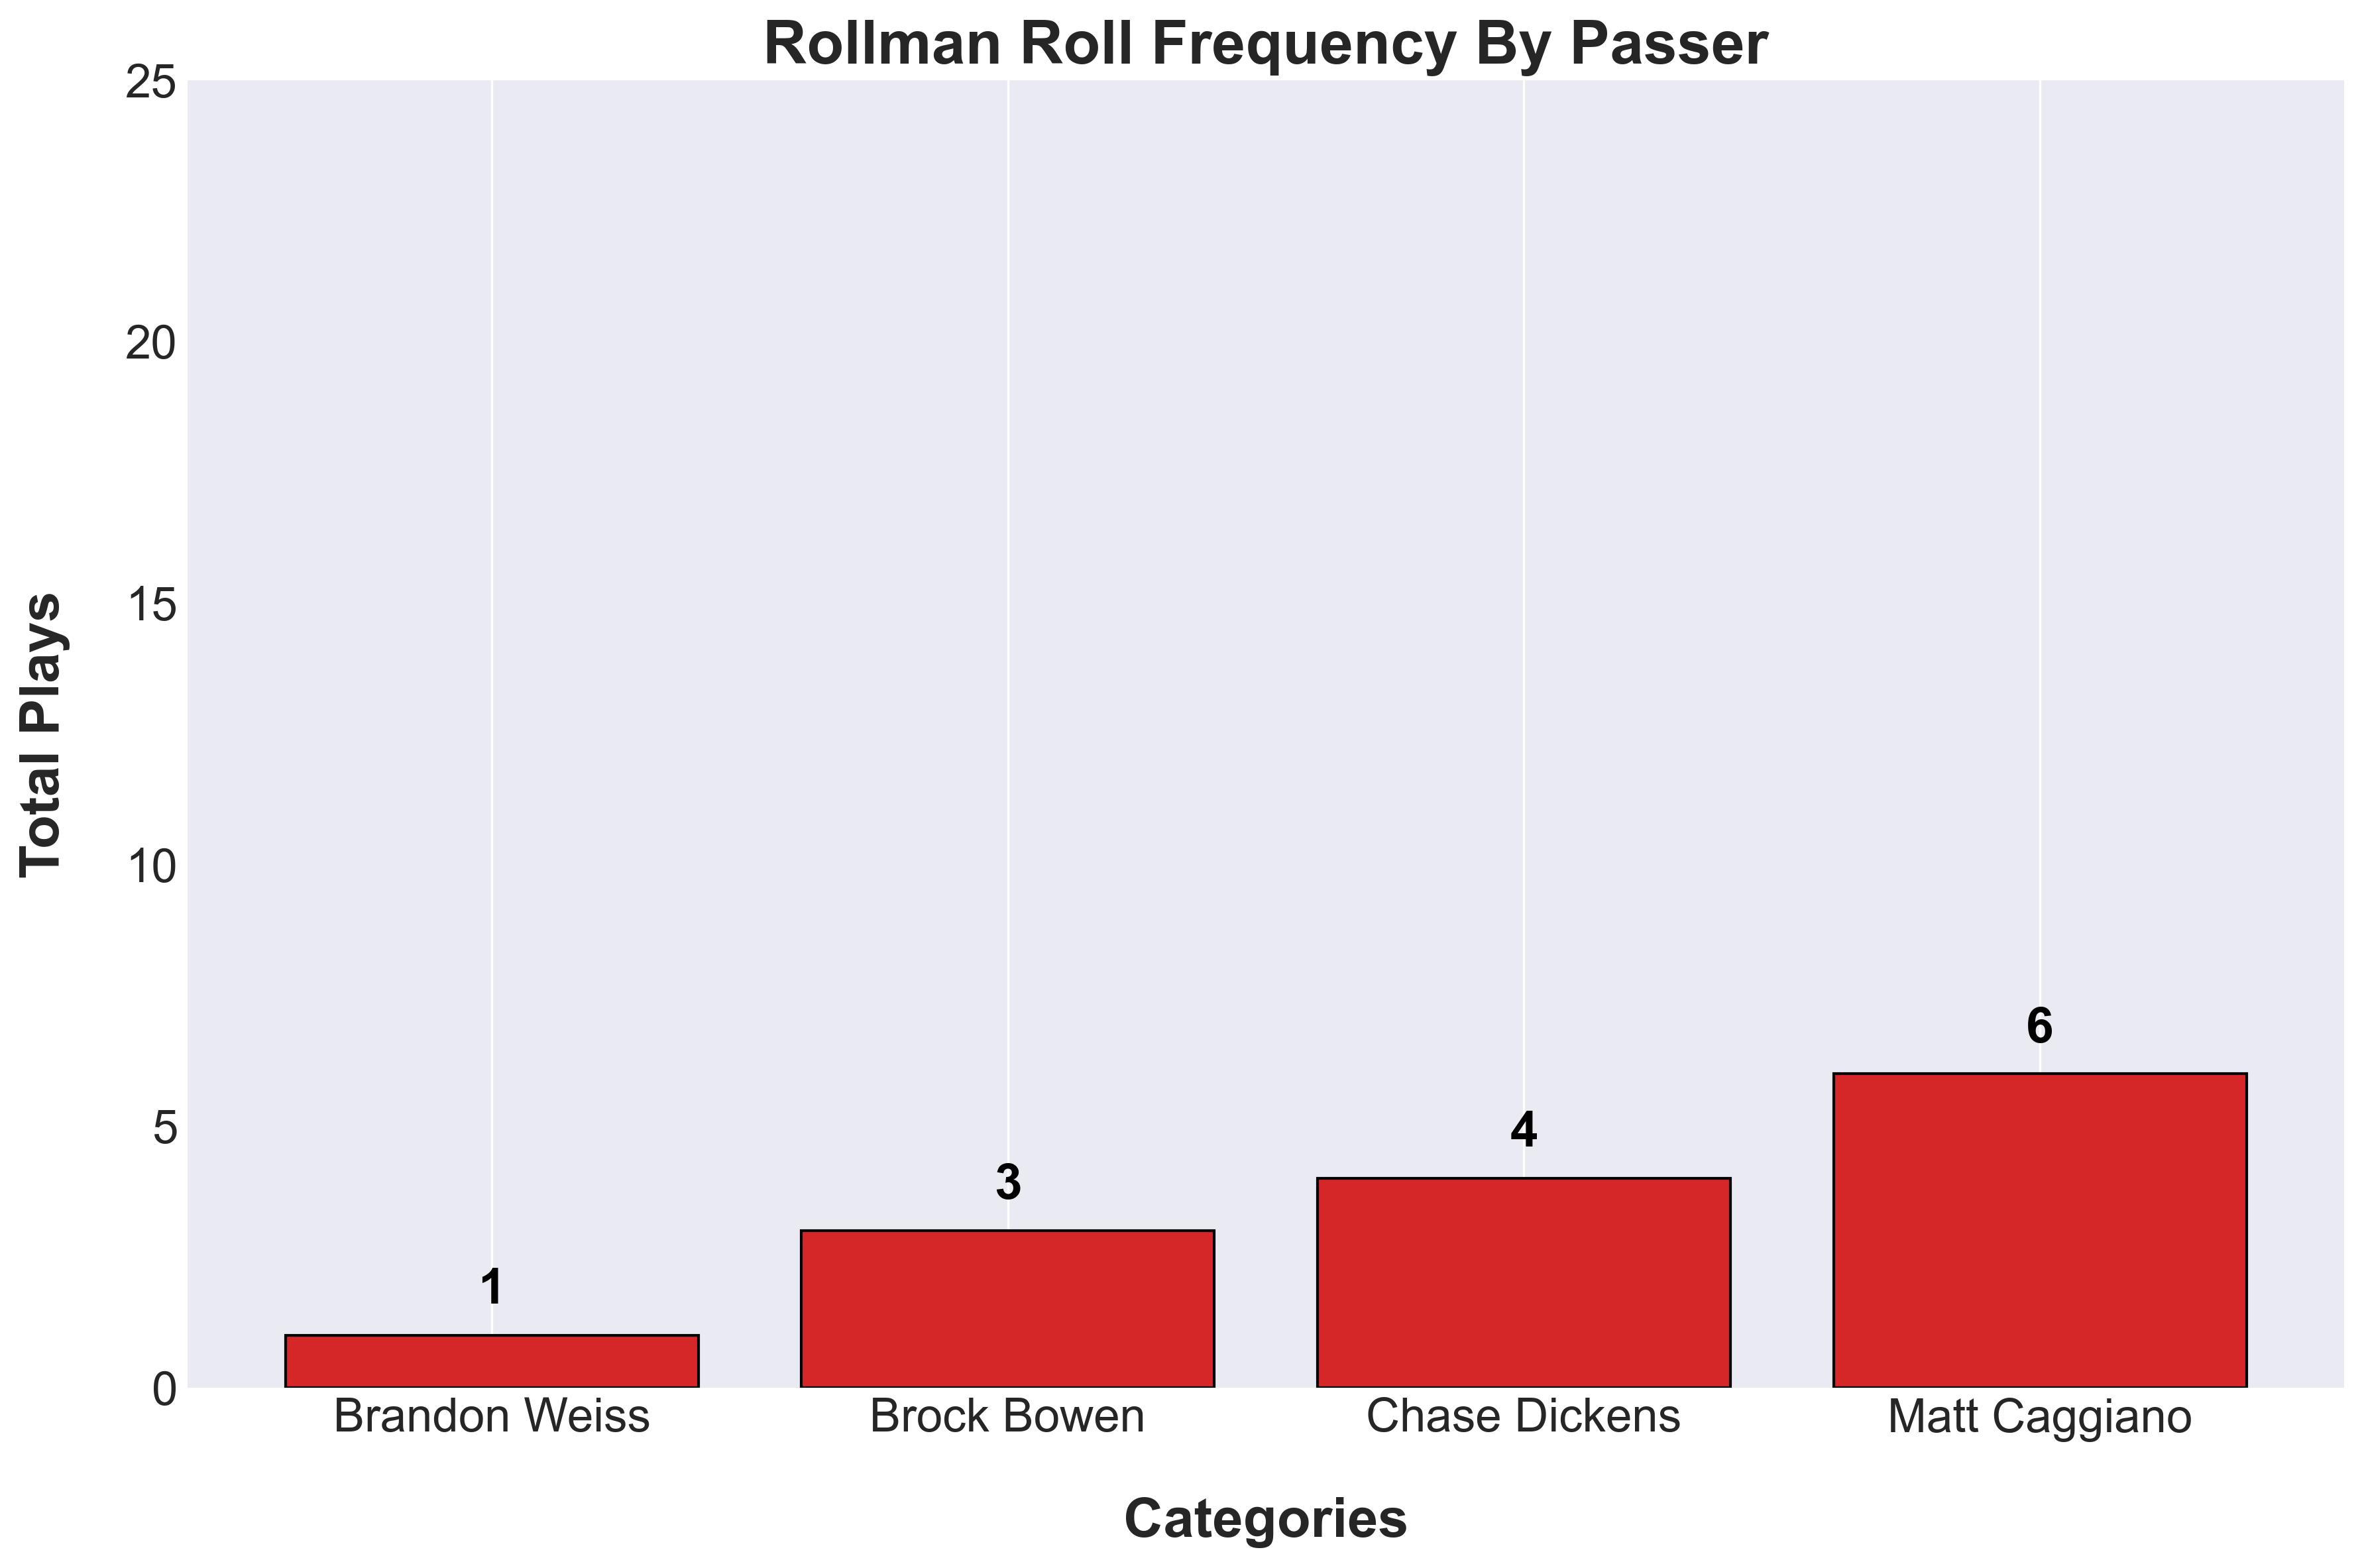
\includegraphics[width=\textwidth, height=.14\textheight]{images/Rollman_RollPlayer_Freq.png} % Adjust the width of the image to fit
    \end{minipage}
\end{table}

\vspace{-1em} % Add vertical space before the line (optional)
\hrule height 1pt width 1\textwidth % Adjust height and width
\vspace{1em} % Add vertical space after the line (optional)


% ----------------------
% Spot Up Visuals and Insights Section
% ----------------------
\subsection{Spot Ups}

\vspace{1em} % Add vertical space before the line (optional)
\hrule height 1pt width 1\textwidth % Adjust height and width
\vspace{1em} % Add vertical space after the line (optional)

\subsubsection{Spot Up Shot / Drive Statistics}

% All Spot up Statistics Table w/ room for insights
\begin{table}[H]
    \centering
    \begin{minipage}[t]{0.6\textwidth} % Left side (table) takes 85% of the width
        %\flushright
        \centering % Centering the title and the table
        \text{Total Spot Up Statistics} % Title above the table in bold
        \vskip .25em % Adds vertical space between title and table
        \scalebox{.85}{ % Scale the entire table down by half
            \scriptsize % Reduce the font size
            \begin{tabular}{
            >{\centering\arraybackslash}p{.75cm} 
            >{\centering\arraybackslash}p{.5cm} 
            >{\centering\arraybackslash}p{.5cm} 
            >{\centering\arraybackslash}p{.5cm}
            >{\centering\arraybackslash}p{.5cm} 
            >{\centering\arraybackslash}p{.5cm} 
            >{\centering\arraybackslash}p{.5cm} 
            >{\centering\arraybackslash}p{.5cm}
            >{\centering\arraybackslash}p{.5cm} 
            >{\centering\arraybackslash}p{.5cm}
            >{\centering\arraybackslash}p{.5cm} 
            >{\centering\arraybackslash}p{.5cm}}% Adjust column widths
            \toprule
            \textbf{Plays} &
            \textbf{3PA} &
            \textbf{3PM} &
            \textbf{3P\%} & 
            \textbf{2PA} & 
            \textbf{2PM} & 
            \textbf{2P\%} & 
            \textbf{MiA} & 
            \textbf{MiM} &
            \textbf{Mi\%} &
            \textbf{TO} &
            \textbf{Foul} \\
            \midrule
            
                
            
                
            
                
            
                
            
                
            
                
            
                
            
                
            
                
            
                
            
                
            
                
            
                
            
                
            
                
            
                
                    40 & 9 & 2 &
                    22.22 & 
                    26 & 6 &
                    23.08 &
                    20 & 4 &
                    20.0 &
                    3 & 2 \\
                
            
                
            
                
            
                
            
                
            
                
            
                
            

            \bottomrule
            \end{tabular}
        }
    \end{minipage}
\end{table}

\vspace{0em} % Add vertical space before the line (optional)
%\hrule height 1pt width 1\textwidth % Adjust height and width
\vspace{-1em} % Add vertical space after the line (optional)

% Spot up Stats for Jumpers vs Drives
\begin{table}[H]
    \raisebox{3em}{ % Adjust this value to shift the tables vertically
    \begin{minipage}[t]{0.6\textwidth} % Left side (table) takes 85% of the width
        \flushleft
        \centering % Centering the title and the table
        \text{Spot Up Statistics} % Title above the table in bold
        \vskip .25em % Adds vertical space between title and table
        \scalebox{.6}{ % Scale the entire table down by half
            \renewcommand{\arraystretch}{1.4} % Adjust the number to increase or decrease row spacing
            \begin{tabular}{
            >{\centering\arraybackslash}p{1.75cm} 
            >{\centering\arraybackslash}p{.75cm} 
            >{\centering\arraybackslash}p{.75cm} 
            >{\centering\arraybackslash}p{.75cm} 
            >{\centering\arraybackslash}p{.75cm}
            >{\centering\arraybackslash}p{.75cm} 
            >{\centering\arraybackslash}p{.75cm} 
            >{\centering\arraybackslash}p{.75cm} 
            >{\centering\arraybackslash}p{.75cm}
            >{\centering\arraybackslash}p{.75cm} 
            >{\centering\arraybackslash}p{.75cm}
            >{\centering\arraybackslash}p{.75cm} 
            >{\centering\arraybackslash}p{.75cm}}% Adjust column widths
            \toprule
            {\scriptsize \textbf{PlayType}} &
            {\scriptsize \textbf{Plays}} &
            {\scriptsize \textbf{3PA}} &
            {\scriptsize \textbf{3PM}} &
            {\scriptsize \textbf{3P\%}} & 
            {\scriptsize \textbf{2PA}} & 
            {\scriptsize \textbf{2PM}} & 
            {\scriptsize \textbf{2P\%}} & 
            {\scriptsize \textbf{MiA}} & 
            {\scriptsize \textbf{MiM}} &
            {\scriptsize \textbf{Mi\%}} &
            {\scriptsize \textbf{TO}} &
            {\scriptsize \textbf{Foul}} \\
            \midrule
            
                
            
                
            
                
            
                
            
                
            
                
            
                
            
                
            
                
            
                
            
                
            
                
            
                
            
                
            
                
            
                
            
                
            
                
                    Jumpshot & 23 & 9 & 2 &
                    22.22 & 
                    14 & 1 &
                    7.14 &
                    14 & 1 &
                    7.14 &
                    0 & 0 \\
                
            
                
                    Drive & 17 & 0 & 0 &
                    - & 
                    12 & 5 &
                    41.67 &
                    6 & 3 &
                    50.0 &
                    3 & 2 \\
                
            
                
            
                
            
                
            


            \bottomrule
        \end{tabular}
        } % End of \scalebox
    \end{minipage}
    } % End of raisebox, closing the adjustment
    \hfill % This adds some flexible space between the table and the image
    \begin{minipage}[c]{0.35\textwidth} % Right side (image) takes 10% of the width
        \flushright
        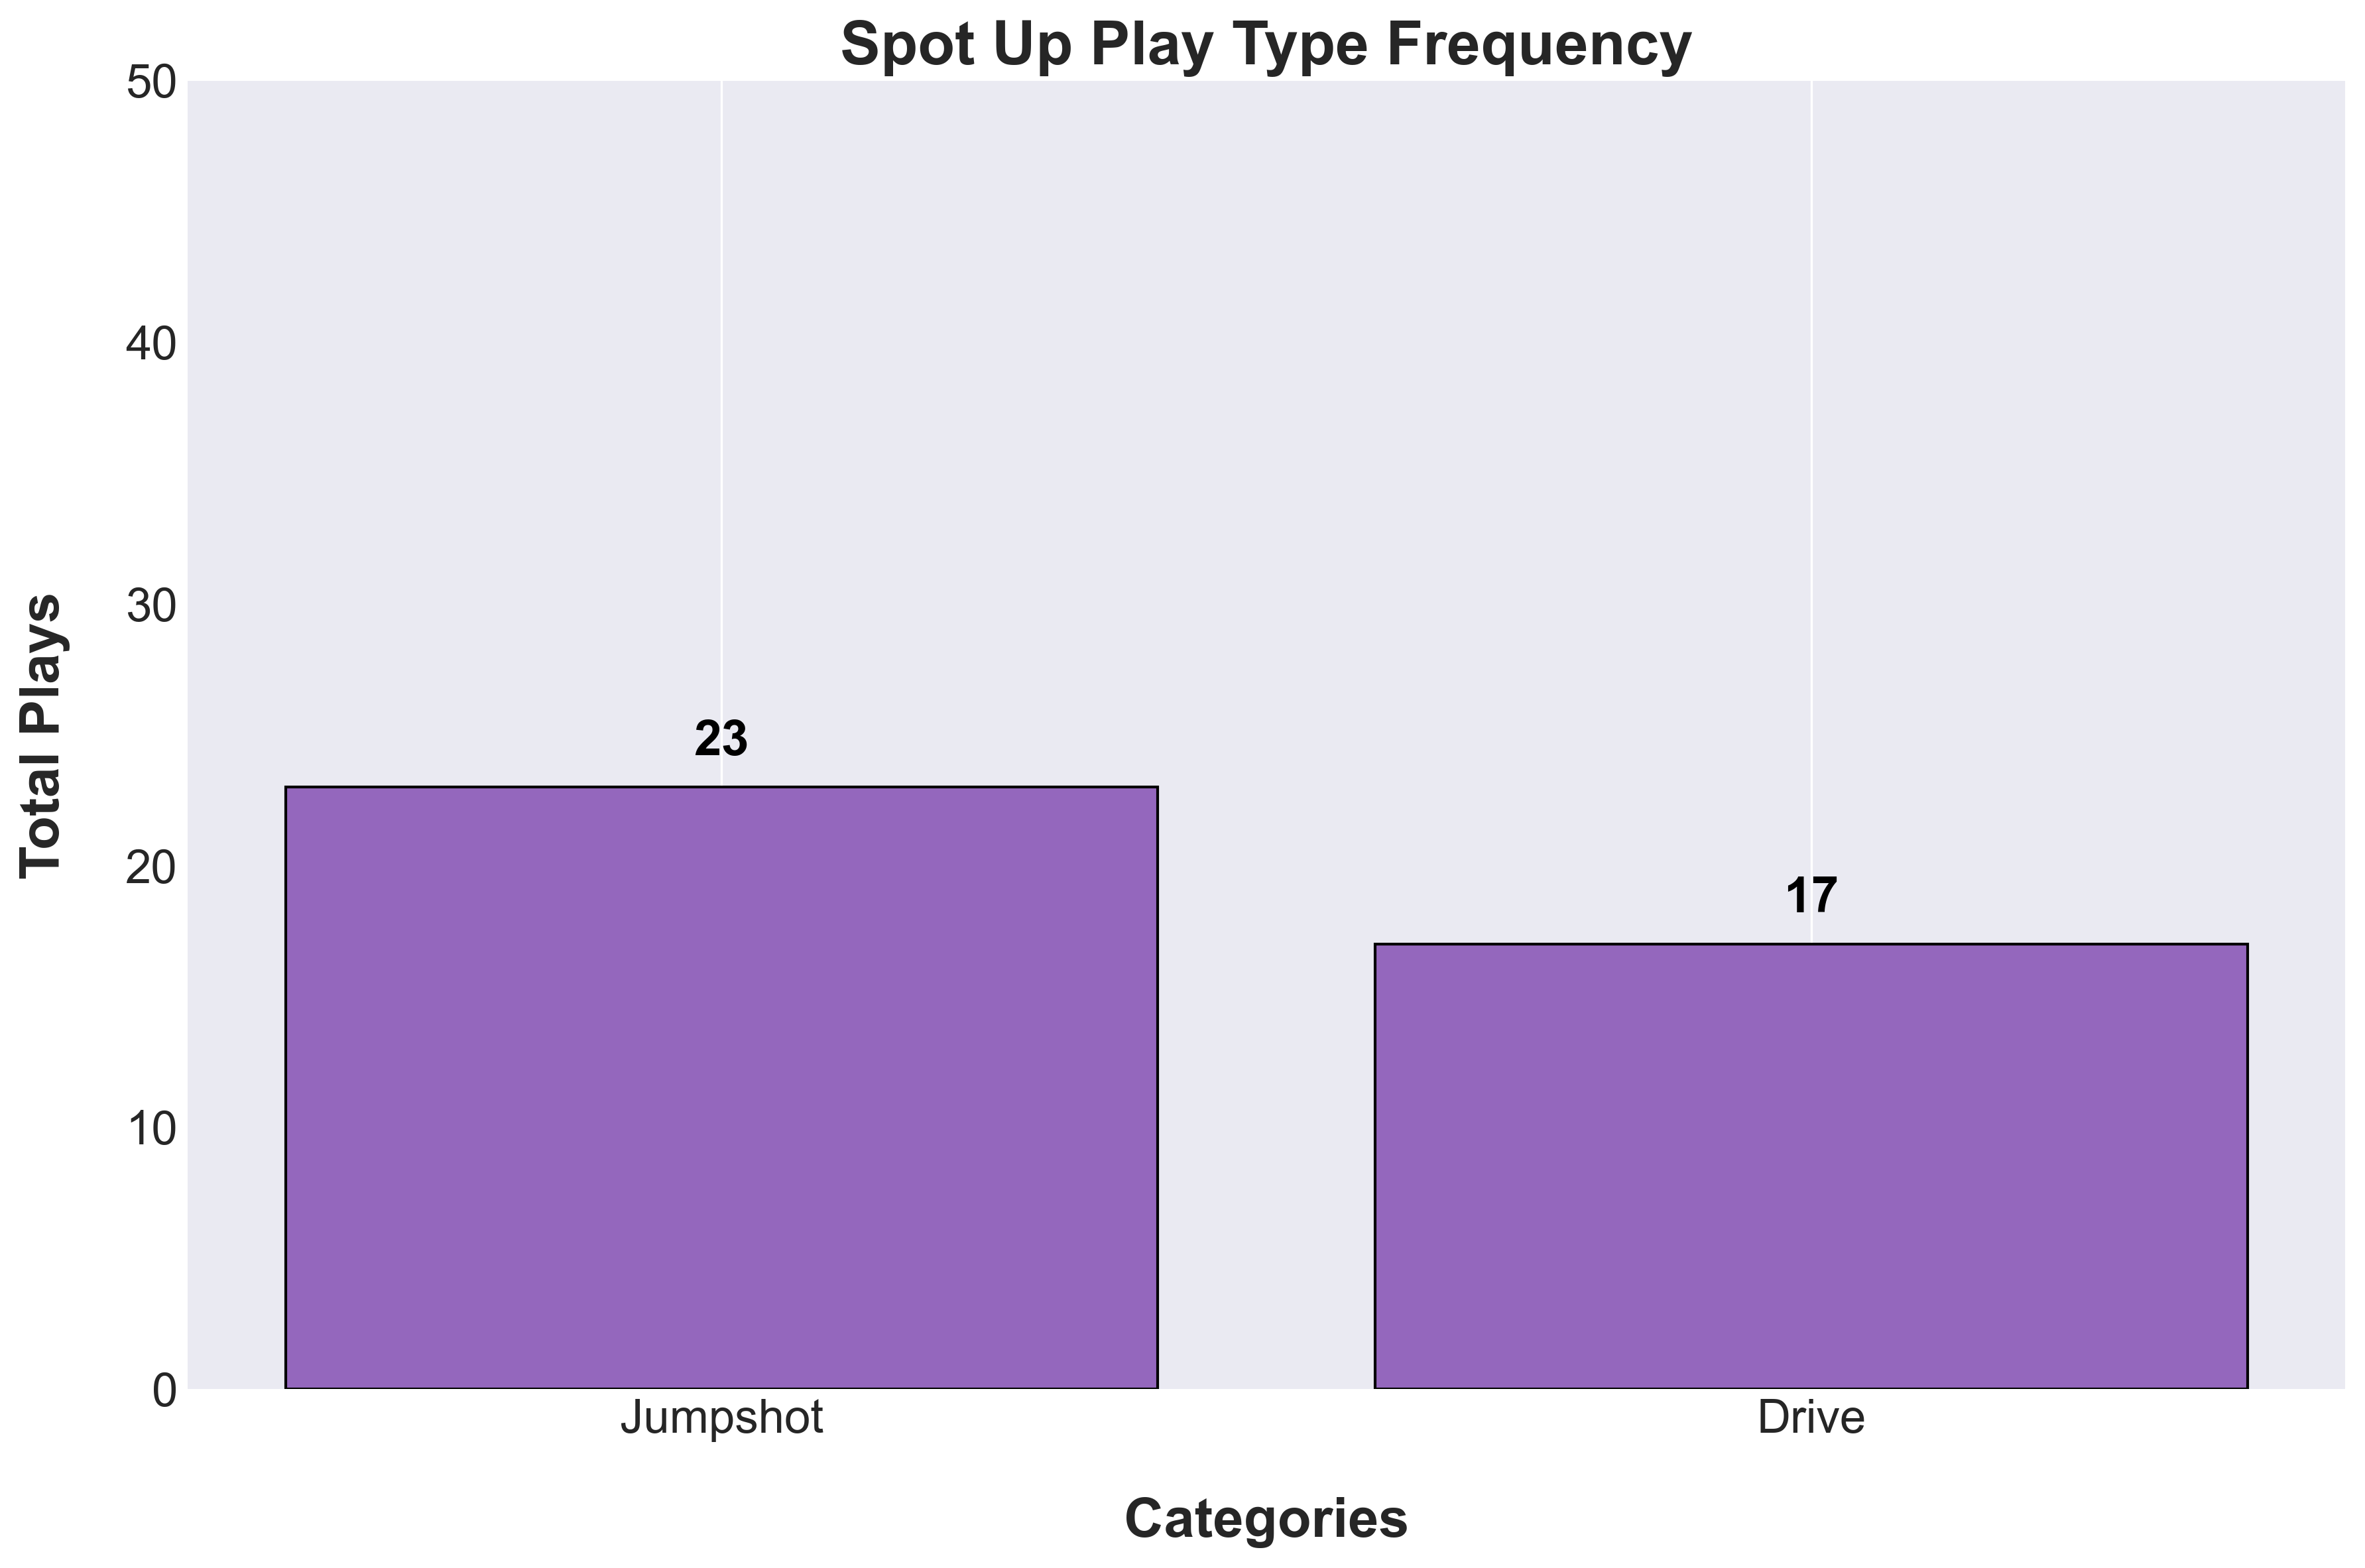
\includegraphics[width=\textwidth, height=.14\textheight]{images/SpotUp_PlayType_Freq.png} % Adjust the width of the image to fit
    \end{minipage}
\end{table}

\vspace{-1em} % Add vertical space before the line (optional)
%\hrule height 1pt width 1\textwidth % Adjust height and width
\vspace{-1em} % Add vertical space after the line (optional)

% Spot up Drives, Left vs Right vs Straight
\begin{table}[H]
    \raisebox{3.5em}{ % Adjust this value to shift the tables vertically
    \centering
    \begin{minipage}[t]{0.6\textwidth} % Left side (table) takes 85% of the width
        \centering % Centering the title and the table
        \text{Drive Direction Statistics} % Title above the table in bold
        \vskip .25em % Adds vertical space between title and table
        \scalebox{.9}{ % Scale the entire table down by half
            \scriptsize % Reduce the font size
            \renewcommand{\arraystretch}{1.4} % Adjust the number to increase or decrease row spacing
            \begin{tabular}{
            >{\centering\arraybackslash}p{1.5cm} 
            >{\centering\arraybackslash}p{.75cm} 
            >{\centering\arraybackslash}p{.5cm} 
            >{\centering\arraybackslash}p{.5cm} 
            >{\centering\arraybackslash}p{.5cm} 
            >{\centering\arraybackslash}p{.5cm}
            >{\centering\arraybackslash}p{.5cm} 
            >{\centering\arraybackslash}p{.5cm}
            >{\centering\arraybackslash}p{.5cm} 
            >{\centering\arraybackslash}p{.5cm}}% Adjust column widths
            \toprule
            \textbf{Direction} & \textbf{Plays} & \textbf{2PA} & \textbf{2PM} & 
            \textbf{2P\%} & \textbf{MiA} & \textbf{MiM} &
            \textbf{Mi\%} & \textbf{TO} & \textbf{Foul} \\
            \midrule
            
                
            
                
            
                
            
                
            
                
            
                
            
                
            
                
            
                
            
                
            
                
            
                
            
                
            
                
            
                
            
                
            
                
            
                
            
                
            
                
                    Left & 6 & 4 & 2 &
                    50.0 &
                    2 & 1 &
                    50.0 &
                    2 & 0 \\
                
            
                
                    Right & 9 & 6 & 2 &
                    33.33 &
                    2 & 1 &
                    50.0 &
                    1 & 2 \\
                
            
                
                    Straight & 2 & 2 & 1 &
                    50.0 &
                    2 & 1 &
                    50.0 &
                    0 & 0 \\
                
            


            \bottomrule
        \end{tabular}
        } % End of \scalebox
    \end{minipage}
    } % End of raisebox, closing the adjustment
    \hfill
    \begin{minipage}[c]{0.35\textwidth} % Right side (image) takes 10% of the width
        \flushright
        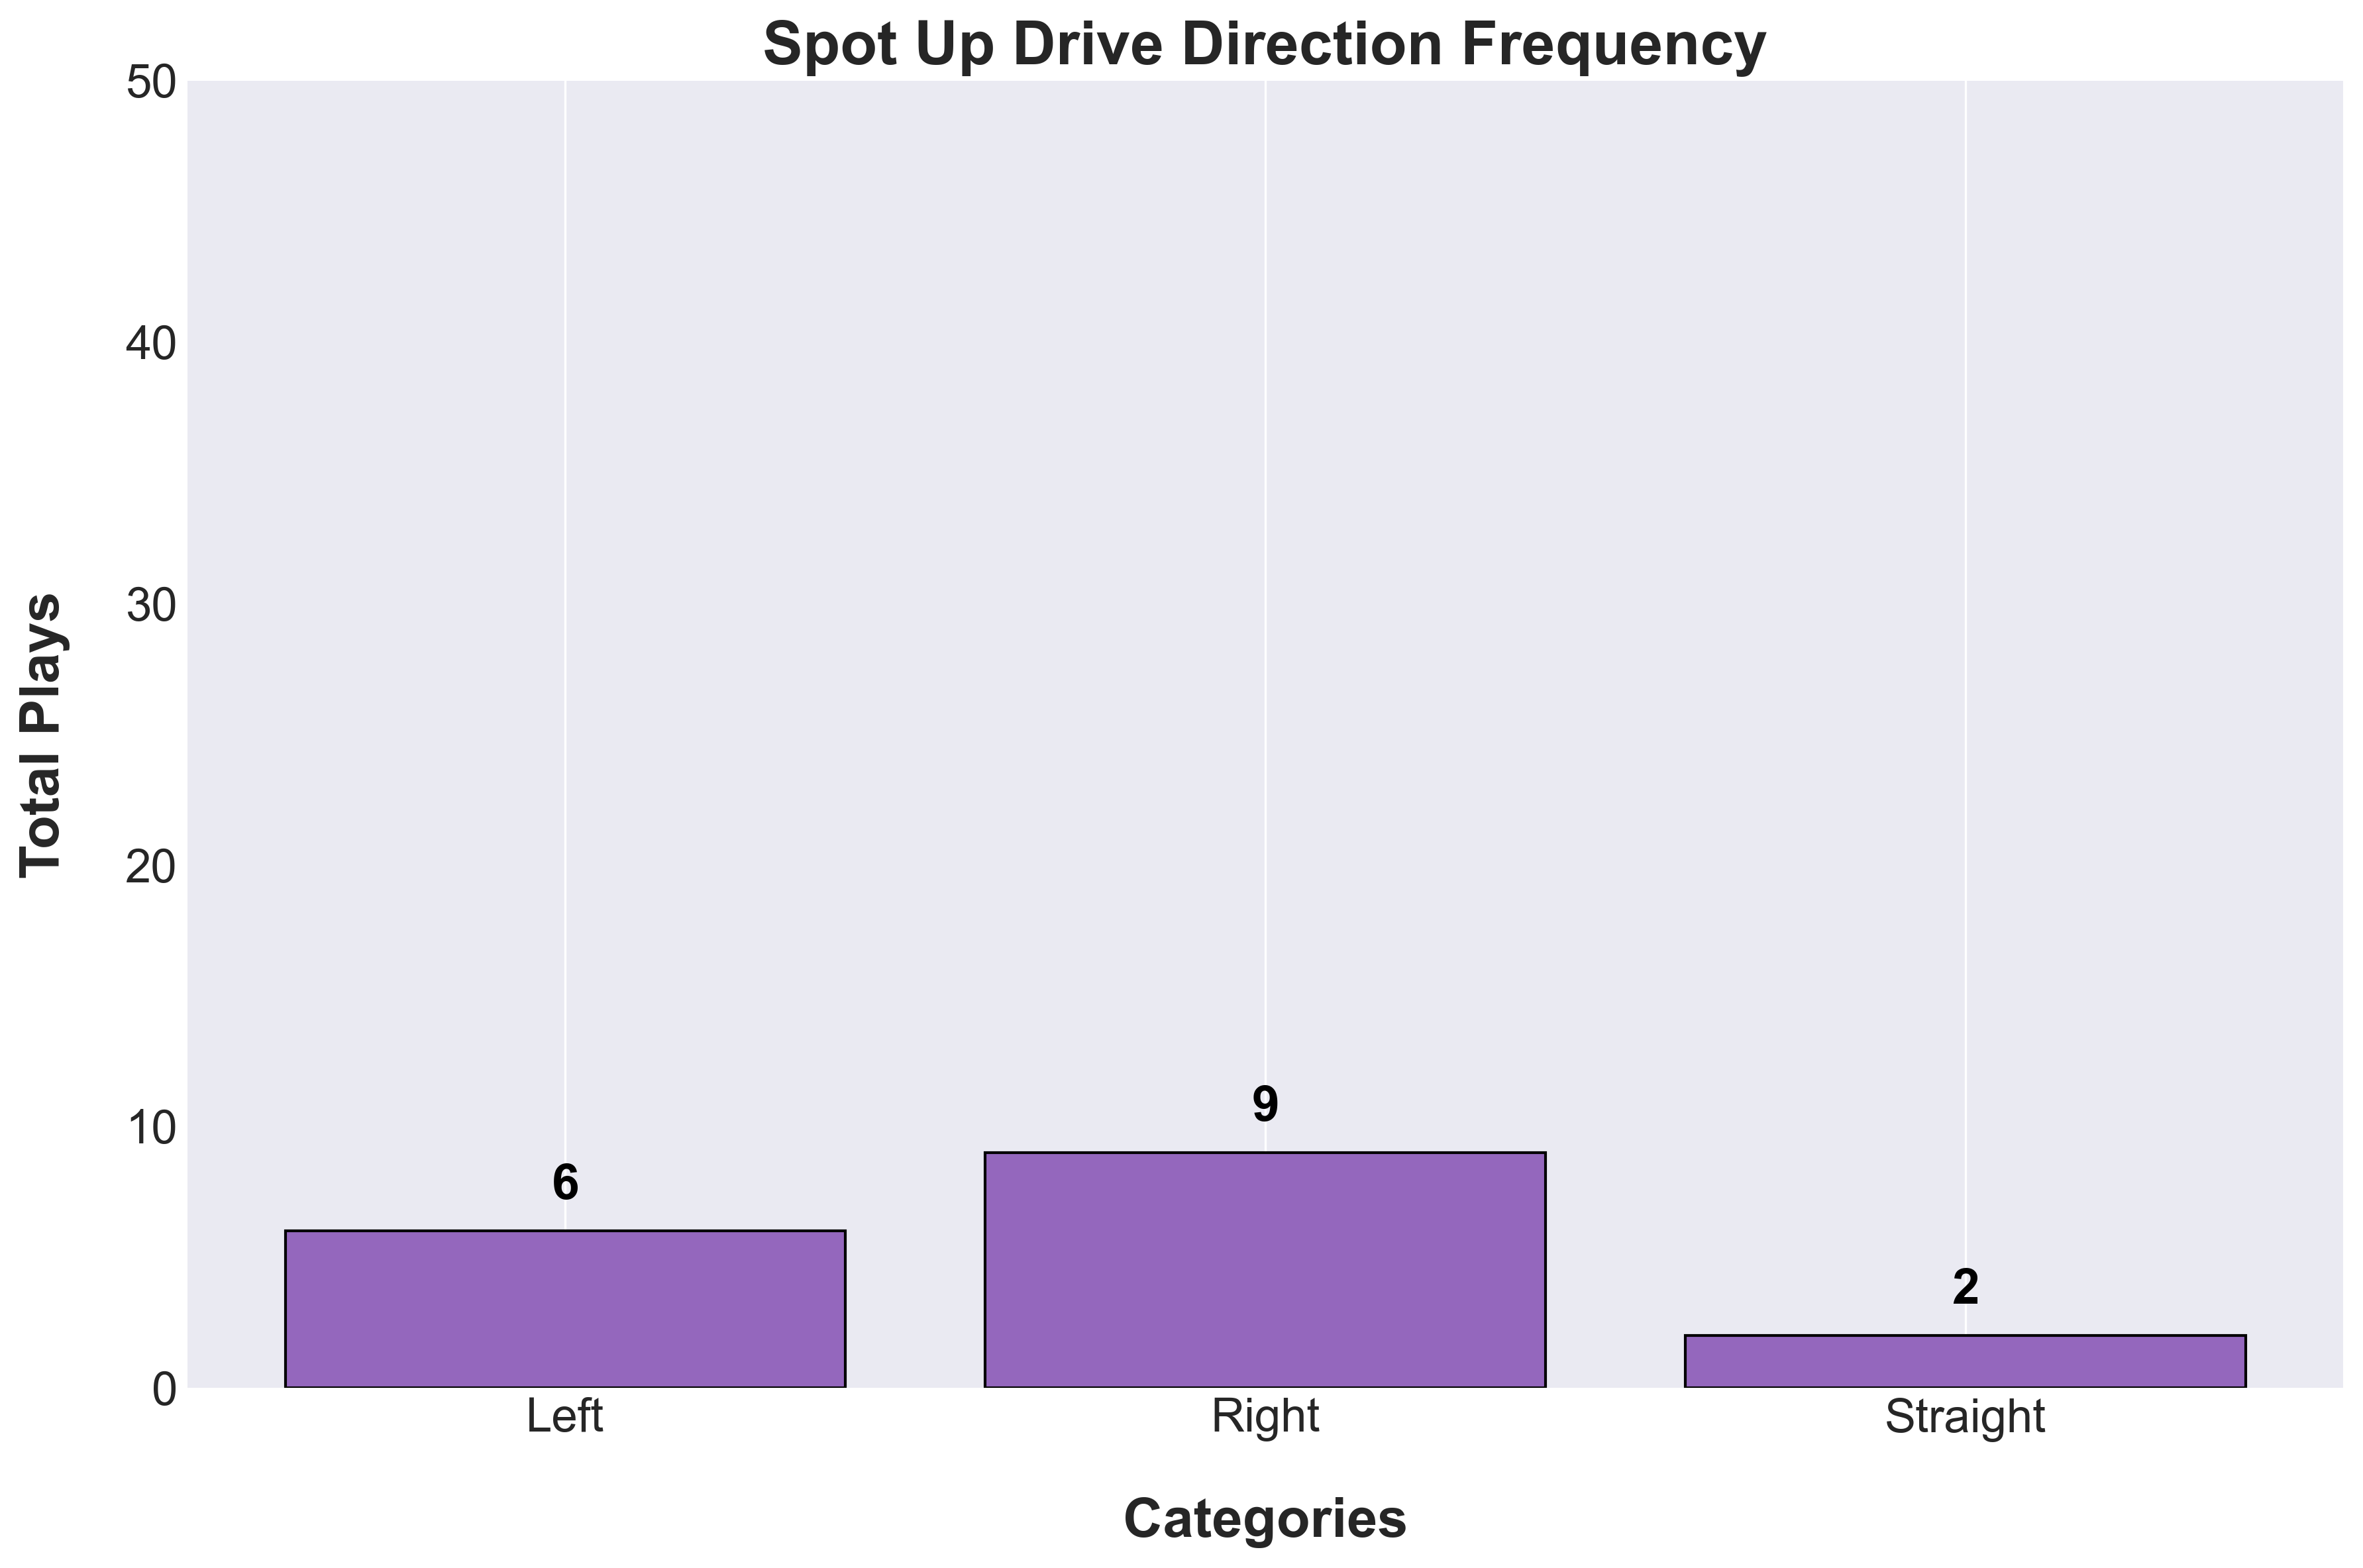
\includegraphics[width=\textwidth, height=.14\textheight]{images/SpotUp_DriveDirection_Freq.png} % Adjust the width of the image to fit
    \end{minipage}
    
\end{table}

\vspace{-1em} % Add vertical space before the line (optional)
\hrule height 1pt width 1\textwidth % Adjust height and width
\vspace{1 em} % Add vertical space after the line (optional)

\subsubsection{Stats on where Player gets Spot Ups from}

% Images of where they receive the ball SU Drives / Shots
\begin{table}[H]
    \centering
    \begin{minipage}[c]{0.45\textwidth} % First image minipage (45% of text width)
        \centering
        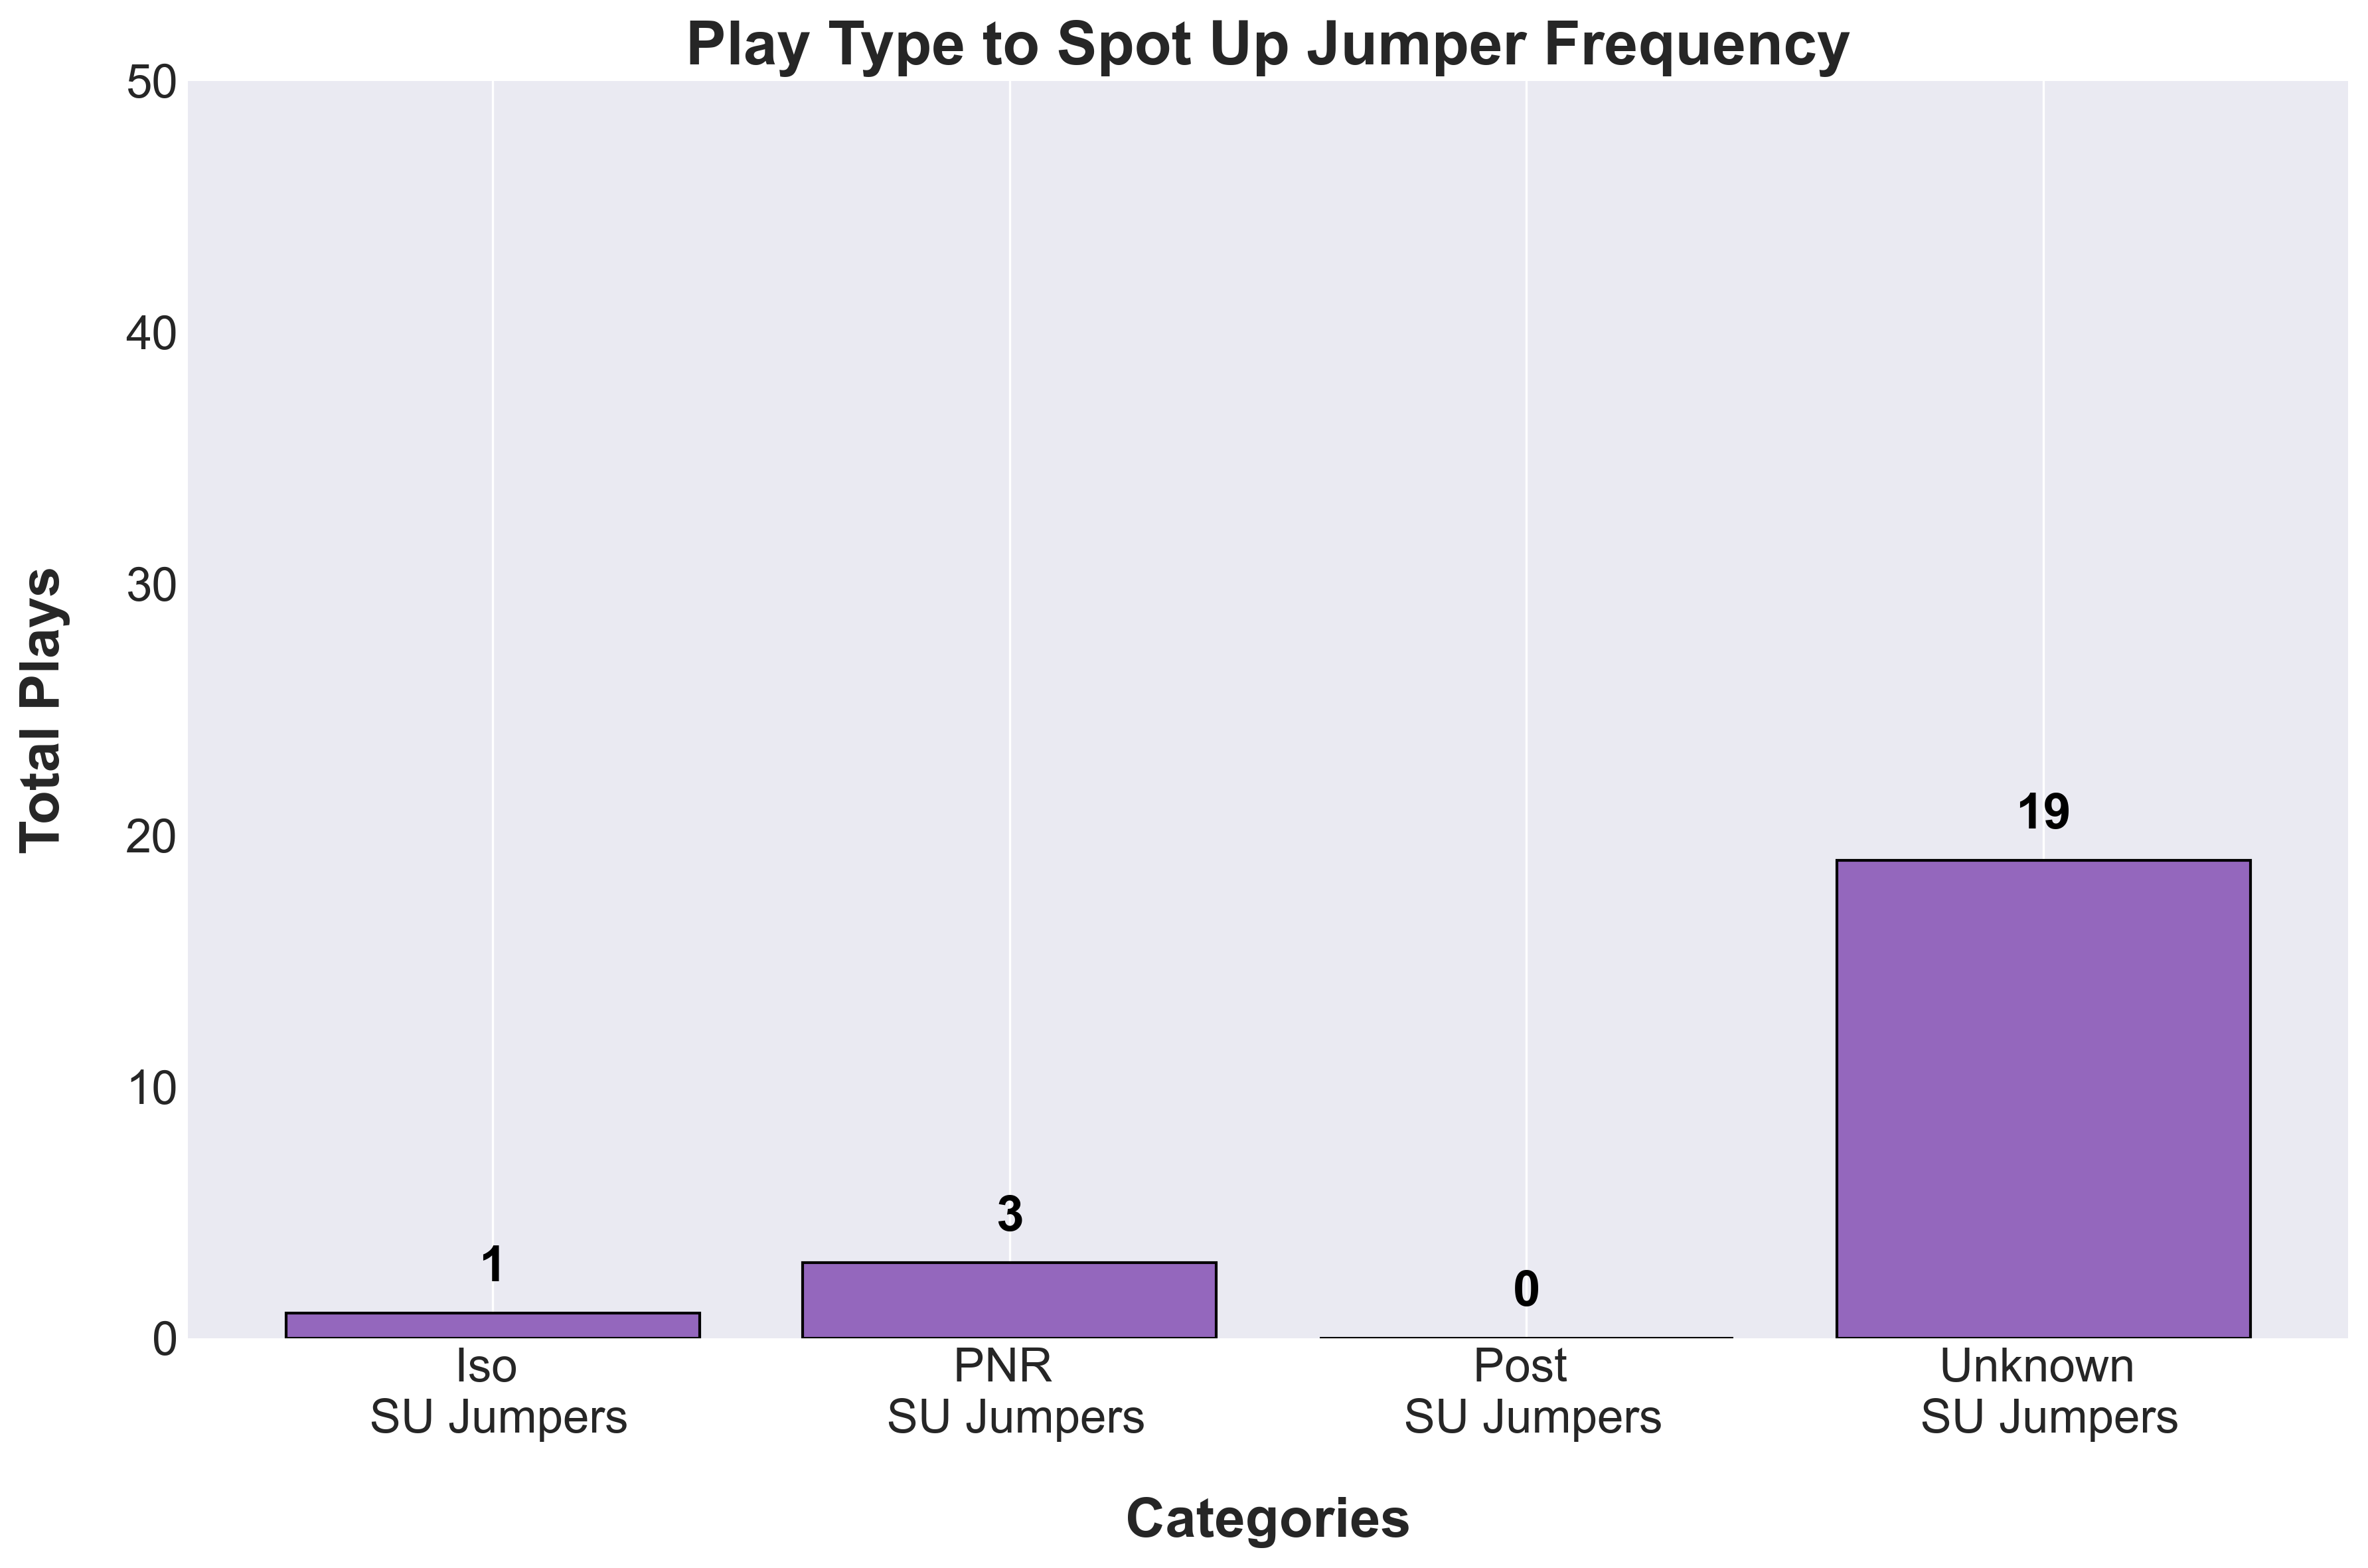
\includegraphics[width=.8\textwidth, height=0.15\textheight]{images/SpotUp_PlayTypeShots_Freq.png} % Adjust image to fill the minipage but scale height to 3/4
    \end{minipage}
    \hfill % Flexible space between images
    \begin{minipage}[c]{0.45\textwidth} % Second image minipage (45% of text width)
        \centering
        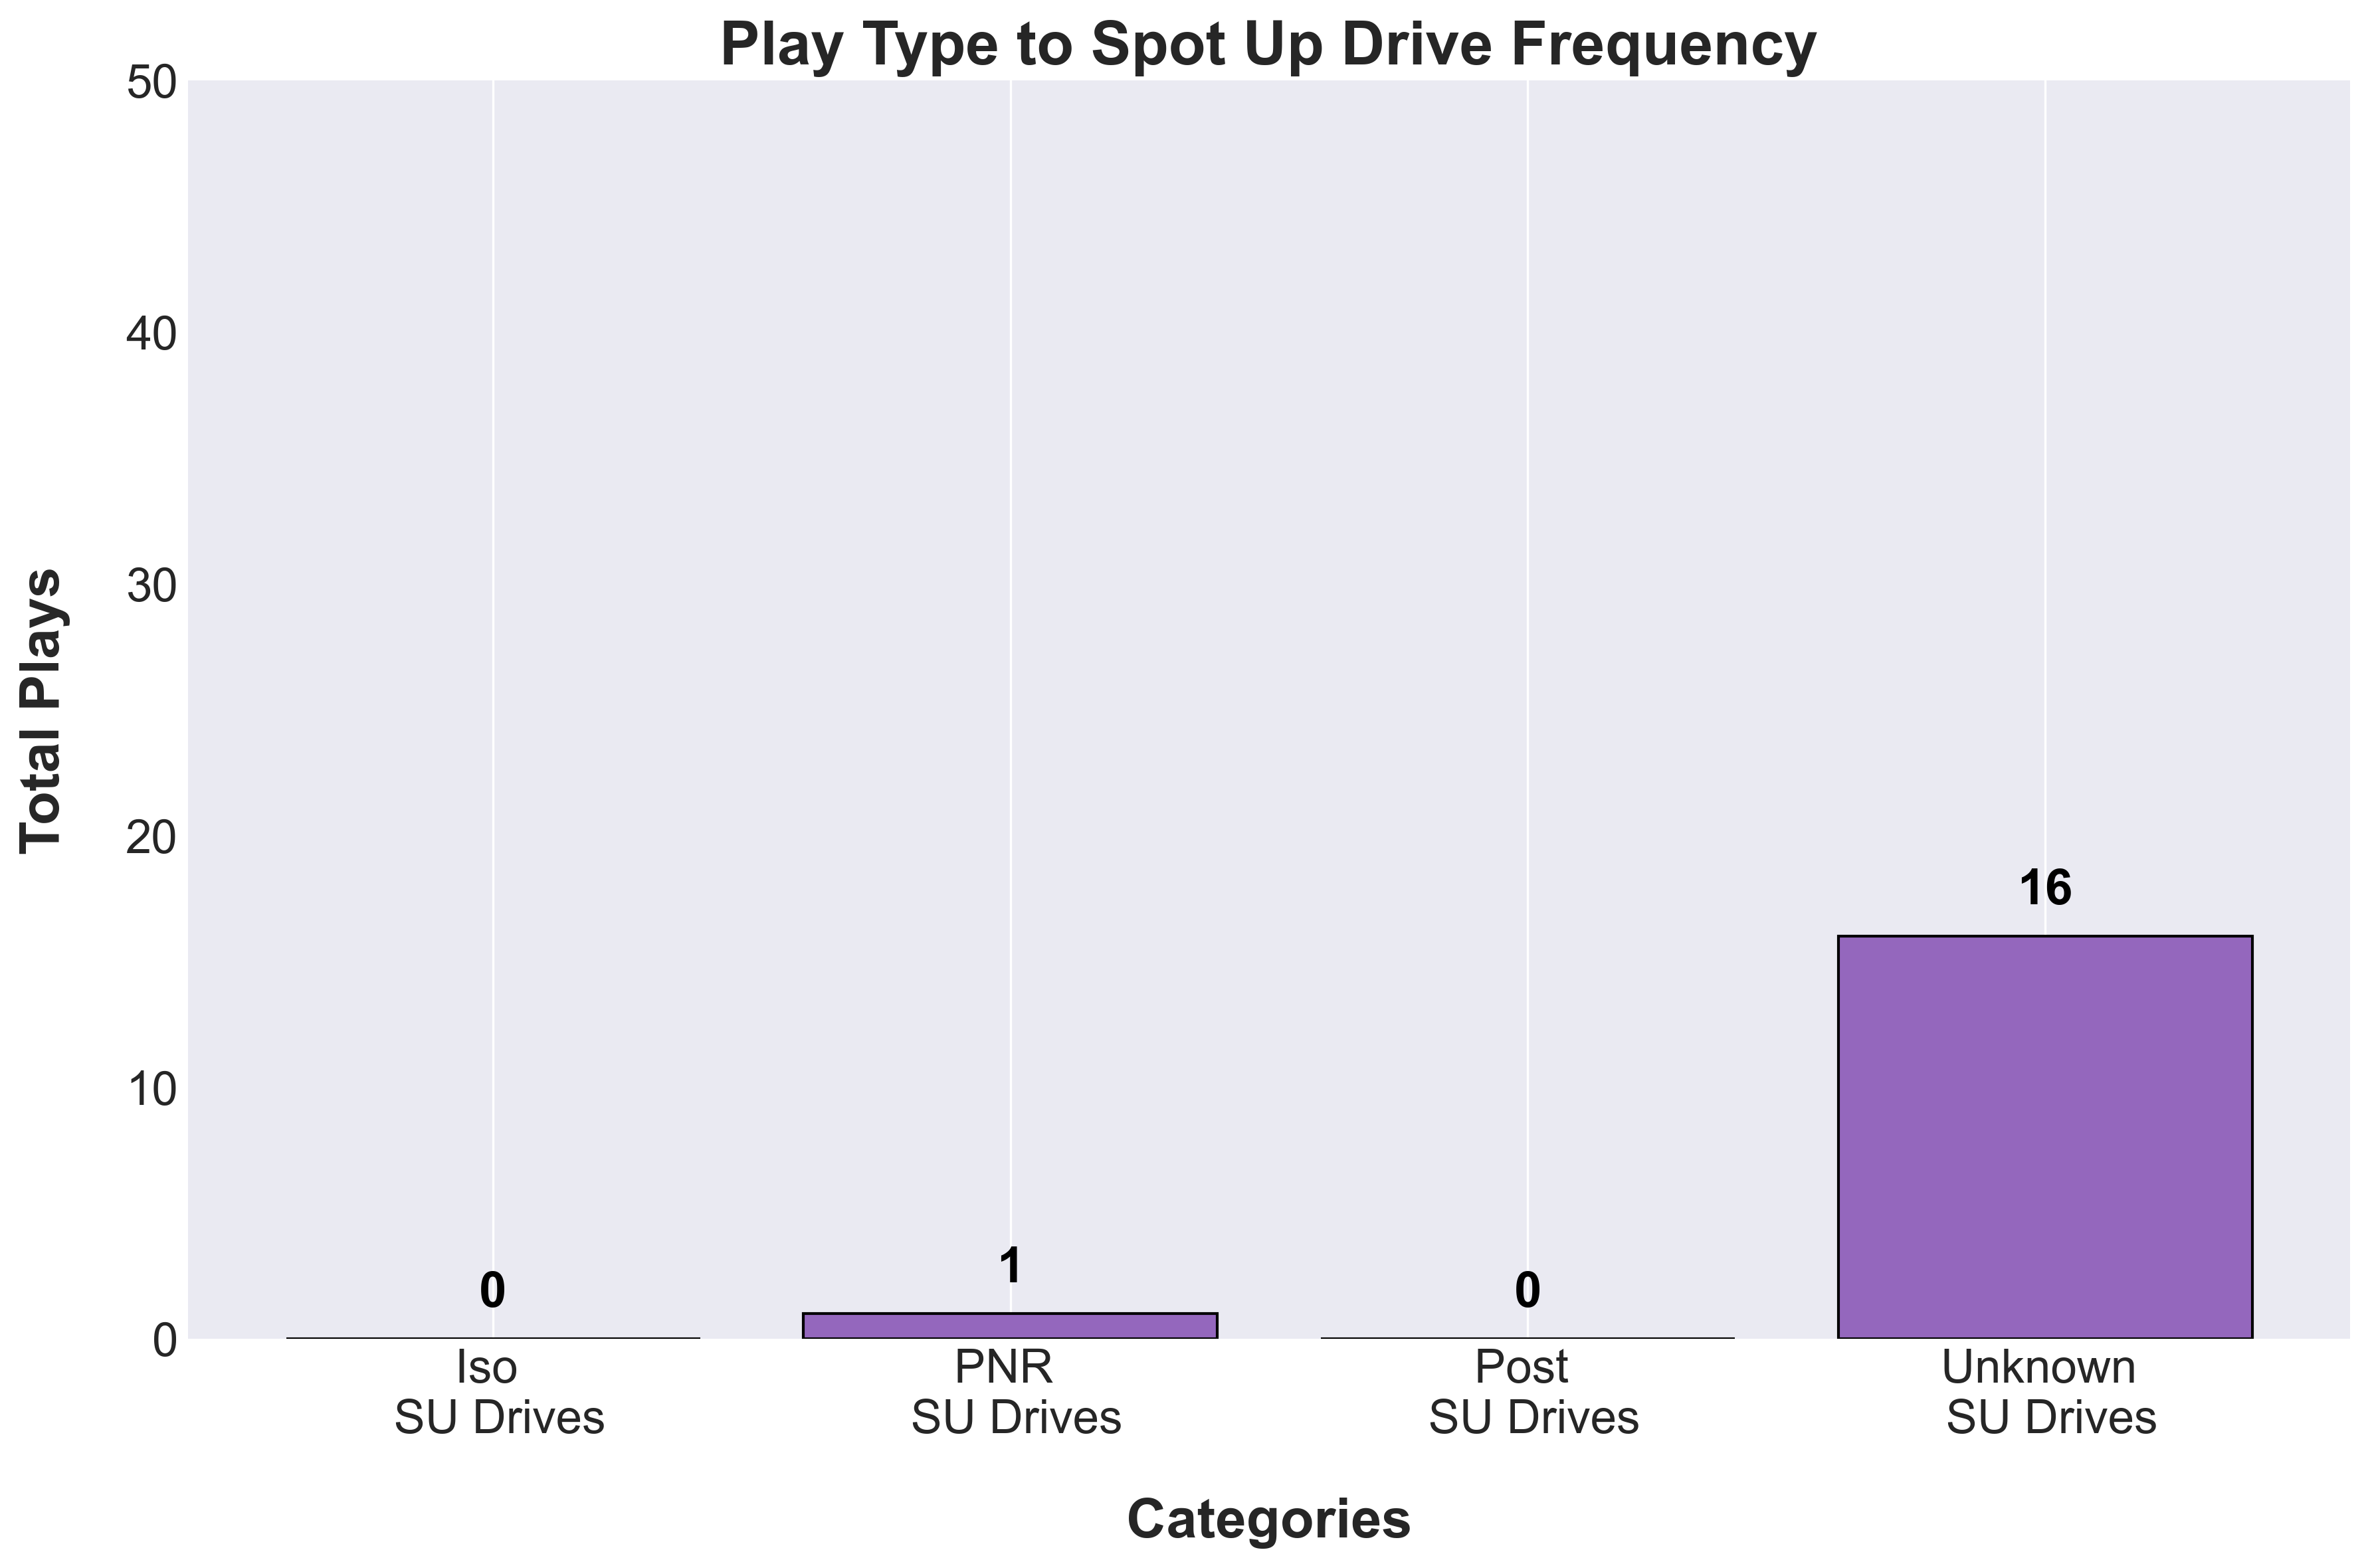
\includegraphics[width=.8\textwidth, height=0.15\textheight]{images/SpotUp_PlayTypeDrives_Freq.png} % Adjust image to fill the minipage but scale height to 3/4
    \end{minipage}
\end{table}

\vspace{-1em} % Add vertical space before the line (optional)
\vspace{-1em} % Add vertical space after the line (optional)

% Tables of where they receive the ball SU Drives / Shots
\begin{table}[H]
    \centering
    \raisebox{-1.5em}{
    \begin{minipage}[t]{0.45\textwidth} % Left table minipage
        \centering
        {\small \text{Different Playtype to Jumpshot Statistics}} % Center the title
        \vskip .25em % Adds vertical space between title and table
        \scalebox{.7}{ % Scale the entire table
            \scriptsize % Reduce the font size
            \renewcommand{\arraystretch}{1.3} % Adjust the number to increase or decrease row spacing
            \begin{tabular}{
            >{\centering\arraybackslash}p{1.25cm} 
            >{\centering\arraybackslash}p{.75cm} 
            >{\centering\arraybackslash}p{.5cm} 
            >{\centering\arraybackslash}p{.5cm}
            >{\centering\arraybackslash}p{.5cm} 
            >{\centering\arraybackslash}p{.5cm} 
            >{\centering\arraybackslash}p{.5cm}
            >{\centering\arraybackslash}p{.75cm}
            >{\centering\arraybackslash}p{.5cm} 
            >{\centering\arraybackslash}p{.5cm}}
            \toprule
            \textbf{PlayType} & \textbf{Plays} & \textbf{3PA} & \textbf{3PM} & \textbf{3P\%}  & \textbf{MiA} & \textbf{MiM} & \textbf{Mi\%}  & \textbf{TO} & \textbf{Foul} \\
            \midrule
            
                
            
                
            
                
            
                
            
                
            
                
                    Iso & 1 & 0 & 0 &
                    - & 
                    1 & 0 &
                    0.0 &
                    0 & 0 \\
                
            
                
            
                
            
                
            
                
                    PNR & 3 & 1 & 1 &
                    100.0 & 
                    2 & 0 &
                    0.0 &
                    0 & 0 \\
                
            
                
            
                
            
                
            
                
            
                
            
                
            
                
            
                
            
                
            
                
            
                
            
                
            



            \bottomrule
        \end{tabular}
        }
    \end{minipage}
    \hfill % Flexible space between the two tables
    \begin{minipage}[t]{0.45\textwidth} % Right table minipage
        \centering
        {\small \text{Different Playtype to Drive Statistics}}% Center the title
        \vskip .25em % Adds vertical space between title and table
        \scalebox{.65}{ % Scale the entire table
            \scriptsize % Reduce the font size
            \renewcommand{\arraystretch}{1.3} % Adjust the number to increase or decrease row spacing
            \begin{tabular}{
            >{\centering\arraybackslash}p{1.25cm} 
            >{\centering\arraybackslash}p{.75cm} 
            >{\centering\arraybackslash}p{.5cm} 
            >{\centering\arraybackslash}p{.5cm}
            >{\centering\arraybackslash}p{.5cm} 
            >{\centering\arraybackslash}p{.5cm} 
            >{\centering\arraybackslash}p{.5cm}
            >{\centering\arraybackslash}p{.75cm}
            >{\centering\arraybackslash}p{.5cm} 
            >{\centering\arraybackslash}p{.5cm}}
            \toprule
            \textbf{PlayType} & \textbf{Plays} & \textbf{2PA} & \textbf{2PM} & \textbf{2P\%} & \textbf{MiA} & \textbf{MiM} & \textbf{Mi\%} & \textbf{TO} & \textbf{Foul} \\
            \midrule
            
                
            
                
            
                
            
                
            
                
            
                
            
                
            
                
                    PNR & 1 &
                    1 & 0 &
                    0.0 &
                    1 & 0 &
                    0.0 &
                    0 & 0 \\
                
            
                
            
                
            
                
            
                
            
                
            
                
            
                
            
                
            
                
            
                
            
                
            
                
            
                
            
                
            

            
            \bottomrule
        \end{tabular}
        }
    \end{minipage}
    }
\end{table}

\vspace{1em} % Add vertical space before the line (optional)
\vspace{-1em} % Add vertical space after the line (optional)

% Post -> Jumpshot Stats by Passer
\begin{table}[H]
    \raisebox{3em}{ % Adjust this value to shift the tables vertically
    \begin{minipage}[t]{0.6\textwidth} % Left side (table) takes 85% of the width
        \flushleft
        \centering % Centering the title and the table
        \text{Post - Jumpshot Stats by Passer} % Title above the table in bold
        \vskip .25em % Adds vertical space between title and table
        \scalebox{.6}{ % Scale the entire table down by half
            \renewcommand{\arraystretch}{1.4} % Adjust the number to increase or decrease row spacing
            \begin{tabular}{
            >{\centering\arraybackslash}p{3cm} 
            >{\centering\arraybackslash}p{.75cm} 
            >{\centering\arraybackslash}p{.75cm} 
            >{\centering\arraybackslash}p{.75cm} 
            >{\centering\arraybackslash}p{.75cm}
            >{\centering\arraybackslash}p{.75cm}
            >{\centering\arraybackslash}p{.75cm} 
            >{\centering\arraybackslash}p{.75cm}
            >{\centering\arraybackslash}p{.75cm} 
            >{\centering\arraybackslash}p{.75cm}}% Adjust column widths
            \toprule
            {\scriptsize \textbf{Player}} &
            {\scriptsize \textbf{Plays}} &
            {\scriptsize \textbf{3PA}} &
            {\scriptsize \textbf{3PM}} &
            {\scriptsize \textbf{3P\%}} & 
            {\scriptsize \textbf{MiA}} & 
            {\scriptsize \textbf{MiM}} &
            {\scriptsize \textbf{Mi\%}} &
            {\scriptsize \textbf{TO}} &
            {\scriptsize \textbf{Foul}} \\
            \midrule
            
                
            
                
            
                
            
                
            
                
            
                
            
                
            
                
            
                
            
                
            
                
            
                
            
                
            
                
            
                
                    
                
            
                
            
                
            
                
            
                
            
                
            
                
            
                
            

            \bottomrule
        \end{tabular}
        } % End of \scalebox
    \end{minipage}
    } % End of raisebox, closing the adjustment
    \hfill % This adds some flexible space between the table and the image
    \begin{minipage}[c]{0.35\textwidth} % Right side (image) takes 10% of the width
        \flushright
        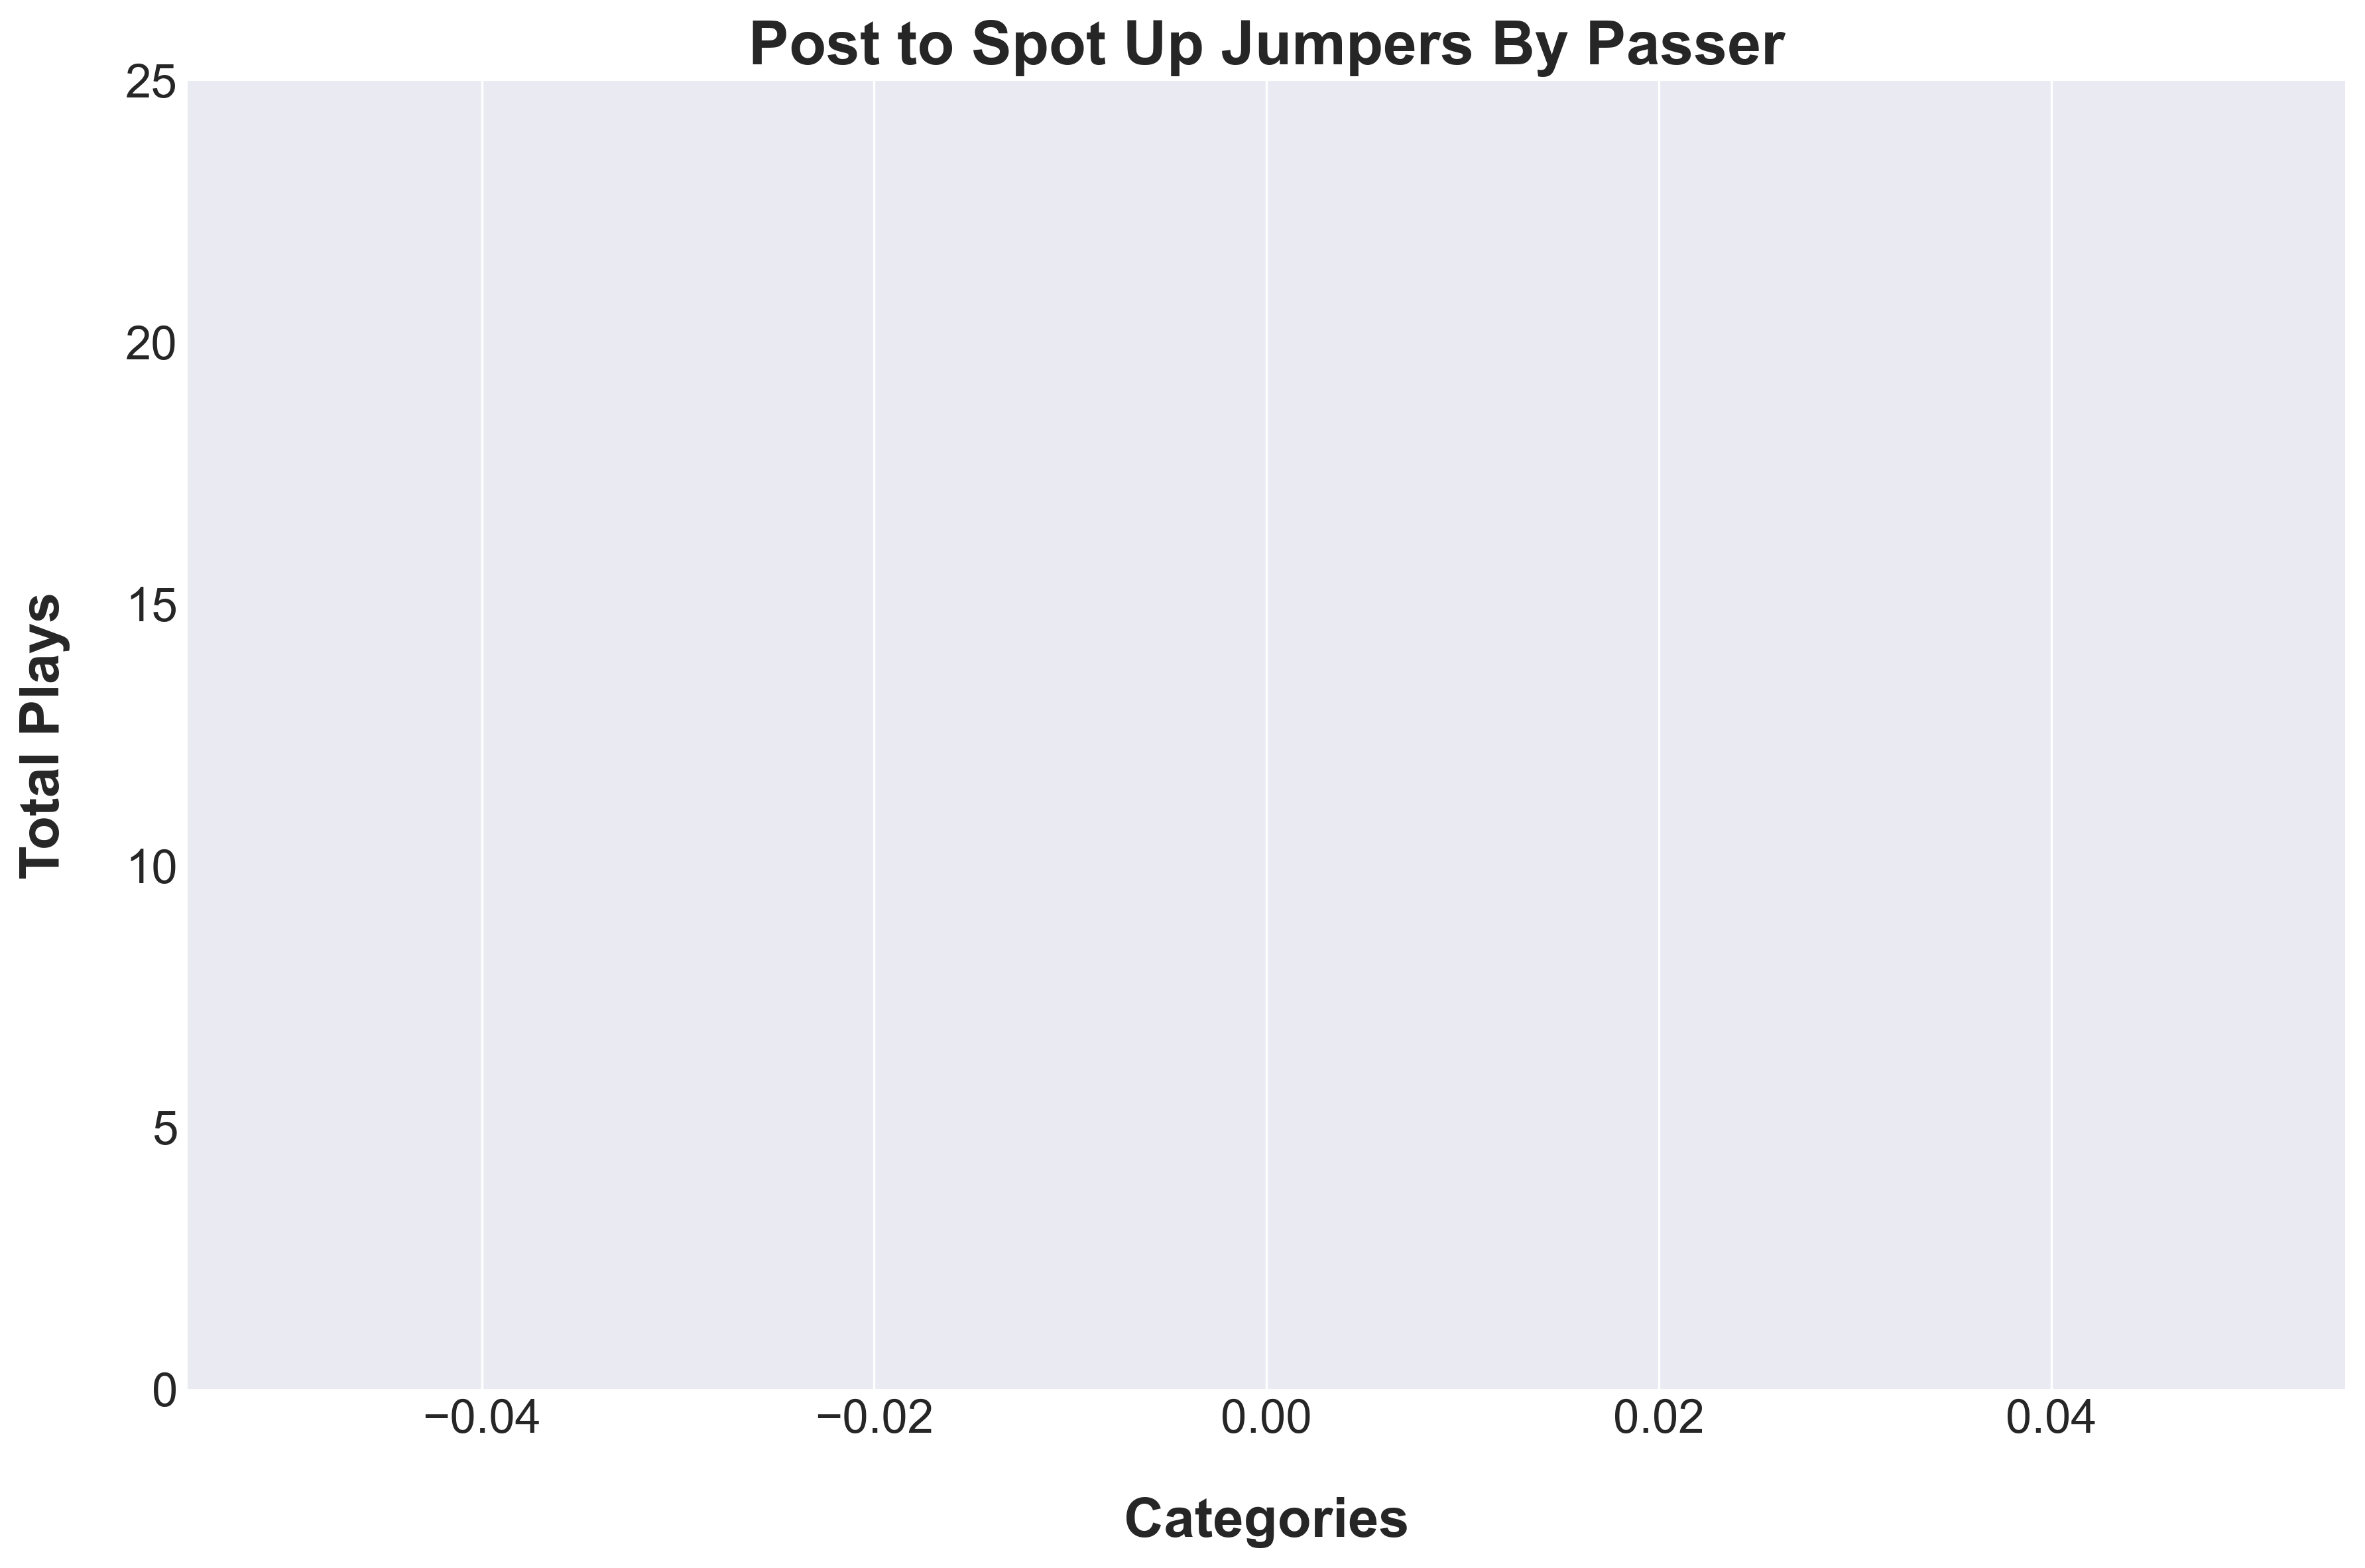
\includegraphics[width=\textwidth, height=.14\textheight]{images/SpotUp_PostShotsPlayer_Freq.png} % Adjust the width of the image to fit
    \end{minipage}
\end{table}

\vspace{-1em} % Add vertical space before the line (optional)
\vspace{-1em} % Add vertical space after the line (optional)

% Iso -> Jumpshot Stats by Passer
\begin{table}[H]
    \raisebox{3em}{ % Adjust this value to shift the tables vertically
    \begin{minipage}[t]{0.6\textwidth} % Left side (table) takes 85% of the width
        \flushleft
        \centering % Centering the title and the table
        \text{Iso - Jumpshot Stats by Passer} % Title above the table in bold
        \vskip .25em % Adds vertical space between title and table
        \scalebox{.6}{ % Scale the entire table down by half
            \renewcommand{\arraystretch}{1.4} % Adjust the number to increase or decrease row spacing
            \begin{tabular}{
            >{\centering\arraybackslash}p{3cm} 
            >{\centering\arraybackslash}p{.75cm} 
            >{\centering\arraybackslash}p{.75cm} 
            >{\centering\arraybackslash}p{.75cm} 
            >{\centering\arraybackslash}p{.75cm}
            >{\centering\arraybackslash}p{.75cm}
            >{\centering\arraybackslash}p{.75cm} 
            >{\centering\arraybackslash}p{.75cm}
            >{\centering\arraybackslash}p{.75cm}
            >{\centering\arraybackslash}p{.75cm}}% Adjust column widths
            \toprule
            {\scriptsize \textbf{Player}} &
            {\scriptsize \textbf{Plays}} &
            {\scriptsize \textbf{3PA}} &
            {\scriptsize \textbf{3PM}} &
            {\scriptsize \textbf{3P\%}} & 
            {\scriptsize \textbf{MiA}} & 
            {\scriptsize \textbf{MiM}} &
            {\scriptsize \textbf{Mi\%}} &
            {\scriptsize \textbf{TO}} &
            {\scriptsize \textbf{Foul}} \\
            \midrule
            
                
            
                
            
                
            
                
            
                
            
                
            
                
                    
                        Chase Dickens & 
                        1 & 
                        0 & 
                        0 & 
                        - & 
                        1 & 
                        0 & 
                        0.0 & 
                        0 & 
                        0 \\
                    
                
            
                
            
                
            
                
            
                
            
                
            
                
            
                
            
                
            
                
            
                
            
                
            
                
            
                
            
                
            
                
            
            \bottomrule
        \end{tabular}
        } % End of \scalebox
    \end{minipage}
    } % End of raisebox, closing the adjustment
    \hfill % This adds some flexible space between the table and the image
    \begin{minipage}[c]{0.35\textwidth} % Right side (image) takes 10% of the width
        \flushright
        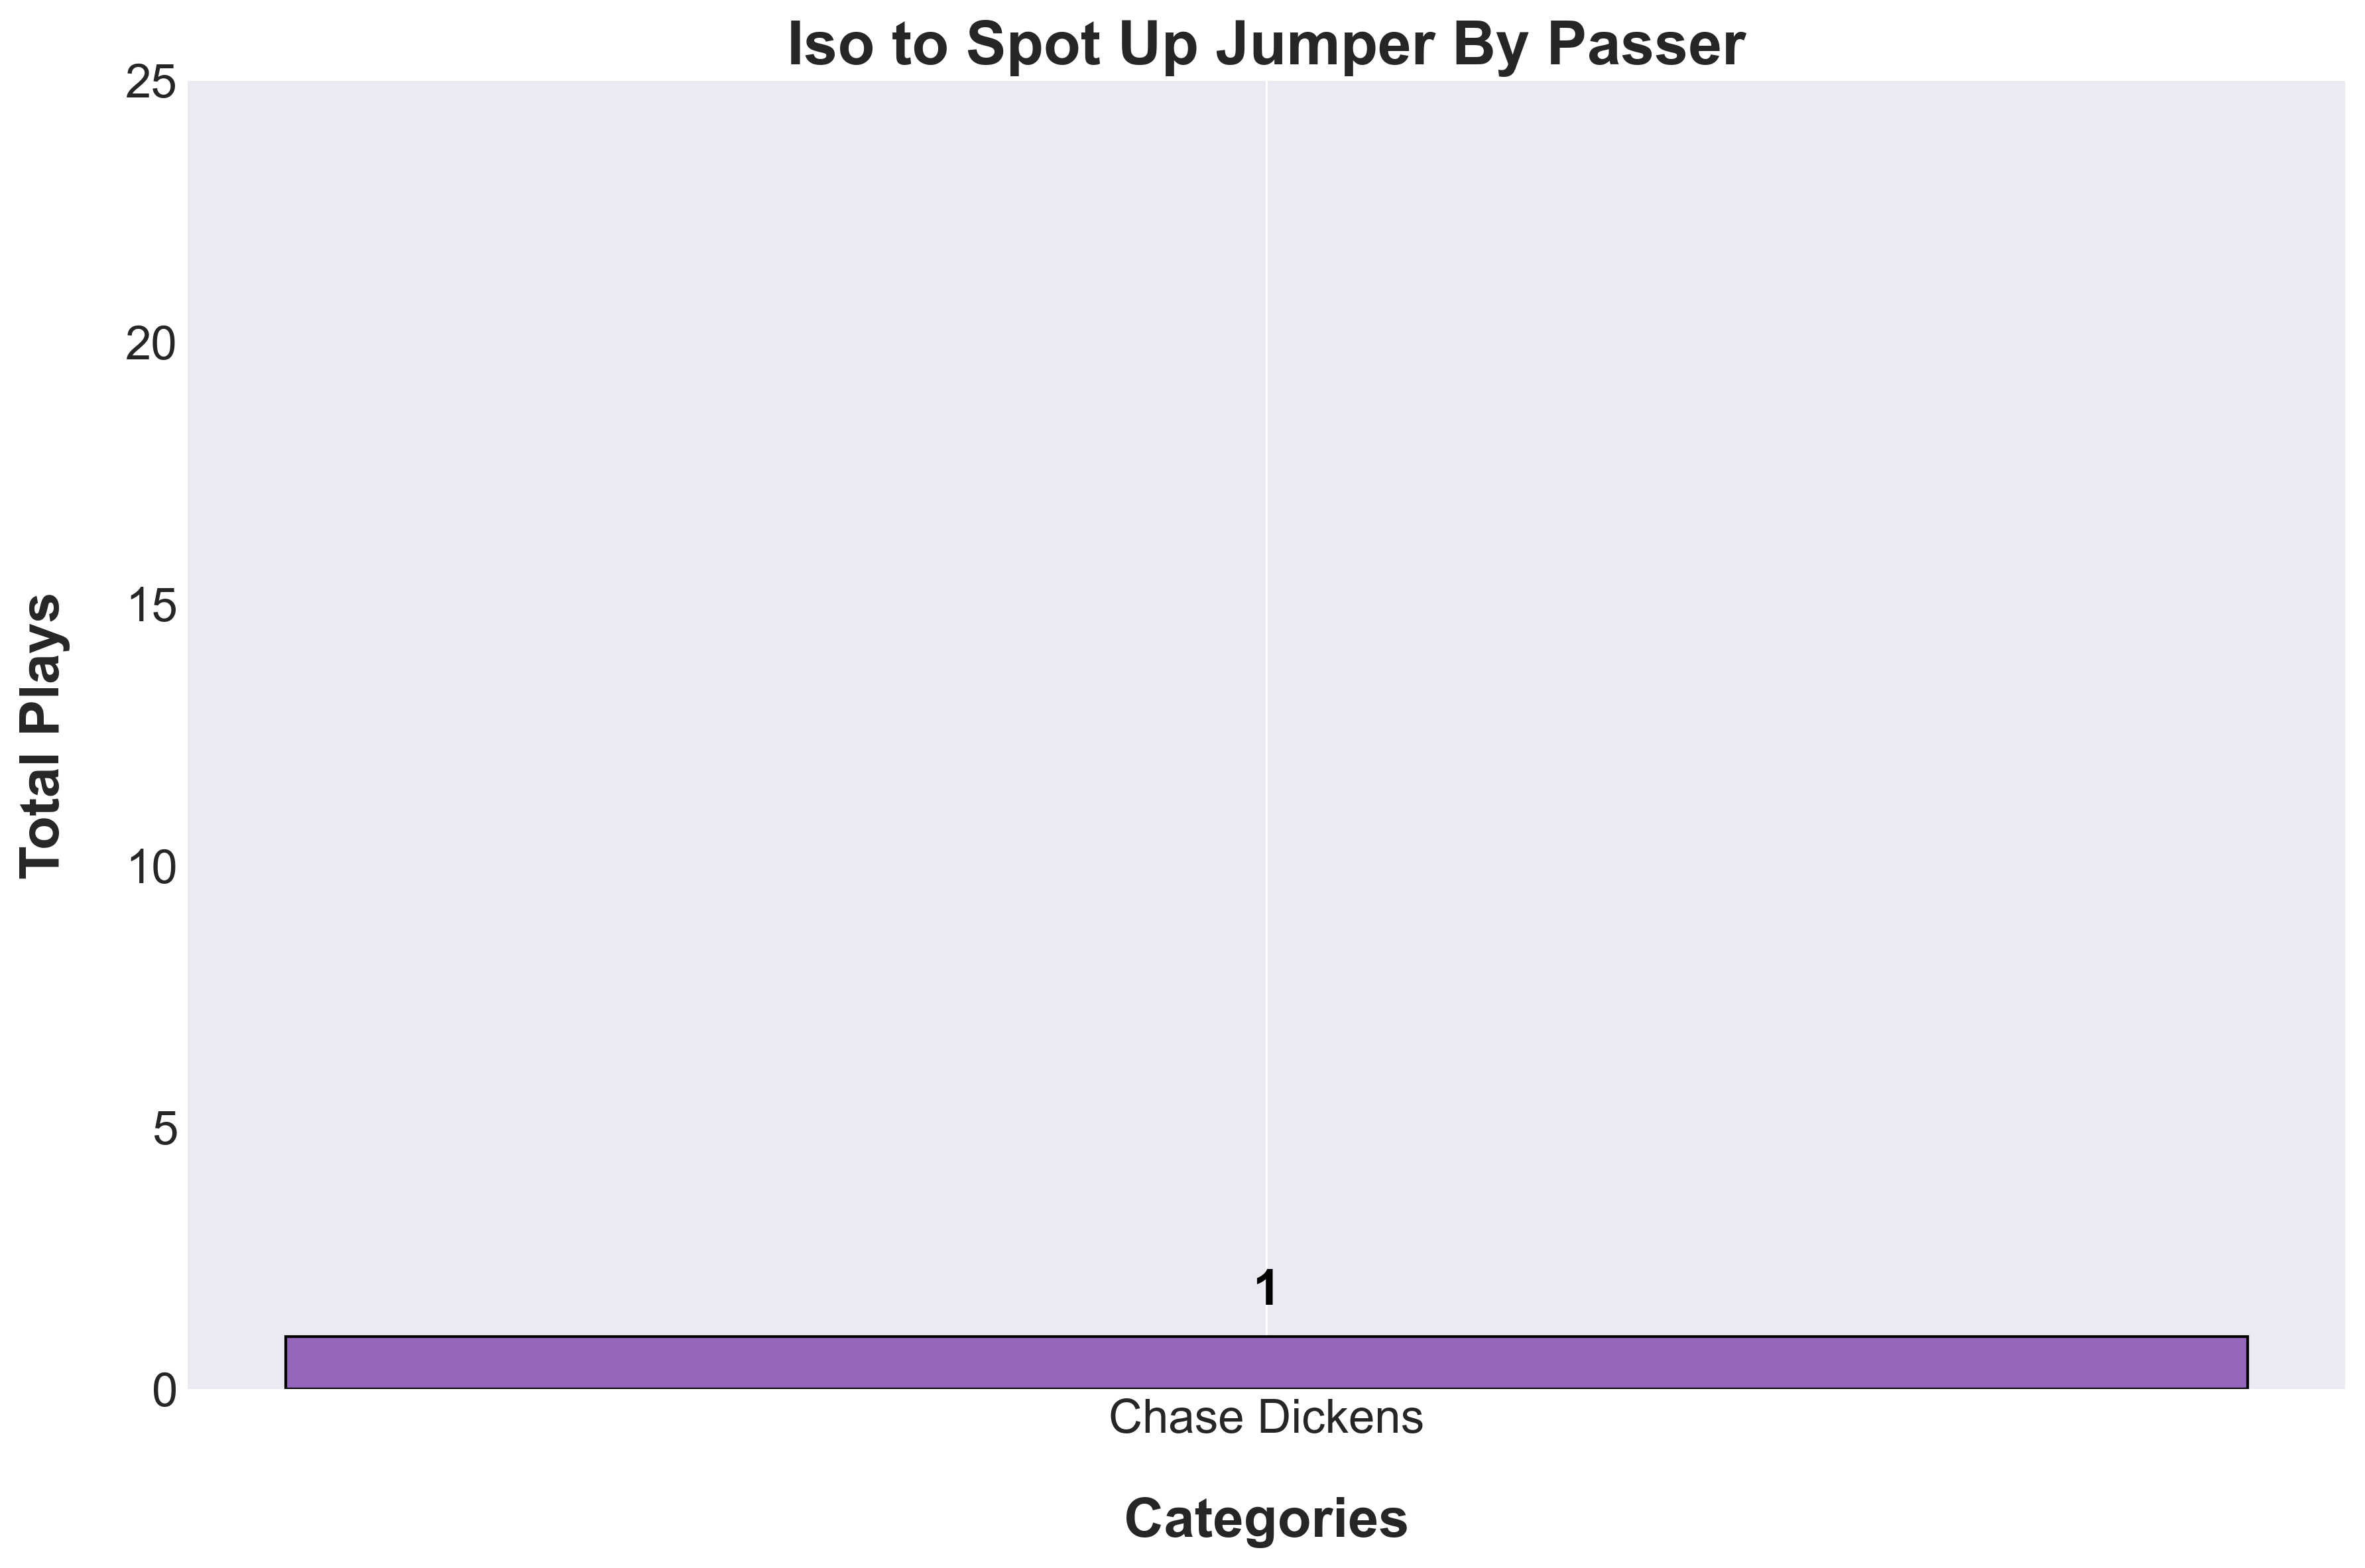
\includegraphics[width=\textwidth, height=.14\textheight]{images/SpotUp_IsoShotsPlayer_Freq.png} % Adjust the width of the image to fit
    \end{minipage}
\end{table}

\vspace{-1em} % Add vertical space before the line (optional)
\vspace{-1em} % Add vertical space after the line (optional)

% PNR -> Jumpshot Stats by Passer
\begin{table}[H]
    \raisebox{3em}{ % Adjust this value to shift the tables vertically
    \begin{minipage}[t]{0.6\textwidth} % Left side (table) takes 85% of the width
        \flushleft
        \centering % Centering the title and the table
        \text{PNR - Jumpshot Stats by Passer} % Title above the table in bold
        \vskip .25em % Adds vertical space between title and table
        \scalebox{.6}{ % Scale the entire table down by half
            \renewcommand{\arraystretch}{1.4} % Adjust the number to increase or decrease row spacing
            \begin{tabular}{
            >{\centering\arraybackslash}p{3cm} 
            >{\centering\arraybackslash}p{.75cm} 
            >{\centering\arraybackslash}p{.75cm} 
            >{\centering\arraybackslash}p{.75cm} 
            >{\centering\arraybackslash}p{.75cm} 
            >{\centering\arraybackslash}p{.75cm}
            >{\centering\arraybackslash}p{.75cm} 
            >{\centering\arraybackslash}p{.75cm}
            >{\centering\arraybackslash}p{.75cm} 
            >{\centering\arraybackslash}p{.75cm}}% Adjust column widths
            \toprule
            {\scriptsize \textbf{Player}} &
            {\scriptsize \textbf{Plays}} &
            {\scriptsize \textbf{3PA}} &
            {\scriptsize \textbf{3PM}} &
            {\scriptsize \textbf{3P\%}} & 
            {\scriptsize \textbf{MiA}} & 
            {\scriptsize \textbf{MiM}} &
            {\scriptsize \textbf{Mi\%}} &
            {\scriptsize \textbf{TO}} &
            {\scriptsize \textbf{Foul}} \\
            \midrule
            
                
            
                
            
                
            
                
            
                
            
                
            
                
            
                
            
                
            
                
            
                
                    
                        Matt Caggiano & 
                        3 & 
                        1 & 
                        1 & 
                        100.0 & 
                        2 & 
                        0 & 
                        0.0 & 
                        0 & 
                        0 \\
                    
                
            
                
            
                
            
                
            
                
            
                
            
                
            
                
            
                
            
                
            
                
            
                
            

            \bottomrule
        \end{tabular}
        } % End of \scalebox
    \end{minipage}
    } % End of raisebox, closing the adjustment
    \hfill % This adds some flexible space between the table and the image
    \begin{minipage}[c]{0.35\textwidth} % Right side (image) takes 10% of the width
        \flushright
        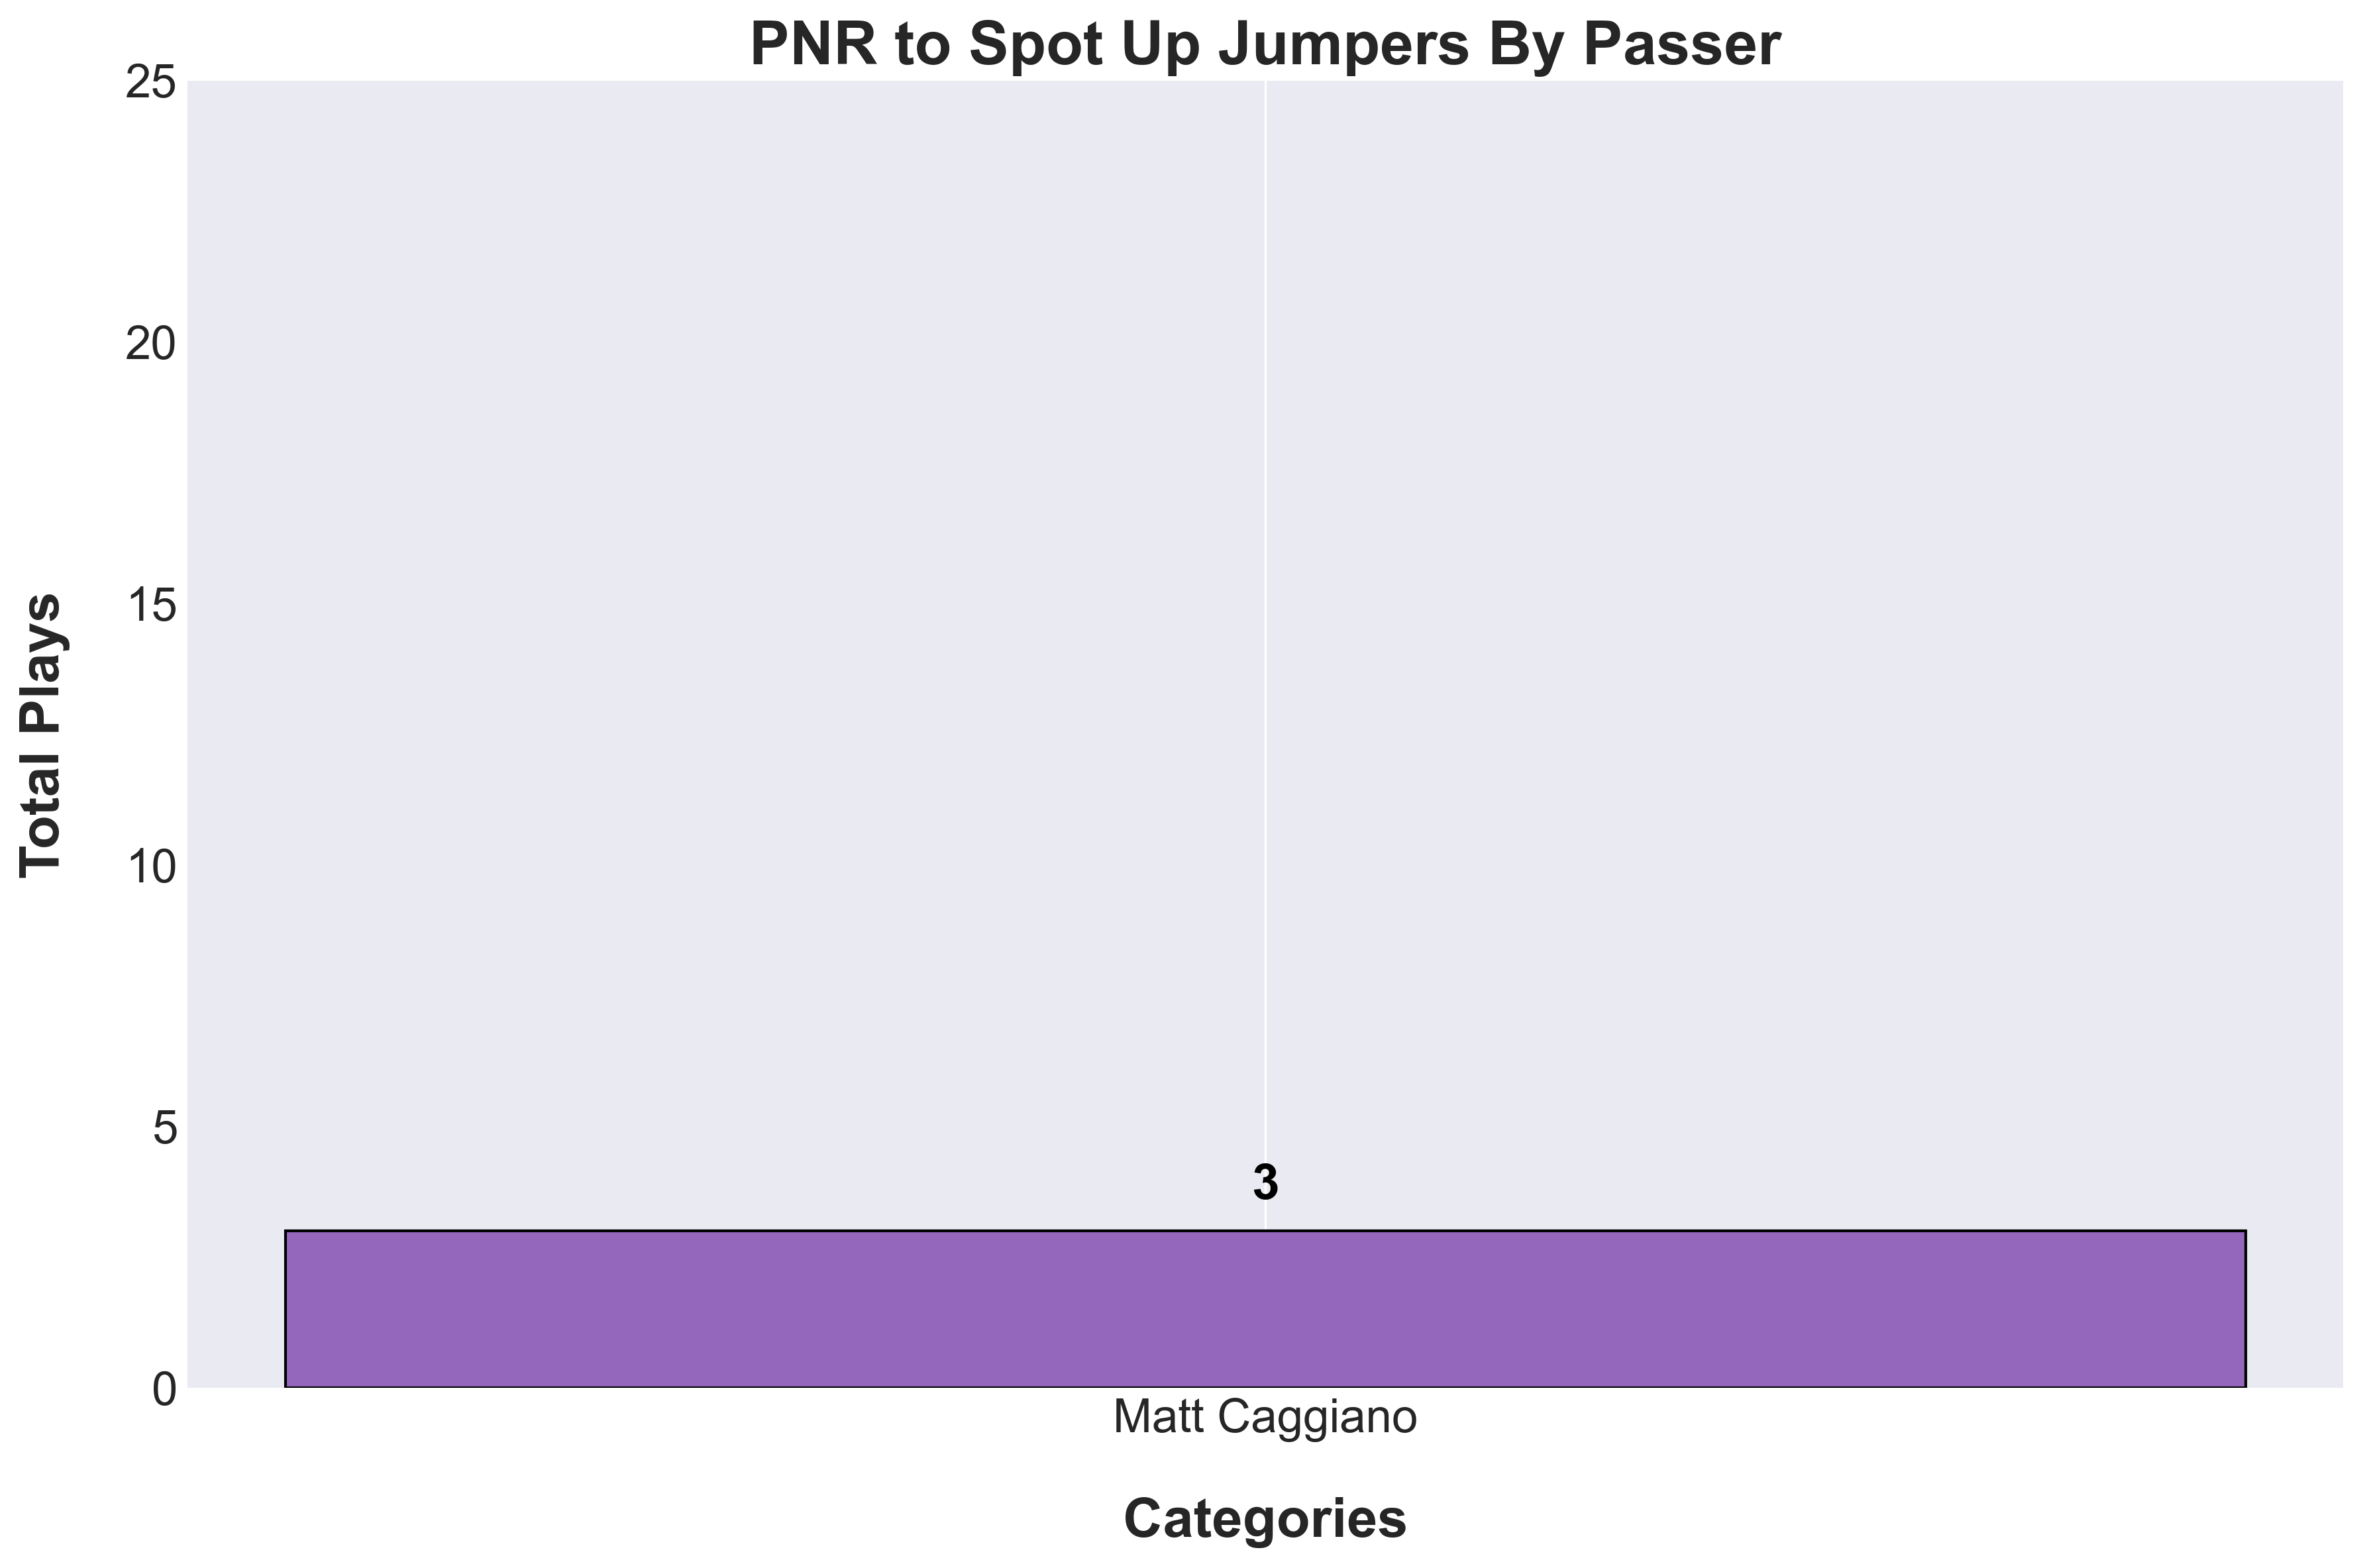
\includegraphics[width=\textwidth, height=.14\textheight]{images/SpotUp_PNRShotsPlayer_Freq.png} % Adjust the width of the image to fit
    \end{minipage}
\end{table}

\vspace{-1em} % Add vertical space before the line (optional)
\vspace{-1em} % Add vertical space after the line (optional)

% Post -> Drive Stats by Passer
\begin{table}[H]
    \raisebox{3em}{ % Adjust this value to shift the tables vertically
    \begin{minipage}[t]{0.6\textwidth} % Left side (table) takes 85% of the width
        \flushleft
        \centering % Centering the title and the table
        \text{Post - Drive Stats by Passer} % Title above the table in bold
        \vskip .25em % Adds vertical space between title and table
        \scalebox{.55}{ % Scale the entire table down by half
            \renewcommand{\arraystretch}{1.4} % Adjust the number to increase or decrease row spacing
            \begin{tabular}{
            >{\centering\arraybackslash}p{3cm} 
            >{\centering\arraybackslash}p{.75cm} 
            >{\centering\arraybackslash}p{.75cm} 
            >{\centering\arraybackslash}p{.75cm} 
            >{\centering\arraybackslash}p{.75cm}
            >{\centering\arraybackslash}p{.75cm} 
            >{\centering\arraybackslash}p{.75cm} 
            >{\centering\arraybackslash}p{.75cm} 
            >{\centering\arraybackslash}p{.75cm}
            >{\centering\arraybackslash}p{.75cm} 
            >{\centering\arraybackslash}p{.75cm}
            >{\centering\arraybackslash}p{.75cm} 
            >{\centering\arraybackslash}p{.75cm}}% Adjust column widths
            \toprule
            {\scriptsize \textbf{Player}} &
            {\scriptsize \textbf{Plays}} &
            {\scriptsize \textbf{3PA}} &
            {\scriptsize \textbf{3PM}} &
            {\scriptsize \textbf{3P\%}} & 
            {\scriptsize \textbf{2PA}} & 
            {\scriptsize \textbf{2PM}} & 
            {\scriptsize \textbf{2P\%}} & 
            {\scriptsize \textbf{MiA}} & 
            {\scriptsize \textbf{MiM}} &
            {\scriptsize \textbf{Mi\%}} &
            {\scriptsize \textbf{TO}} &
            {\scriptsize \textbf{Foul}} \\
            \midrule
            
                
            
                
            
                
            
                
            
                
            
                
            
                
            
                
            
                
            
                
            
                
            
                
            
                
                    
                
            
                
            
                
            
                
            
                
            
                
            
                
            
                
            
                
            
                
            

            \bottomrule
        \end{tabular}
        } % End of \scalebox
    \end{minipage}
    } % End of raisebox, closing the adjustment
    \hfill % This adds some flexible space between the table and the image
    \begin{minipage}[c]{0.35\textwidth} % Right side (image) takes 10% of the width
        \flushright
        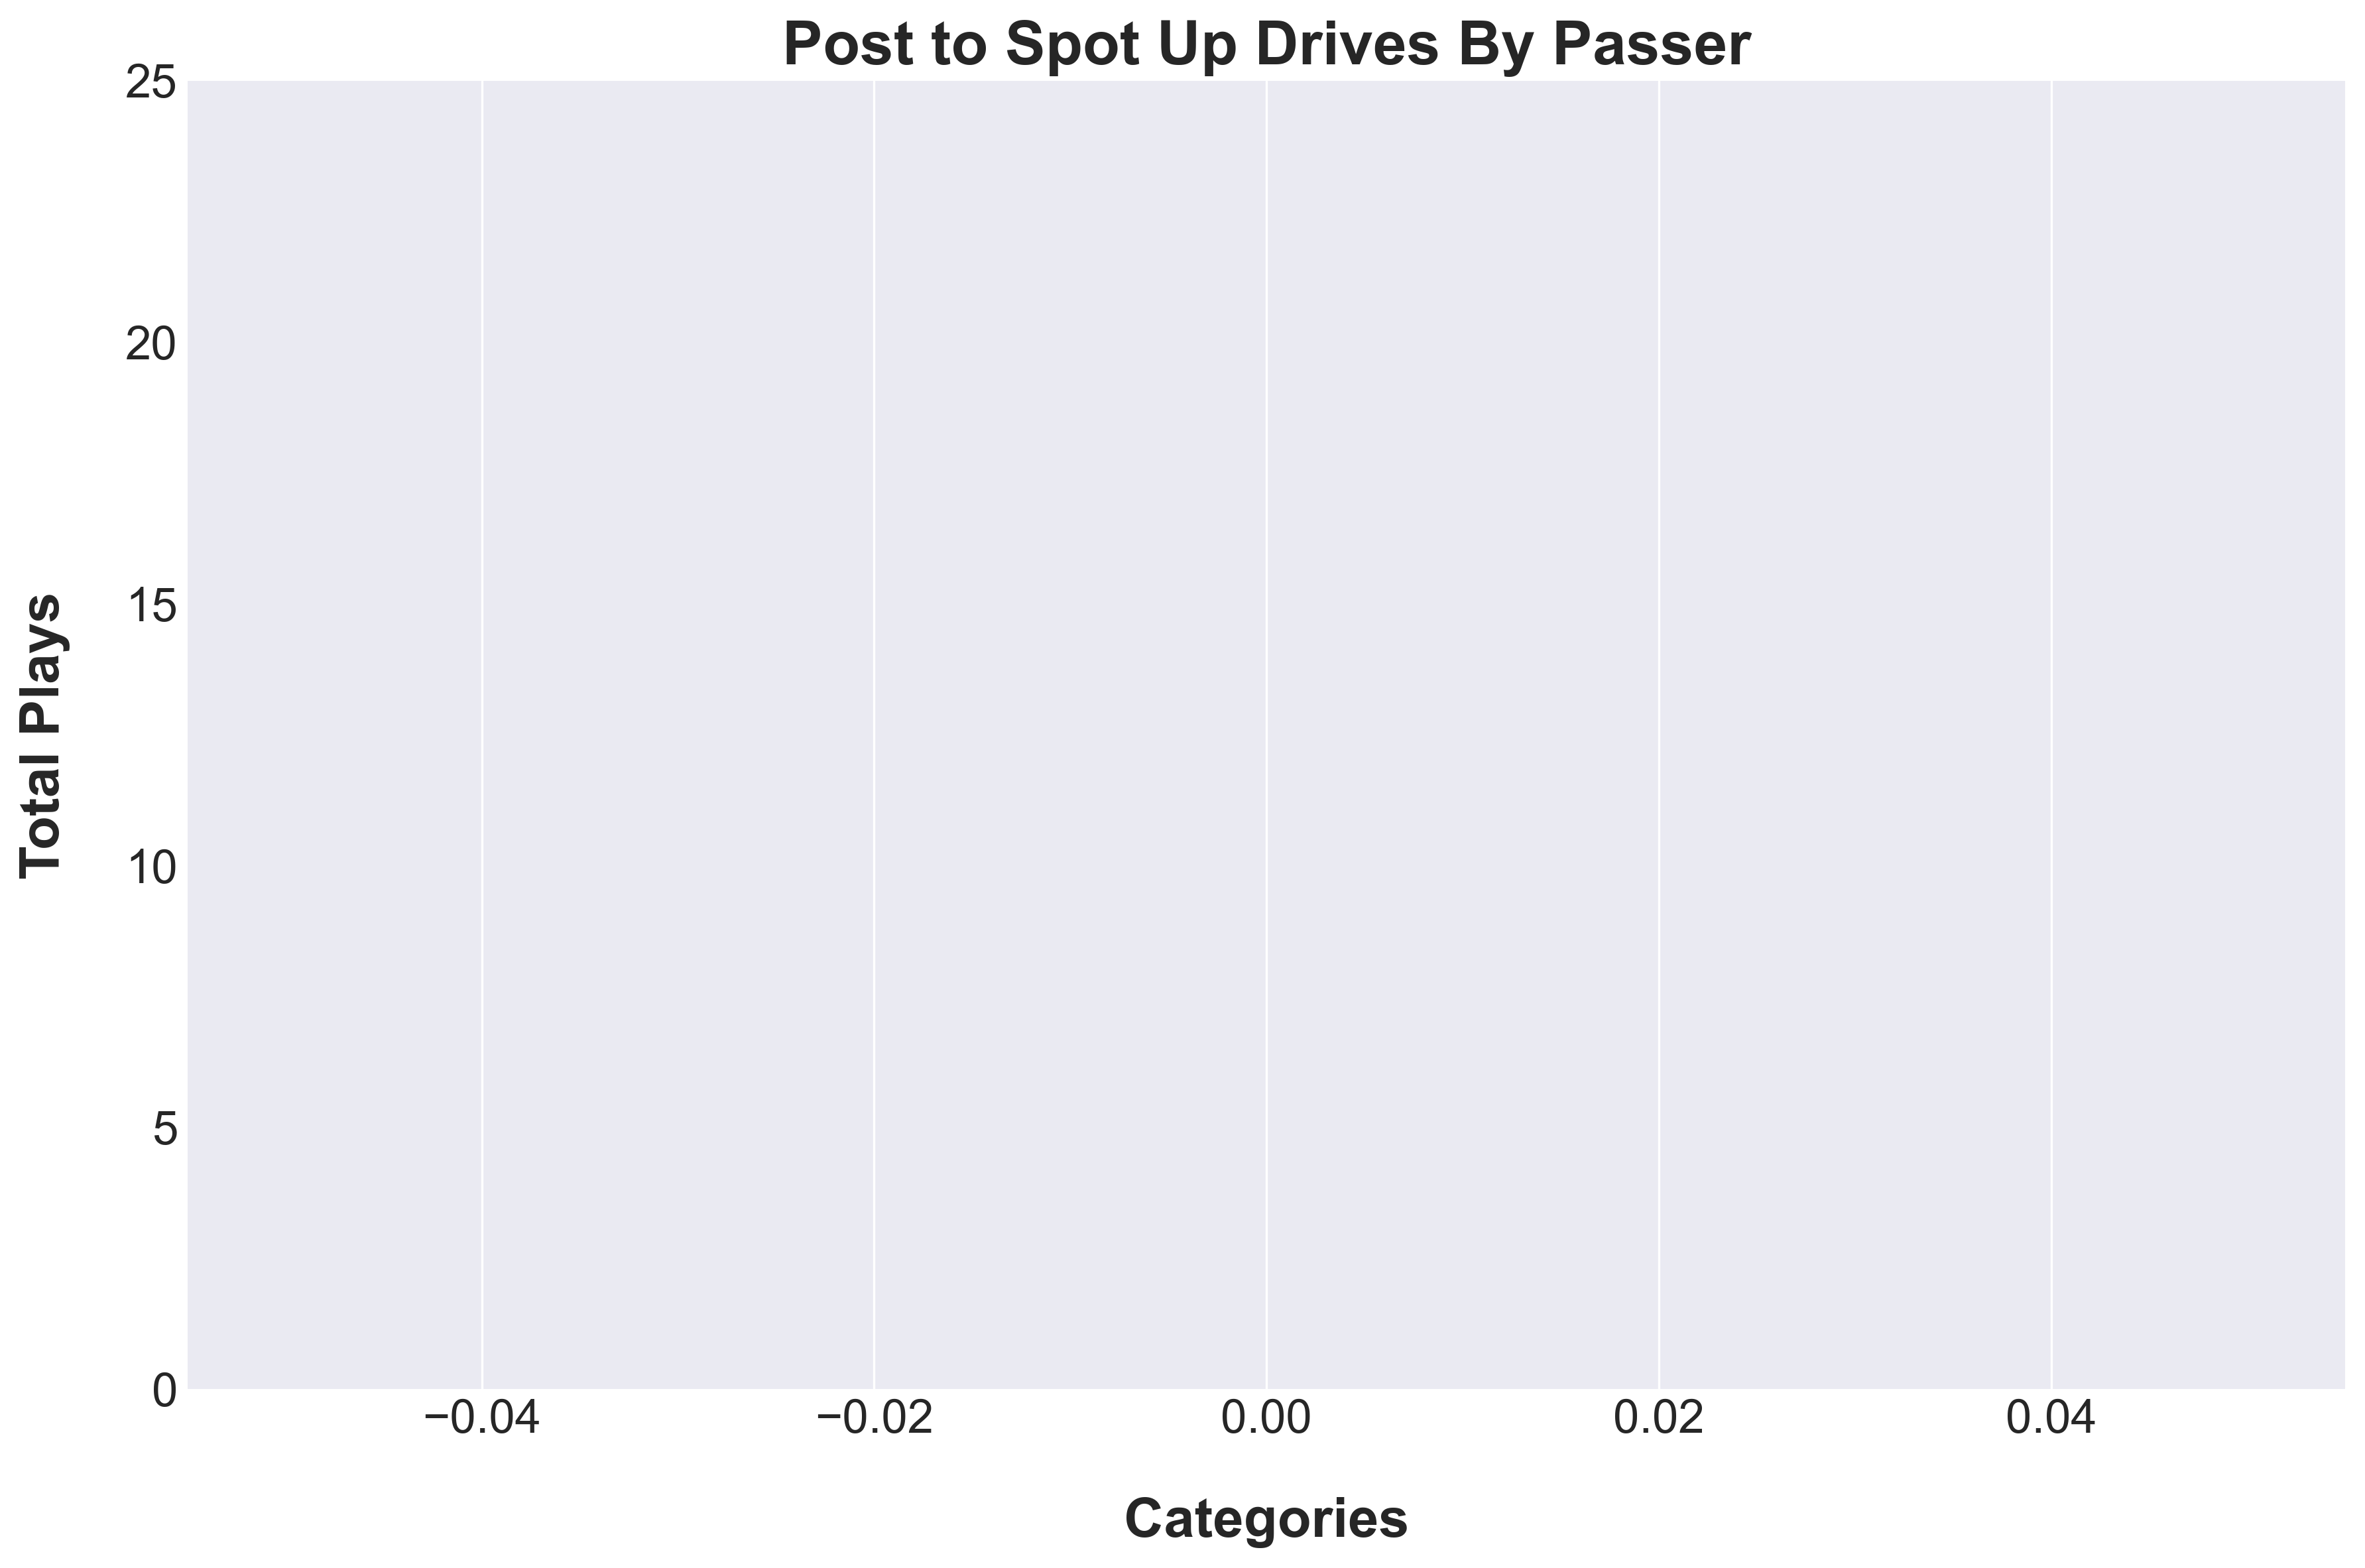
\includegraphics[width=\textwidth, height=.14\textheight]{images/SpotUp_PostDrivesPlayer_Freq.png} % Adjust the width of the image to fit
    \end{minipage}
\end{table}

\vspace{-1em} % Add vertical space before the line (optional)
\vspace{-1em} % Add vertical space after the line (optional)

% Iso -> Drive Stats by Passer
\begin{table}[H]
    \raisebox{3em}{ % Adjust this value to shift the tables vertically
    \begin{minipage}[t]{0.6\textwidth} % Left side (table) takes 85% of the width
        \flushleft
        \centering % Centering the title and the table
        \text{Iso - Drive Stats by Passer} % Title above the table in bold
        \vskip .25em % Adds vertical space between title and table
        \scalebox{.55}{ % Scale the entire table down by half
            \renewcommand{\arraystretch}{1.4} % Adjust the number to increase or decrease row spacing
            \begin{tabular}{
            >{\centering\arraybackslash}p{3cm} 
            >{\centering\arraybackslash}p{.75cm} 
            >{\centering\arraybackslash}p{.75cm} 
            >{\centering\arraybackslash}p{.75cm} 
            >{\centering\arraybackslash}p{.75cm}
            >{\centering\arraybackslash}p{.75cm} 
            >{\centering\arraybackslash}p{.75cm} 
            >{\centering\arraybackslash}p{.75cm} 
            >{\centering\arraybackslash}p{.75cm}
            >{\centering\arraybackslash}p{.75cm} 
            >{\centering\arraybackslash}p{.75cm}
            >{\centering\arraybackslash}p{.75cm} 
            >{\centering\arraybackslash}p{.75cm}}% Adjust column widths
            \toprule
            {\scriptsize \textbf{Player}} &
            {\scriptsize \textbf{Plays}} &
            {\scriptsize \textbf{3PA}} &
            {\scriptsize \textbf{3PM}} &
            {\scriptsize \textbf{3P\%}} & 
            {\scriptsize \textbf{2PA}} & 
            {\scriptsize \textbf{2PM}} & 
            {\scriptsize \textbf{2P\%}} & 
            {\scriptsize \textbf{MiA}} & 
            {\scriptsize \textbf{MiM}} &
            {\scriptsize \textbf{Mi\%}} &
            {\scriptsize \textbf{TO}} &
            {\scriptsize \textbf{Foul}} \\
            \midrule
            
                
            
                
            
                
            
                
            
                
                    
                
            
                
            
                
            
                
            
                
            
                
            
                
            
                
            
                
            
                
            
                
            
                
            
                
            
                
            
                
            
                
            
                
            
                
            

            \bottomrule
        \end{tabular}
        } % End of \scalebox
    \end{minipage}
    } % End of raisebox, closing the adjustment
    \hfill % This adds some flexible space between the table and the image
    \begin{minipage}[c]{0.35\textwidth} % Right side (image) takes 10% of the width
        \flushright
        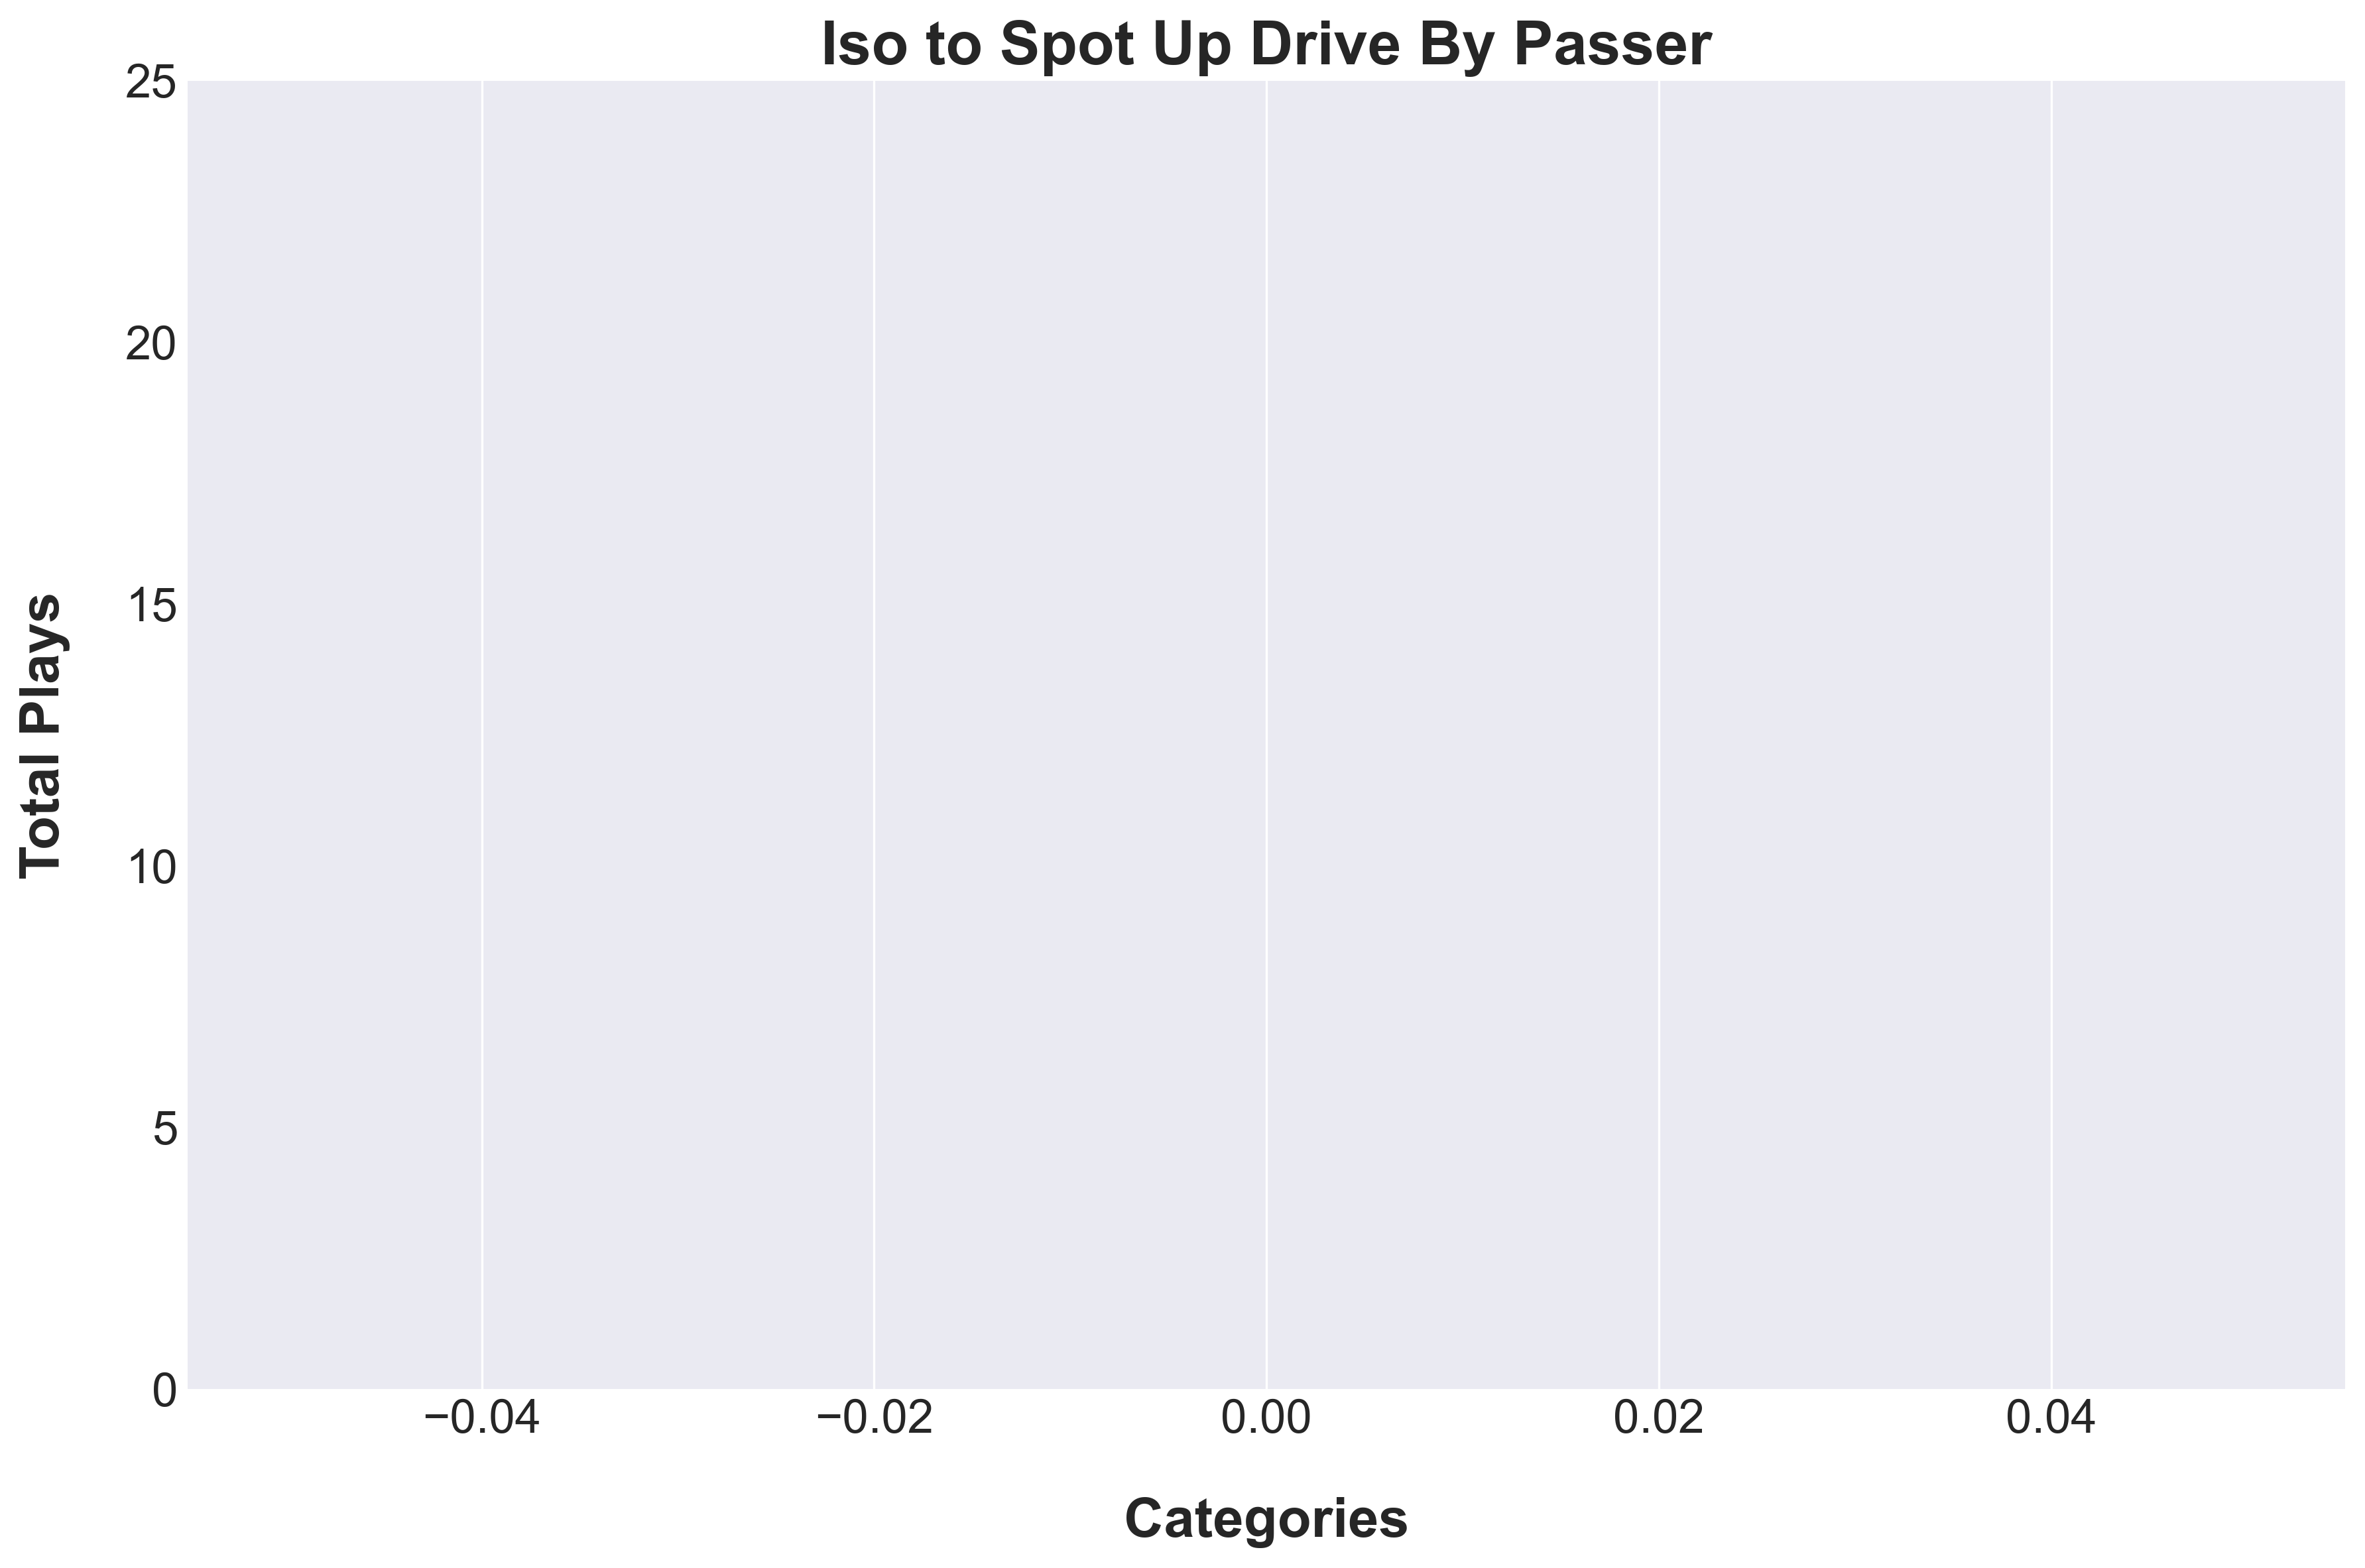
\includegraphics[width=\textwidth, height=.14\textheight]{images/SpotUp_IsoDrivesPlayer_Freq.png} % Adjust the width of the image to fit
    \end{minipage}
\end{table}

\vspace{-1em} % Add vertical space before the line (optional)
\vspace{-1em} % Add vertical space after the line (optional)

% PNR -> Drive Stats by Passer
\begin{table}[H]
    \raisebox{3em}{ % Adjust this value to shift the tables vertically
    \begin{minipage}[t]{0.6\textwidth} % Left side (table) takes 85% of the width
        \flushleft
        \centering % Centering the title and the table
        \text{PNR - Drive Stats by Passer} % Title above the table in bold
        \vskip .25em % Adds vertical space between title and table
        \scalebox{.55}{ % Scale the entire table down by half
            \renewcommand{\arraystretch}{1.4} % Adjust the number to increase or decrease row spacing
            \begin{tabular}{
            >{\centering\arraybackslash}p{3cm} 
            >{\centering\arraybackslash}p{.75cm} 
            >{\centering\arraybackslash}p{.75cm} 
            >{\centering\arraybackslash}p{.75cm} 
            >{\centering\arraybackslash}p{.75cm}
            >{\centering\arraybackslash}p{.75cm} 
            >{\centering\arraybackslash}p{.75cm} 
            >{\centering\arraybackslash}p{.75cm} 
            >{\centering\arraybackslash}p{.75cm}
            >{\centering\arraybackslash}p{.75cm} 
            >{\centering\arraybackslash}p{.75cm}
            >{\centering\arraybackslash}p{.75cm}
            >{\centering\arraybackslash}p{.75cm} 
            >{\centering\arraybackslash}p{.75cm}}% Adjust column widths
            \toprule
            {\scriptsize \textbf{Player}} &
            {\scriptsize \textbf{Plays}} &
            {\scriptsize \textbf{3PA}} &
            {\scriptsize \textbf{3PM}} &
            {\scriptsize \textbf{3P\%}} & 
            {\scriptsize \textbf{2PA}} & 
            {\scriptsize \textbf{2PM}} & 
            {\scriptsize \textbf{2P\%}} & 
            {\scriptsize \textbf{MiA}} & 
            {\scriptsize \textbf{MiM}} &
            {\scriptsize \textbf{Mi\%}} &
            {\scriptsize \textbf{TO}} &
            {\scriptsize \textbf{Foul}} \\
            \midrule
            
                
            
                
            
                
            
                
            
                
            
                
            
                
            
                
            
                
                    
                        Keegan Ocorr & 
                        1 & 
                        0 & 
                        0 & 
                        - & 
                        1 & 
                        0 & 
                        0.0 & 
                        1 & 
                        0 & 
                        0.0 & 
                        0 & 
                        0 \\
                    
                
            
                
            
                
            
                
            
                
            
                
            
                
            
                
            
                
            
                
            
                
            
                
            
                
            
                
            

            \bottomrule
        \end{tabular}
        } % End of \scalebox
    \end{minipage}
    } % End of raisebox, closing the adjustment
    \hfill % This adds some flexible space between the table and the image
    \begin{minipage}[c]{0.35\textwidth} % Right side (image) takes 10% of the width
        \flushright
        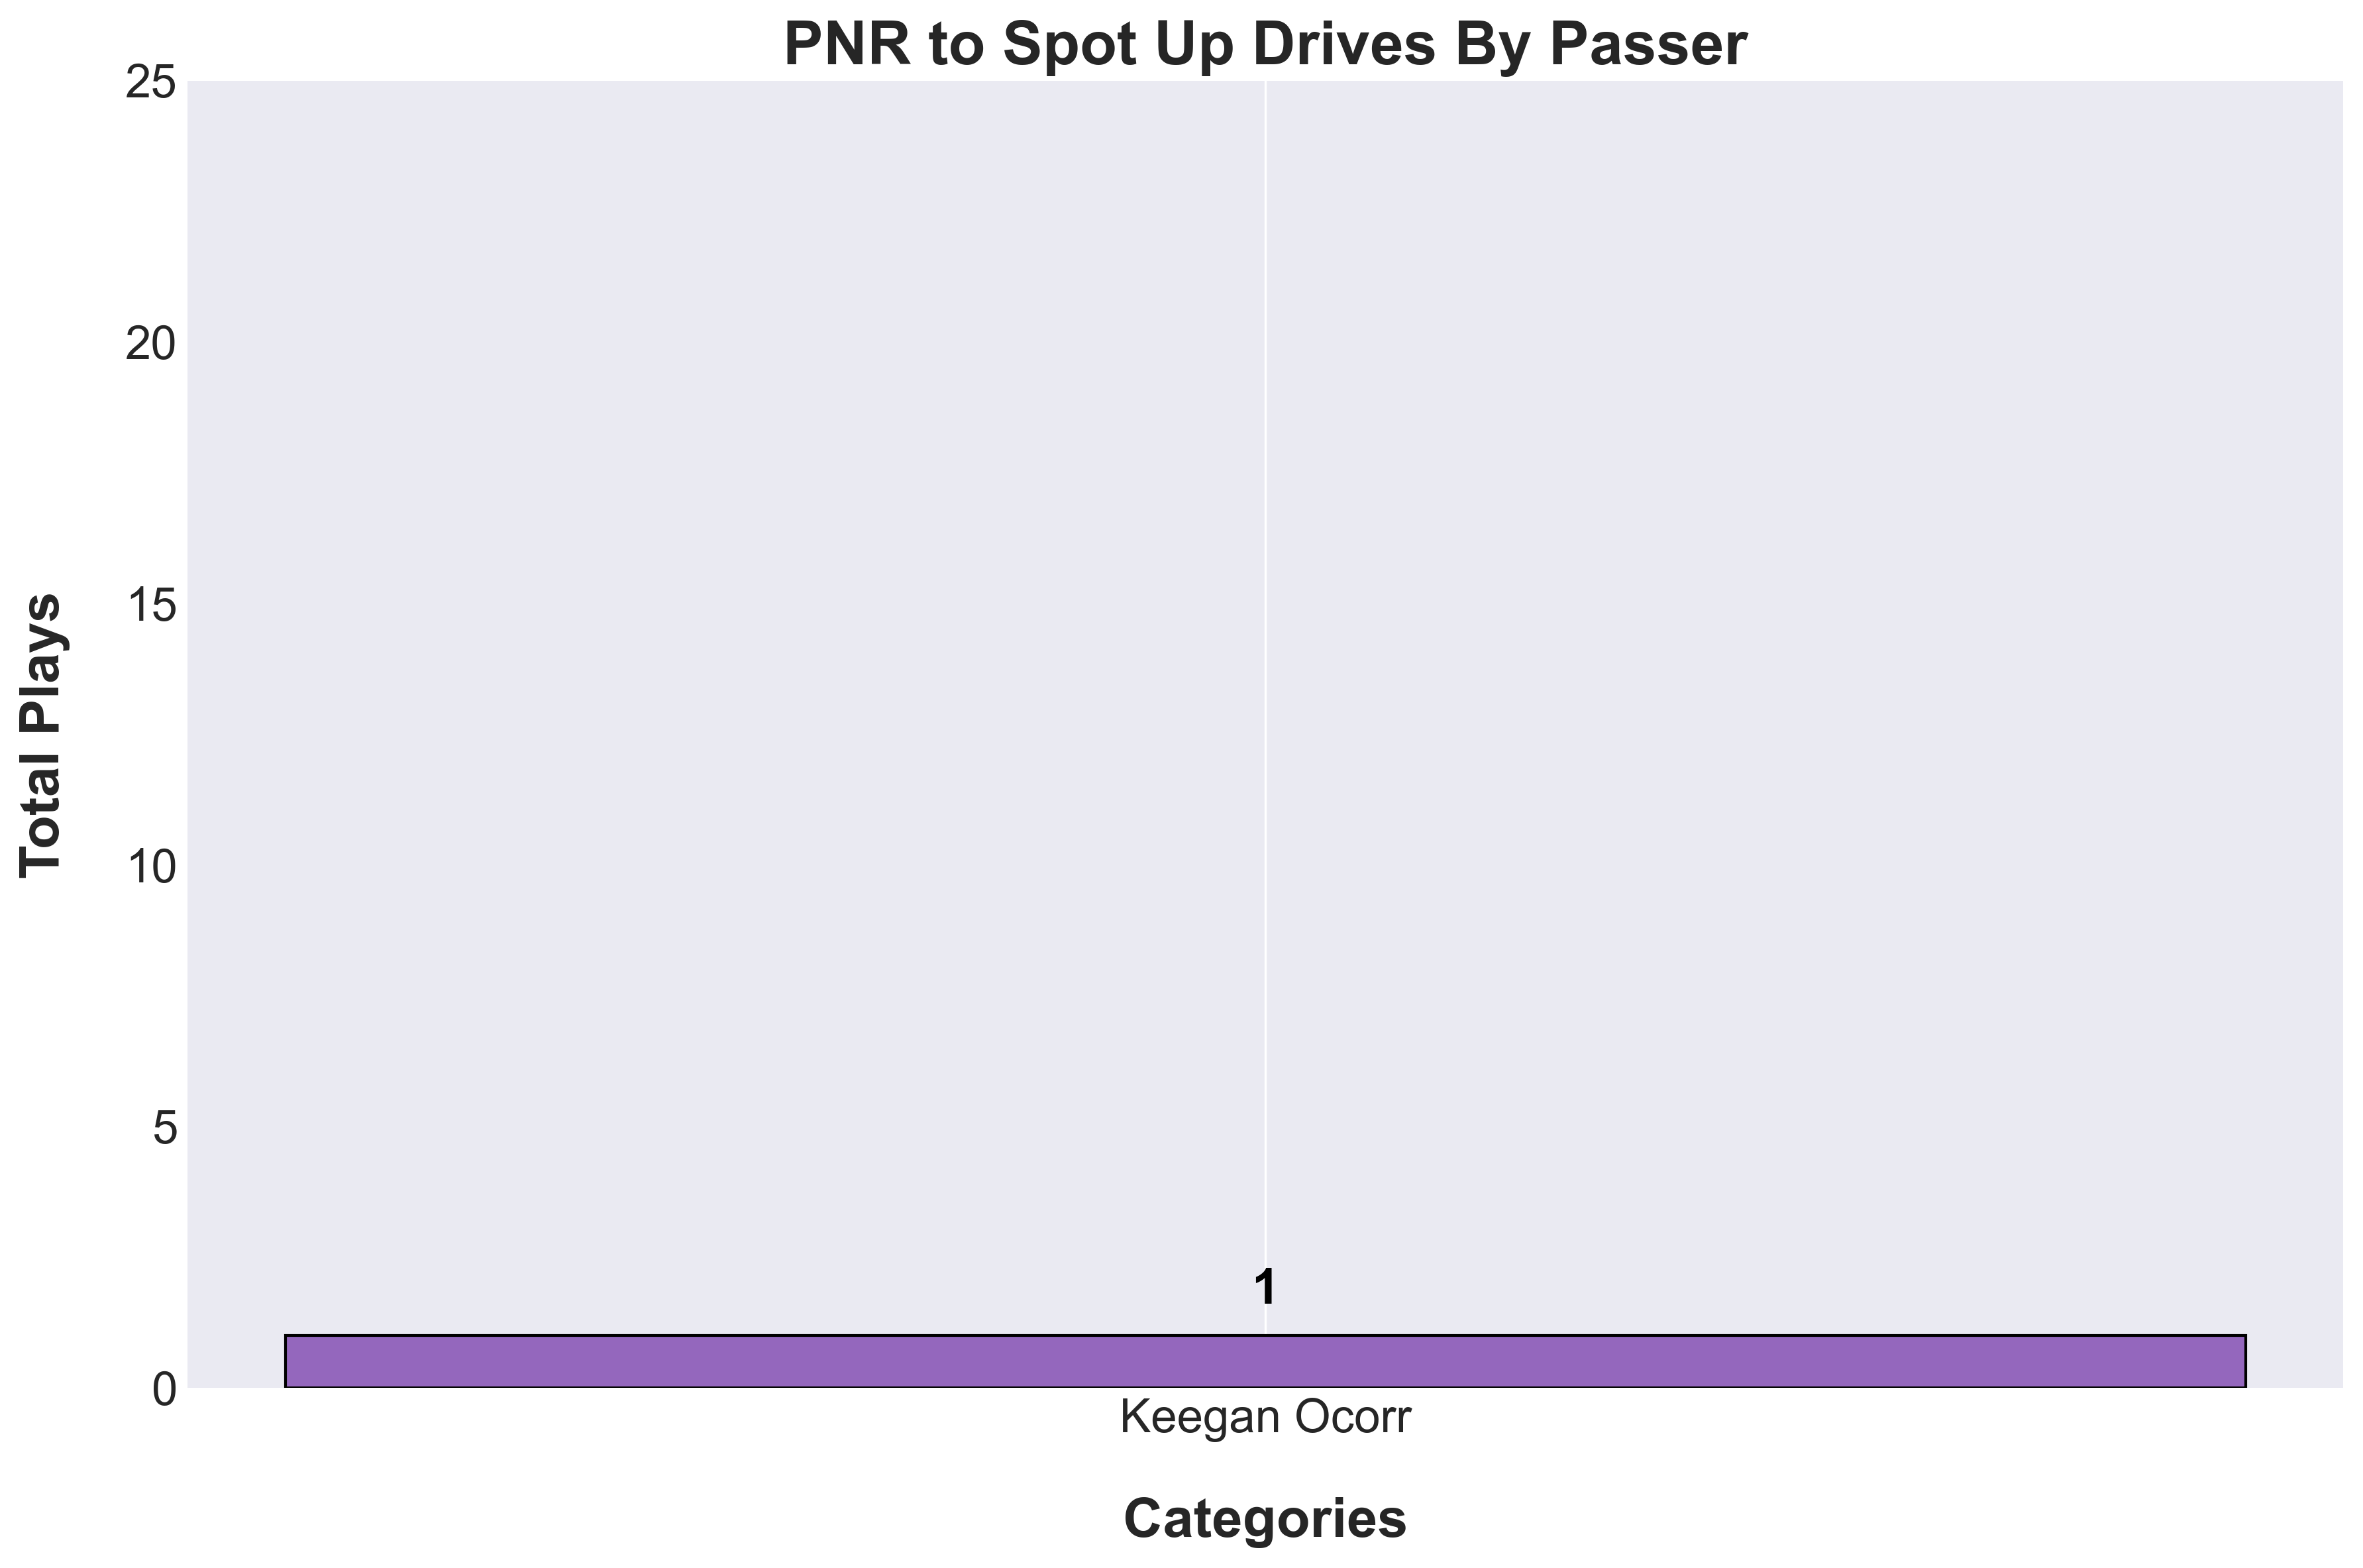
\includegraphics[width=\textwidth, height=.14\textheight]{images/SpotUp_PnrDrivesPlayer_Freq.png} % Adjust the width of the image to fit
    \end{minipage}
\end{table}

\vspace{-1em} % Add vertical space before the line (optional)
\hrule height 1pt width 1\textwidth % Adjust height and width
\vspace{1em} % Add vertical space after the line (optional)





% ----------------------
% Iso Visuals and Insights Section
% ----------------------
\subsection{Iso}

\vspace{1em} % Add vertical space after the line (optional)
\hrule height 1pt width 1\textwidth % Adjust height and width
\vspace{1em} % Add vertical space after the line (optional)

\subsubsection{General Iso Stats}
% All Cutter Statistics Table w/ room for insights
\begin{table}[H]
    \centering
    \begin{minipage}[t]{0.6\textwidth} % Left side (table) takes 85% of the width
        %\flushright
        \centering % Centering the title and the table
        \text{Total Iso Statistics} % Title above the table in bold
        \vskip .25em % Adds vertical space between title and table
        \scalebox{.85}{ % Scale the entire table down by half
            \scriptsize % Reduce the font size
            \begin{tabular}{
            >{\centering\arraybackslash}p{.75cm} 
            >{\centering\arraybackslash}p{.5cm} 
            >{\centering\arraybackslash}p{.5cm} 
            >{\centering\arraybackslash}p{.5cm}
            >{\centering\arraybackslash}p{.5cm} 
            >{\centering\arraybackslash}p{.5cm} 
            >{\centering\arraybackslash}p{.5cm} 
            >{\centering\arraybackslash}p{.5cm}
            >{\centering\arraybackslash}p{.5cm} 
            >{\centering\arraybackslash}p{.5cm}
            >{\centering\arraybackslash}p{.5cm} 
            >{\centering\arraybackslash}p{.5cm}}% Adjust column widths
            \toprule
            \textbf{Plays} &
            \textbf{3PA} &
            \textbf{3PM} &
            \textbf{3P\%} & 
            \textbf{2PA} & 
            \textbf{2PM} & 
            \textbf{2P\%} & 
            \textbf{MiA} & 
            \textbf{MiM} &
            \textbf{Mi\%} &
            \textbf{TO} &
            \textbf{Foul} \\
            \midrule
            
                
            
                
            
                
            
                
            
                
            
                
                    23 & 0 & 0 &
                    - & 
                    18 & 7 &
                    38.89 &
                    9 & 5 &
                    55.56 &
                    3 & 2 \\
                
            
                
            
                
            
                
            
                
            


            \bottomrule
            \end{tabular}
        }
    \end{minipage}
\end{table}

\vspace{0em} % Add vertical space before the line (optional)
%\hrule height 1pt width 1\textwidth % Adjust height and width
\vspace{-1em} % Add vertical space after the line (optional)

% Iso Stats for Top vs Right vs Left 
\begin{table}[H]
    \raisebox{3em}{ % Adjust this value to shift the tables vertically
    \begin{minipage}[t]{0.6\textwidth} % Left side (table) takes 85% of the width
        \flushleft
        \centering % Centering the title and the table
        \text{Iso Direction/Location Statistics} % Title above the table in bold
        \vskip .25em % Adds vertical space between title and table
        \scalebox{.6}{ % Scale the entire table down by half
            \renewcommand{\arraystretch}{1.4} % Adjust the number to increase or decrease row spacing
            \begin{tabular}{
            >{\centering\arraybackslash}p{1.75cm} 
            >{\centering\arraybackslash}p{.75cm} 
            >{\centering\arraybackslash}p{.75cm} 
            >{\centering\arraybackslash}p{.75cm} 
            >{\centering\arraybackslash}p{.75cm}
            >{\centering\arraybackslash}p{.75cm} 
            >{\centering\arraybackslash}p{.75cm} 
            >{\centering\arraybackslash}p{.75cm} 
            >{\centering\arraybackslash}p{.75cm}
            >{\centering\arraybackslash}p{.75cm} 
            >{\centering\arraybackslash}p{.75cm}
            >{\centering\arraybackslash}p{.75cm} 
            >{\centering\arraybackslash}p{.75cm}}% Adjust column widths
            \toprule
            {\scriptsize \textbf{PlayType}} &
            {\scriptsize \textbf{Plays}} &
            {\scriptsize \textbf{3PA}} &
            {\scriptsize \textbf{3PM}} &
            {\scriptsize \textbf{3P\%}} & 
            {\scriptsize \textbf{2PA}} & 
            {\scriptsize \textbf{2PM}} & 
            {\scriptsize \textbf{2P\%}} & 
            {\scriptsize \textbf{MiA}} & 
            {\scriptsize \textbf{MiM}} &
            {\scriptsize \textbf{Mi\%}} &
            {\scriptsize \textbf{TO}} &
            {\scriptsize \textbf{Foul}} \\
            \midrule
            
                
            
                
            
                
            
                
            
                
            
                
            
                
            
                
            
                
                    Right & 1 & 0 & 0 &
                    - & 
                    1 & 0 &
                    0.0 &
                    1 & 0 &
                    0.0 &
                    0 & 0 \\
                
            
                
                    Top & 22 & 0 & 0 &
                    - & 
                    17 & 7 &
                    41.18 &
                    8 & 5 &
                    62.5 &
                    3 & 2 \\
                
            


            \bottomrule
        \end{tabular}
        } % End of \scalebox
    \end{minipage}
    } % End of raisebox, closing the adjustment
    \hfill % This adds some flexible space between the table and the image
    \begin{minipage}[c]{0.35\textwidth} % Right side (image) takes 10% of the width
        \flushright
        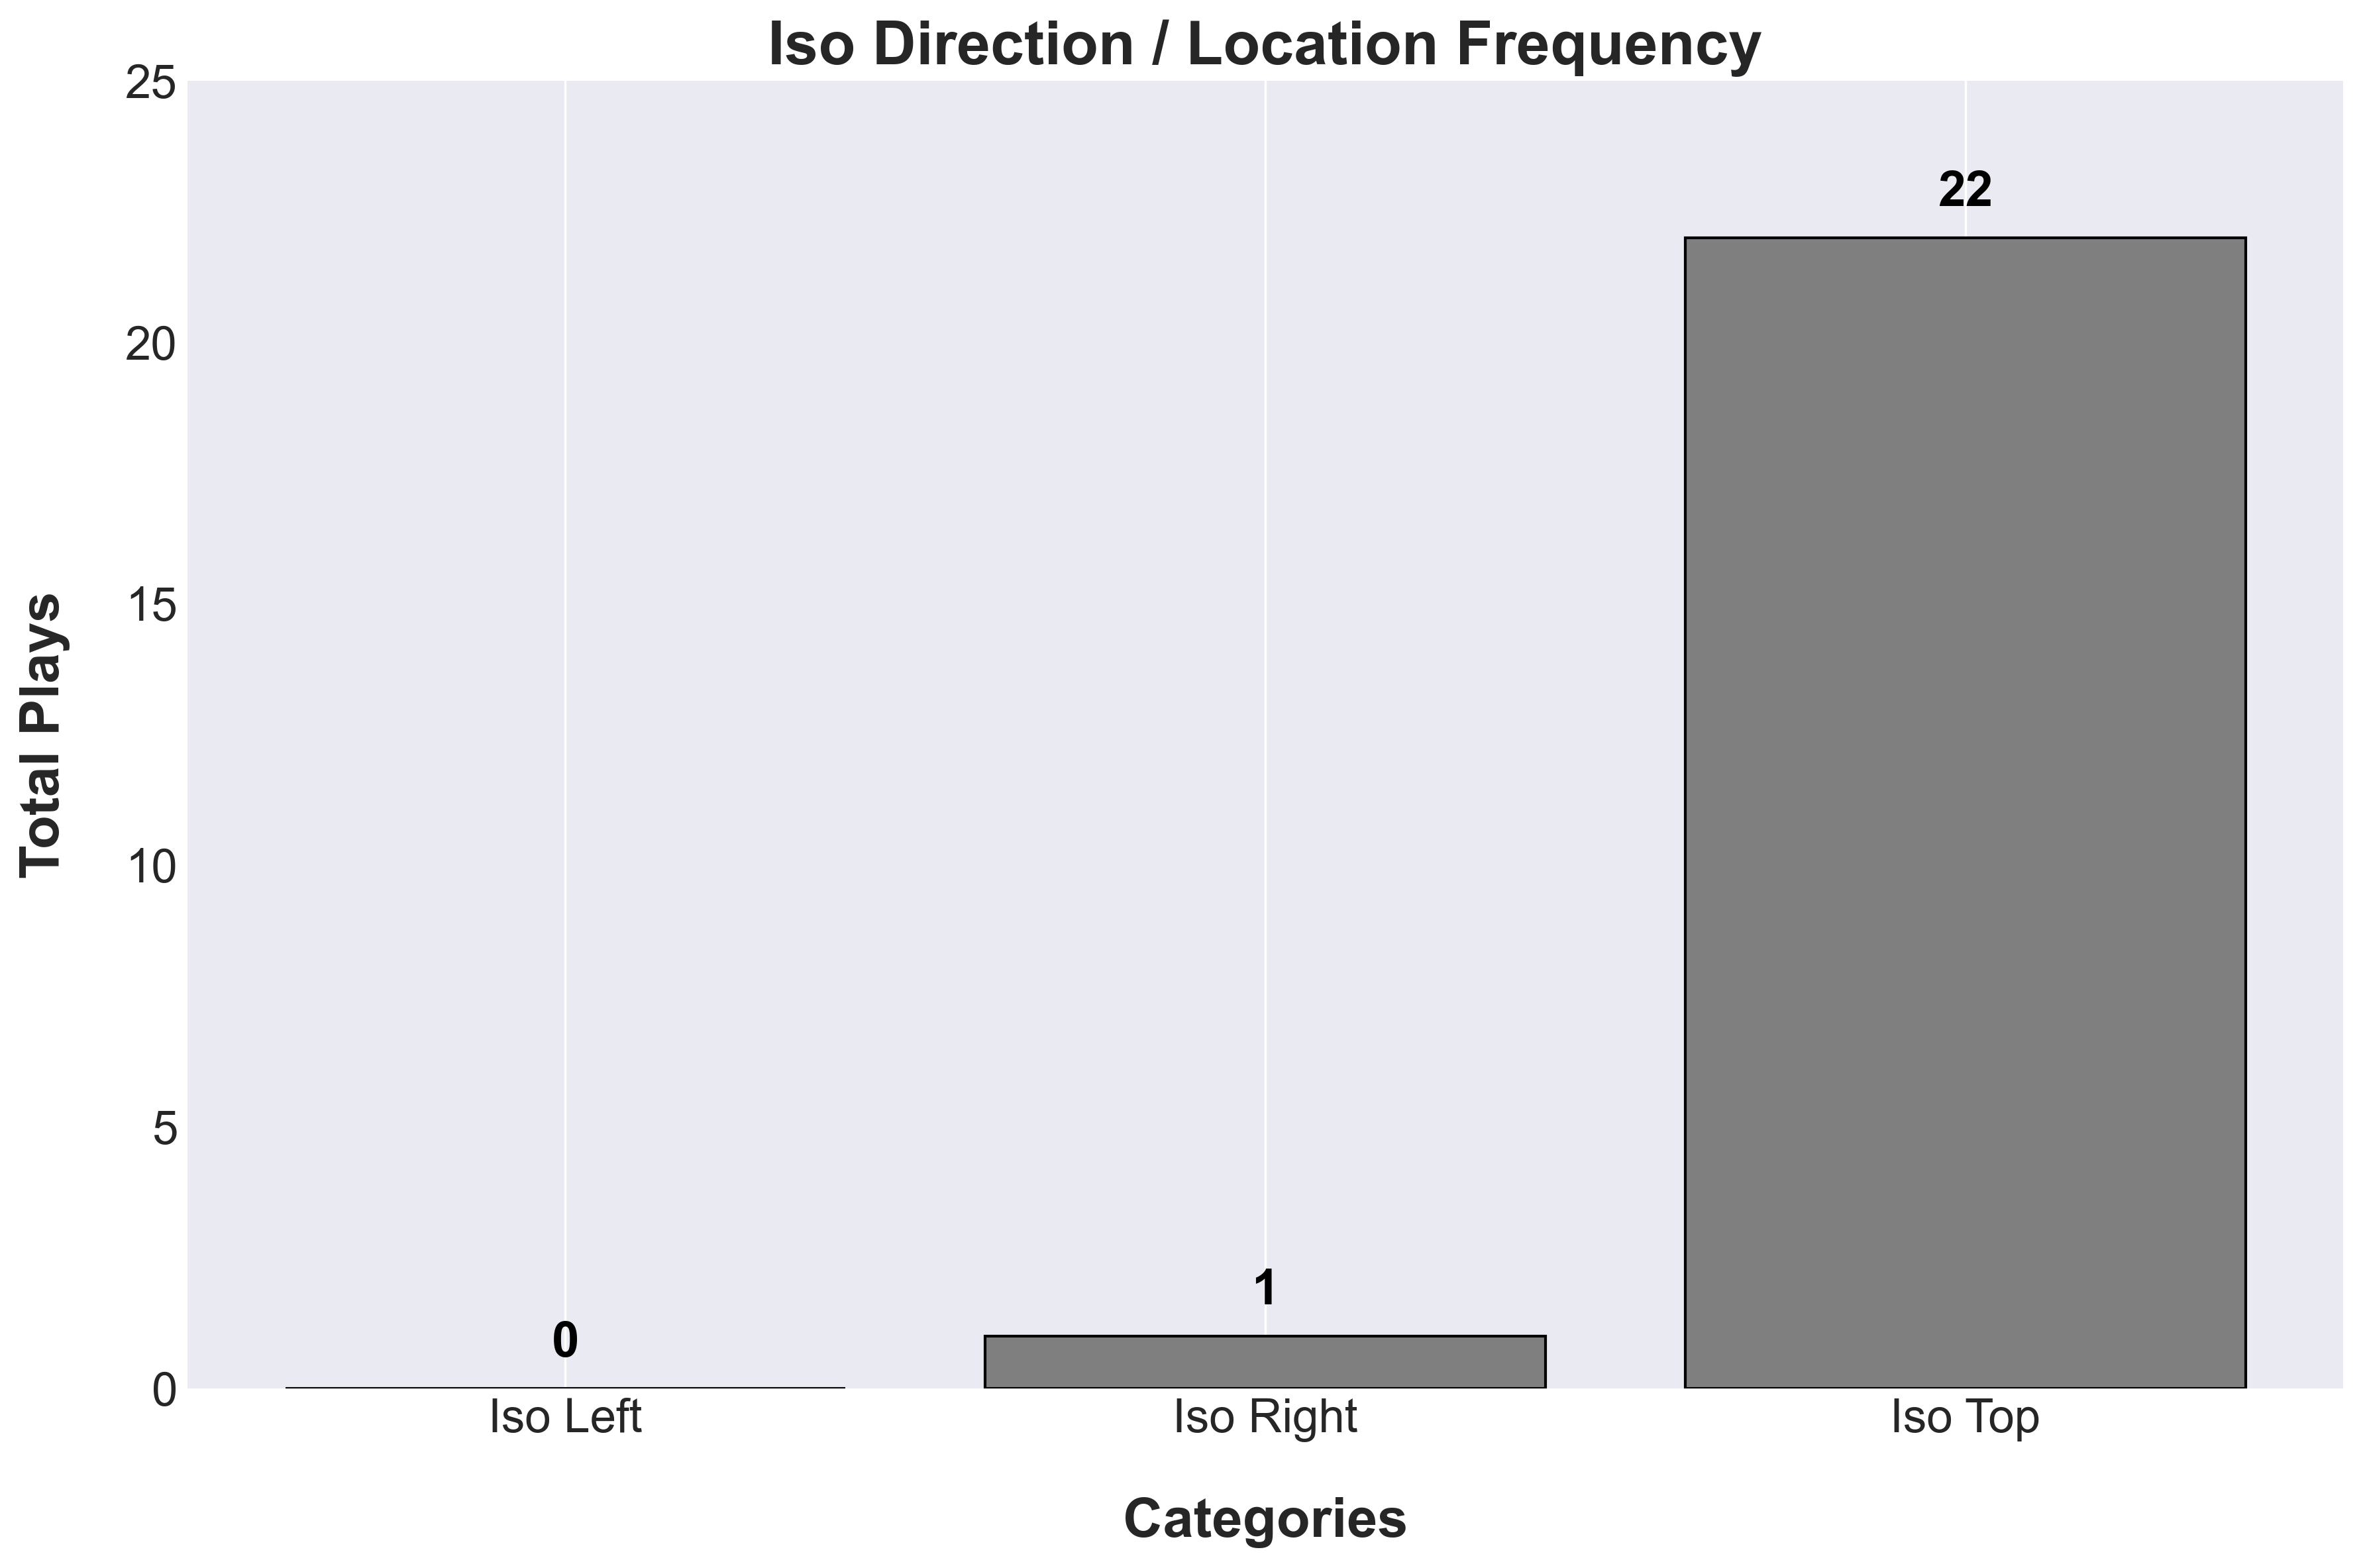
\includegraphics[width=\textwidth, height=.14\textheight]{images/IsoDirectionLocation_Freq.png} % Adjust the width of the image to fit
    \end{minipage}
\end{table}

\vspace{0em} % Add vertical space before the line (optional)
\hrule height 1pt width 1\textwidth % Adjust height and width
\vspace{1em} % Add vertical space after the line (optional)


% ----------------------
% Cutter Visuals and Insights Section
% ----------------------
\subsection{Cuts}

\vspace{1em} % Add vertical space after the line (optional)
\hrule height 1pt width 1\textwidth % Adjust height and width
\vspace{1em} % Add vertical space after the line (optional)

\subsubsection{General Cutter Stats}
% All Cutter Statistics Table w/ room for insights
\begin{table}[H]
    \centering
    \begin{minipage}[t]{0.6\textwidth} % Left side (table) takes 60% of the width
        \centering % Centering the title and the table
        \textbf{Total Cutter Statistics} % Title above the table in bold
        \vskip .25em % Adds vertical space between title and table
        \scalebox{.85}{ % Scale the entire table down by 85%
            \scriptsize % Reduce the font size
            \begin{tabular}{
            >{\centering\arraybackslash}p{.75cm} 
            >{\centering\arraybackslash}p{.5cm} 
            >{\centering\arraybackslash}p{.5cm} 
            >{\centering\arraybackslash}p{.5cm}
            >{\centering\arraybackslash}p{.5cm} 
            >{\centering\arraybackslash}p{.5cm} 
            >{\centering\arraybackslash}p{.5cm} 
            >{\centering\arraybackslash}p{.5cm}
            >{\centering\arraybackslash}p{.5cm} 
            >{\centering\arraybackslash}p{.5cm}
            >{\centering\arraybackslash}p{.5cm} 
            >{\centering\arraybackslash}p{.5cm}}% Adjust column widths
            \toprule
            \textbf{Plays} &
            \textbf{3PA} &
            \textbf{3PM} &
            \textbf{3P\%} & 
            \textbf{2PA} & 
            \textbf{2PM} & 
            \textbf{2P\%} & 
            \textbf{MiA} & 
            \textbf{MiM} &
            \textbf{Mi\%} &
            \textbf{TO} &
            \textbf{Foul} \\
            \midrule
            
                
            
                
            
                
            
                
            
                
            
                
                    58 & 0 &
                    0 & - & 
                    48 & 29 &
                    60.42 &
                    0 & 0 &
                    - &
                    4 & 6 \\ 
                
            
                
            
                
            
                
            
                
            
            \bottomrule
            \end{tabular}
        }
    \end{minipage}
\end{table}

\vspace{0em} % Add vertical space before the line (optional)
%\hrule height 1pt width 1\textwidth % Adjust height and width
\vspace{-1em} % Add vertical space after the line (optional)

% Cutter Stats for Basket vs Flash vs Screen Cuts 
\begin{table}[H]
    \raisebox{3em}{ % Adjust this value to shift the tables vertically
    \begin{minipage}[t]{0.6\textwidth} % Left side (table) takes 60% of the width
        \flushleft
        \centering % Centering the title and the table
        \textbf{Cut Type Statistics} % Title above the table in bold
        \vskip .25em % Adds vertical space between title and table
        \scalebox{.6}{ % Scale the entire table down by 60%
            \renewcommand{\arraystretch}{1.4} % Adjust the number to increase or decrease row spacing
            \begin{tabular}{
            >{\centering\arraybackslash}p{1.75cm} 
            >{\centering\arraybackslash}p{.75cm} 
            >{\centering\arraybackslash}p{.75cm} 
            >{\centering\arraybackslash}p{.75cm} 
            >{\centering\arraybackslash}p{.75cm}
            >{\centering\arraybackslash}p{.75cm} 
            >{\centering\arraybackslash}p{.75cm} 
            >{\centering\arraybackslash}p{.75cm} 
            >{\centering\arraybackslash}p{.75cm}
            >{\centering\arraybackslash}p{.75cm} 
            >{\centering\arraybackslash}p{.75cm}
            >{\centering\arraybackslash}p{.75cm} 
            >{\centering\arraybackslash}p{.75cm}}% Adjust column widths
            \toprule
            {\scriptsize \textbf{PlayType}} &
            {\scriptsize \textbf{Plays}} &
            {\scriptsize \textbf{3PA}} &
            {\scriptsize \textbf{3PM}} &
            {\scriptsize \textbf{3P\%}} & 
            {\scriptsize \textbf{2PA}} & 
            {\scriptsize \textbf{2PM}} & 
            {\scriptsize \textbf{2P\%}} & 
            {\scriptsize \textbf{MiA}} & 
            {\scriptsize \textbf{MiM}} &
            {\scriptsize \textbf{Mi\%}} &
            {\scriptsize \textbf{TO}} &
            {\scriptsize \textbf{Foul}} \\
            \midrule
            
                
            
                
            
                
            
                
            
                
            
                
            
                
            
                
                    Basket & 31 & 0 &
                    0 & - & 
                    25 & 15 &
                    60.0 &
                    0 & 0 &
                    - &
                    2 & 4 \\
                
            
                        
                    Flash & 5 & 0 &
                    0 & - & 
                    3 & 3 &
                    100.0 &
                    0 & 0 &
                    - &
                    1 & 1 \\
                
            
                 
                    Screen & 22 & 0 &
                    0 & - & 
                    20 & 11 &
                    55.0 &
                    0 & 0 &
                    - &
                    1 & 1 \\
                
            


            \bottomrule
        \end{tabular}
        } % End of \scalebox
    \end{minipage}
    } % End of raisebox, closing the adjustment
    \hfill % This adds some flexible space between the table and the image
    \begin{minipage}[c]{0.35\textwidth} % Right side (image) takes 35% of the width
        \flushright
        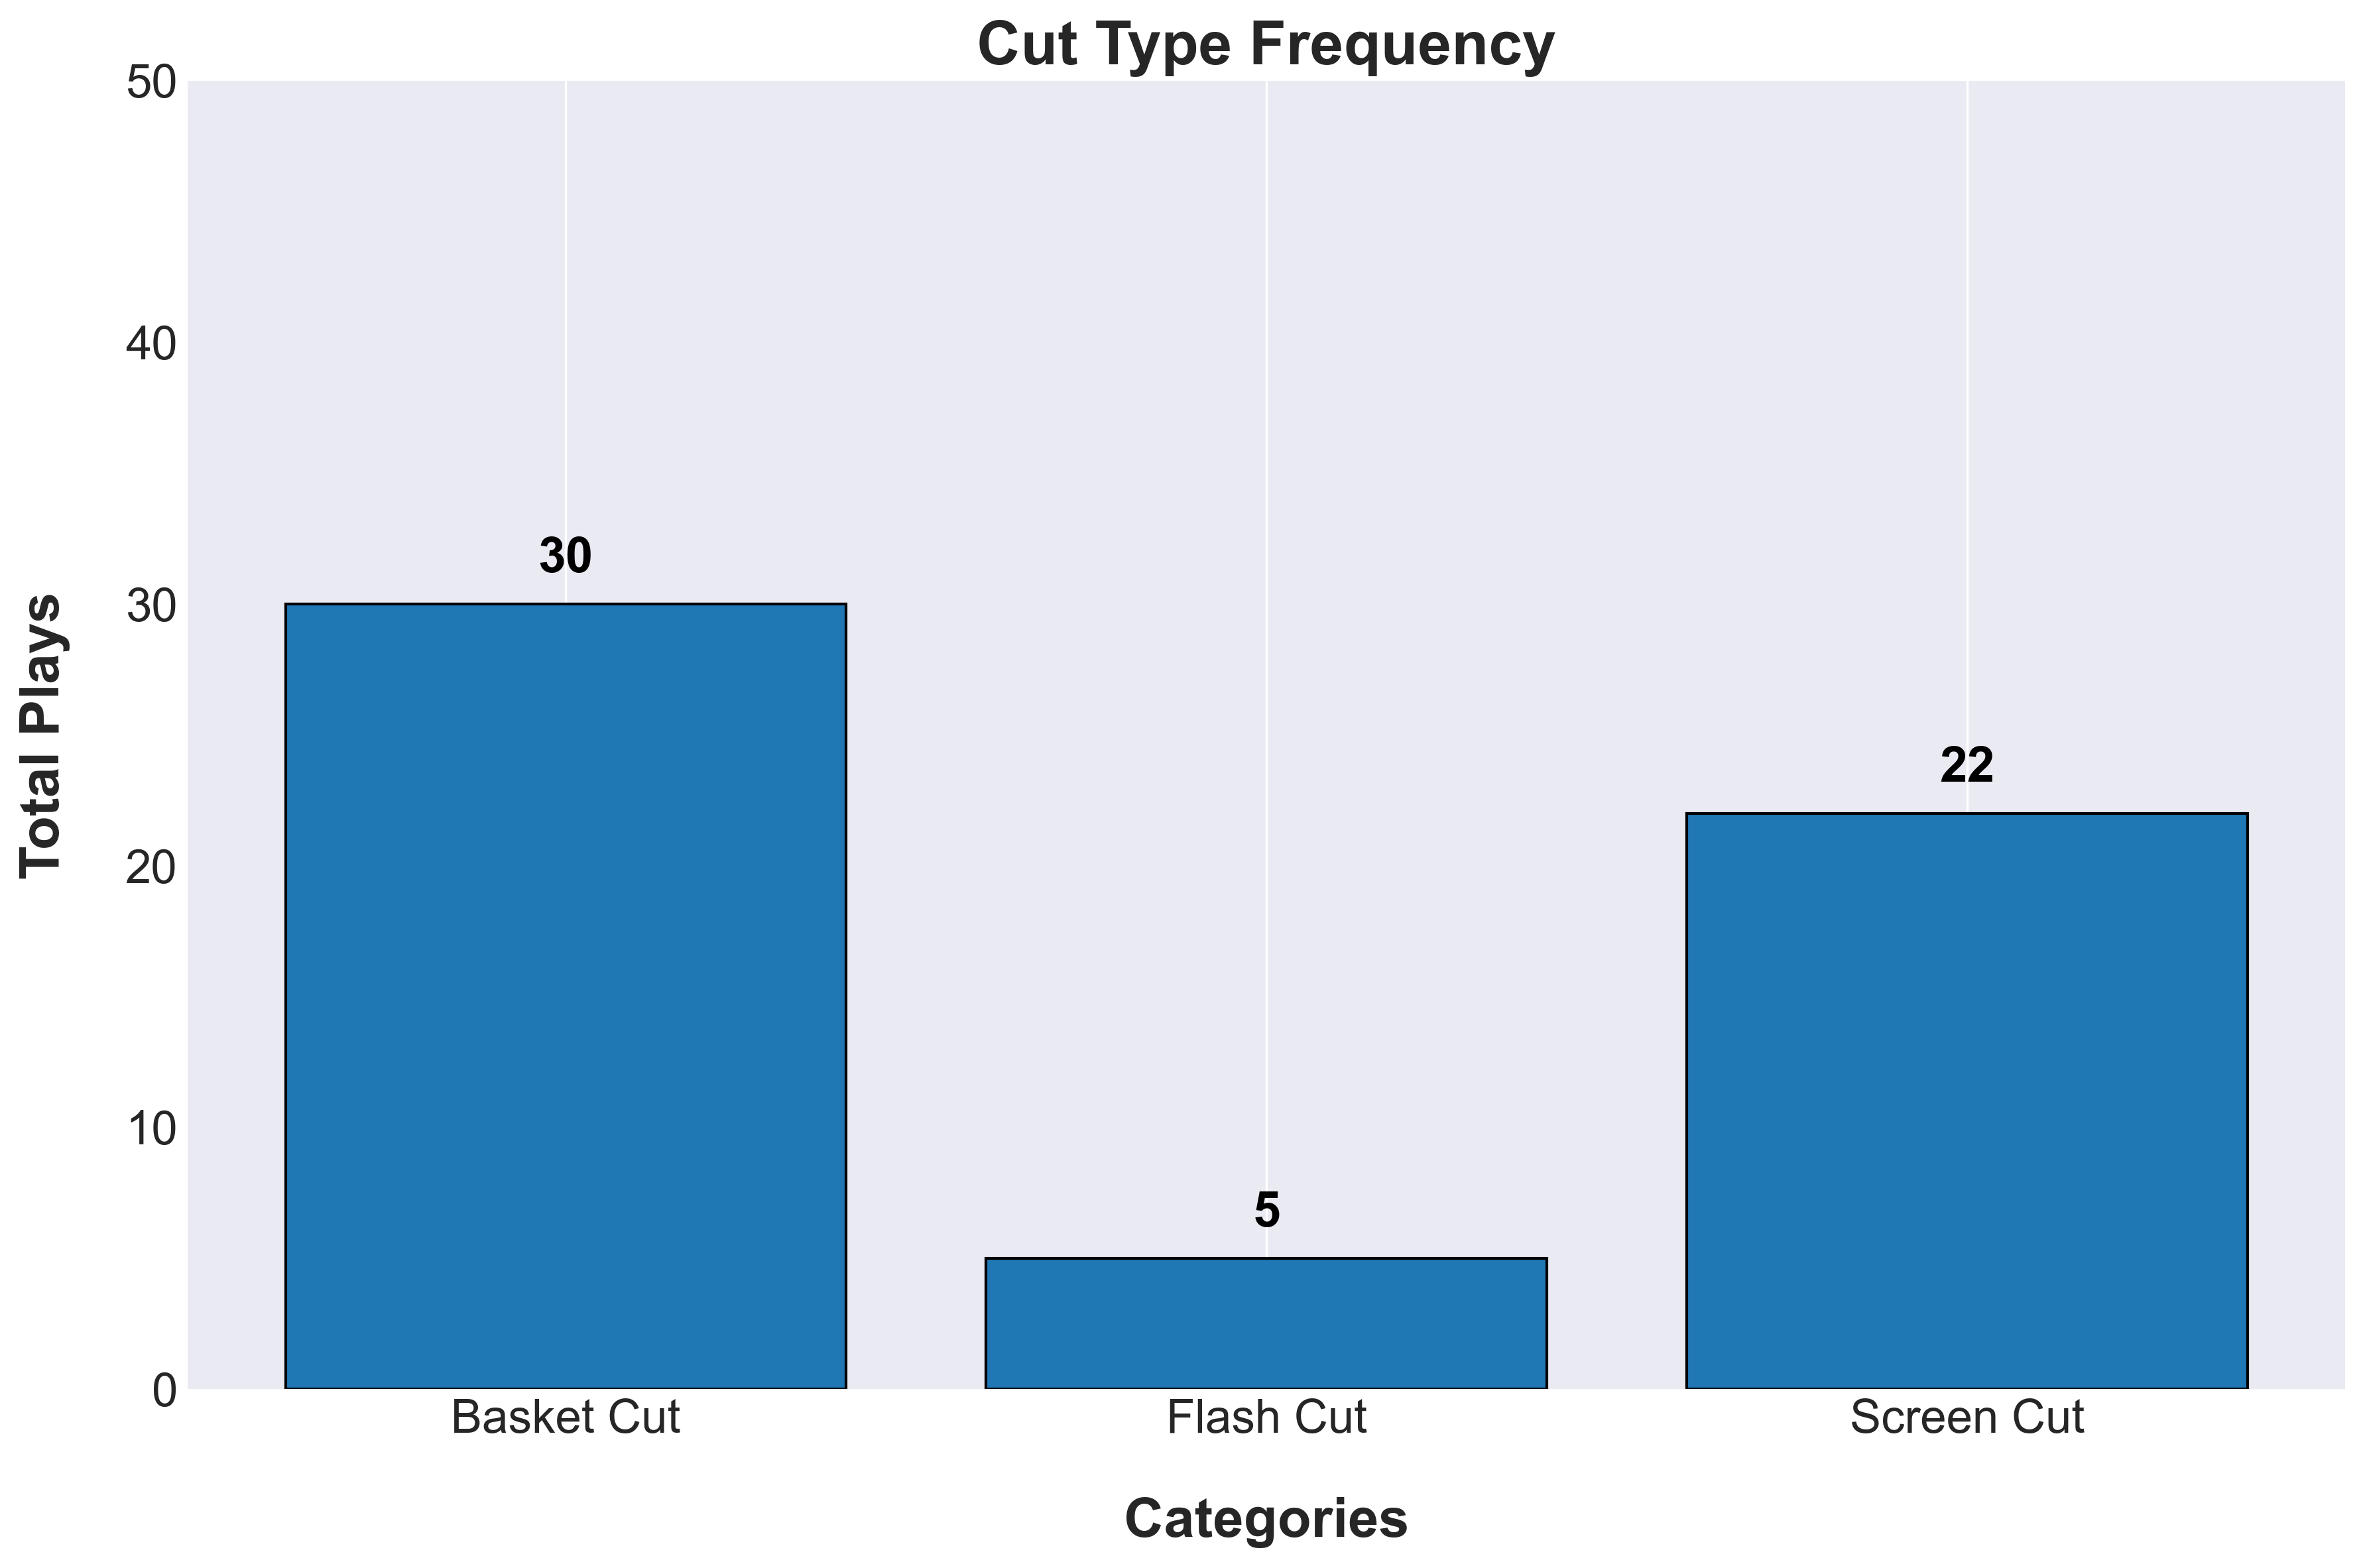
\includegraphics[width=\textwidth, height=.14\textheight]{images/Cut_Type_Freq.png} % Adjust the width of the image to fit
    \end{minipage}
\end{table}

\vspace{0em} % Add vertical space before the line (optional)
\hrule height 1pt width 1\textwidth % Adjust height and width
\vspace{1em} % Add vertical space after the line (optional)




% ----------------------
% Transition Visuals and Insights Section
% ----------------------
\subsection{Transition}

\vspace{1em} % Add vertical space after the line (optional)
\hrule height 1pt width 1\textwidth % Adjust height and width
\vspace{1em} % Add vertical space after the line (optional)

\subsubsection{General Transition Stats}
% All Cutter Statistics Table w/ room for insights
\begin{table}[H]
    \centering
    \begin{minipage}[t]{0.6\textwidth} % Left side (table) takes 85% of the width
        %\flushright
        \centering % Centering the title and the table
        \text{Total Transition Statistics} % Title above the table in bold
        \vskip .25em % Adds vertical space between title and table
        \scalebox{.85}{ % Scale the entire table down by half
            \scriptsize % Reduce the font size
            \begin{tabular}{
            >{\centering\arraybackslash}p{.75cm} 
            >{\centering\arraybackslash}p{.5cm} 
            >{\centering\arraybackslash}p{.5cm} 
            >{\centering\arraybackslash}p{.5cm}
            >{\centering\arraybackslash}p{.5cm} 
            >{\centering\arraybackslash}p{.5cm} 
            >{\centering\arraybackslash}p{.5cm} 
            >{\centering\arraybackslash}p{.5cm}
            >{\centering\arraybackslash}p{.5cm} 
            >{\centering\arraybackslash}p{.5cm}
            >{\centering\arraybackslash}p{.5cm} 
            >{\centering\arraybackslash}p{.5cm}}% Adjust column widths
            \toprule
            \textbf{Plays} &
            \textbf{3PA} &
            \textbf{3PM} &
            \textbf{3P\%} & 
            \textbf{2PA} & 
            \textbf{2PM} & 
            \textbf{2P\%} & 
            \textbf{MiA} & 
            \textbf{MiM} &
            \textbf{Mi\%} &
            \textbf{TO} &
            \textbf{Foul} \\
            \midrule
            
                
            
                
                    18 & 1 & 0 &
                    0.0 & 
                    14 & 12 &
                    85.71 &
                    2 & 2 &
                    100.0 &
                    1 & 2 \\
                
            
                
            
                
            
                
            
                
            
                
            


            \bottomrule
            \end{tabular}
        }
    \end{minipage}
\end{table}

\vspace{0em} % Add vertical space before the line (optional)
%\hrule height 1pt width 1\textwidth % Adjust height and width
\vspace{-1em} % Add vertical space after the line (optional)

% Transition Stats for BH vs Leakouts vs Left Wing vs Right Wing vs Trailer
\begin{table}[H]
    \raisebox{4.5em}{ % Adjust this value to shift the tables vertically
    \begin{minipage}[t]{0.6\textwidth} % Left side (table) takes 85% of the width
        \flushleft
        \centering % Centering the title and the table
        \text{Transition Type Statistics} % Title above the table in bold
        \vskip .25em % Adds vertical space between title and table
        \scalebox{.58}{ % Scale the entire table down by half
            \renewcommand{\arraystretch}{1.4} % Adjust the number to increase or decrease row spacing
            \begin{tabular}{
            >{\centering\arraybackslash}p{2.5cm} 
            >{\centering\arraybackslash}p{.75cm} 
            >{\centering\arraybackslash}p{.75cm} 
            >{\centering\arraybackslash}p{.75cm} 
            >{\centering\arraybackslash}p{.75cm}
            >{\centering\arraybackslash}p{.75cm} 
            >{\centering\arraybackslash}p{.75cm} 
            >{\centering\arraybackslash}p{.75cm} 
            >{\centering\arraybackslash}p{.75cm}
            >{\centering\arraybackslash}p{.75cm} 
            >{\centering\arraybackslash}p{.75cm}
            >{\centering\arraybackslash}p{.75cm}
            >{\centering\arraybackslash}p{.75cm}}% Adjust column widths
            \toprule
            {\scriptsize \textbf{PlayType}} &
            {\scriptsize \textbf{Plays}} &
            {\scriptsize \textbf{3PA}} &
            {\scriptsize \textbf{3PM}} &
            {\scriptsize \textbf{3P\%}} & 
            {\scriptsize \textbf{2PA}} & 
            {\scriptsize \textbf{2PM}} & 
            {\scriptsize \textbf{2P\%}} & 
            {\scriptsize \textbf{MiA}} & 
            {\scriptsize \textbf{MiM}} &
            {\scriptsize \textbf{Mi\%}} &
            {\scriptsize \textbf{TO}} &
            {\scriptsize \textbf{Foul}} \\
            \midrule
            
                
            
                
            
                
                    BH & 2 & 0 & 0 &
                    - & 
                    2 & 2 &
                    100.0 &
                    0 & 0 &
                     &
                    0 & 0 \\
                
            
                
                    Leakouts & 2 & 0 & 0 &
                    - & 
                    2 & 2 &
                    100.0 &
                    0 & 0 &
                    - &
                    0 & 0 \\
                
            
                
                    Left Wing & 2 & 0 & 0 &
                    - & 
                    2 & 1 &
                    50.0 &
                    0 & 0 &
                    - &
                    0 & 0 \\
                
            
                
                    Right Wing & 4 & 0 & 0 &
                    - & 
                    4 & 4 &
                    100.0 &
                    0 & 0 &
                    - &
                    0 & 0 \\
                
            
                
                    Trailer & 8 & 1 & 0 &
                    0.0 & 
                    4 & 3 &
                    75.0 &
                    2 & 2 &
                    100.0 &
                    1 & 2 \\
                
            


            \bottomrule
        \end{tabular}
        } % End of \scalebox
    \end{minipage}
    } % End of raisebox, closing the adjustment
    \hfill % This adds some flexible space between the table and the image
    \begin{minipage}[c]{0.35\textwidth} % Right side (image) takes 10% of the width
        \flushright
        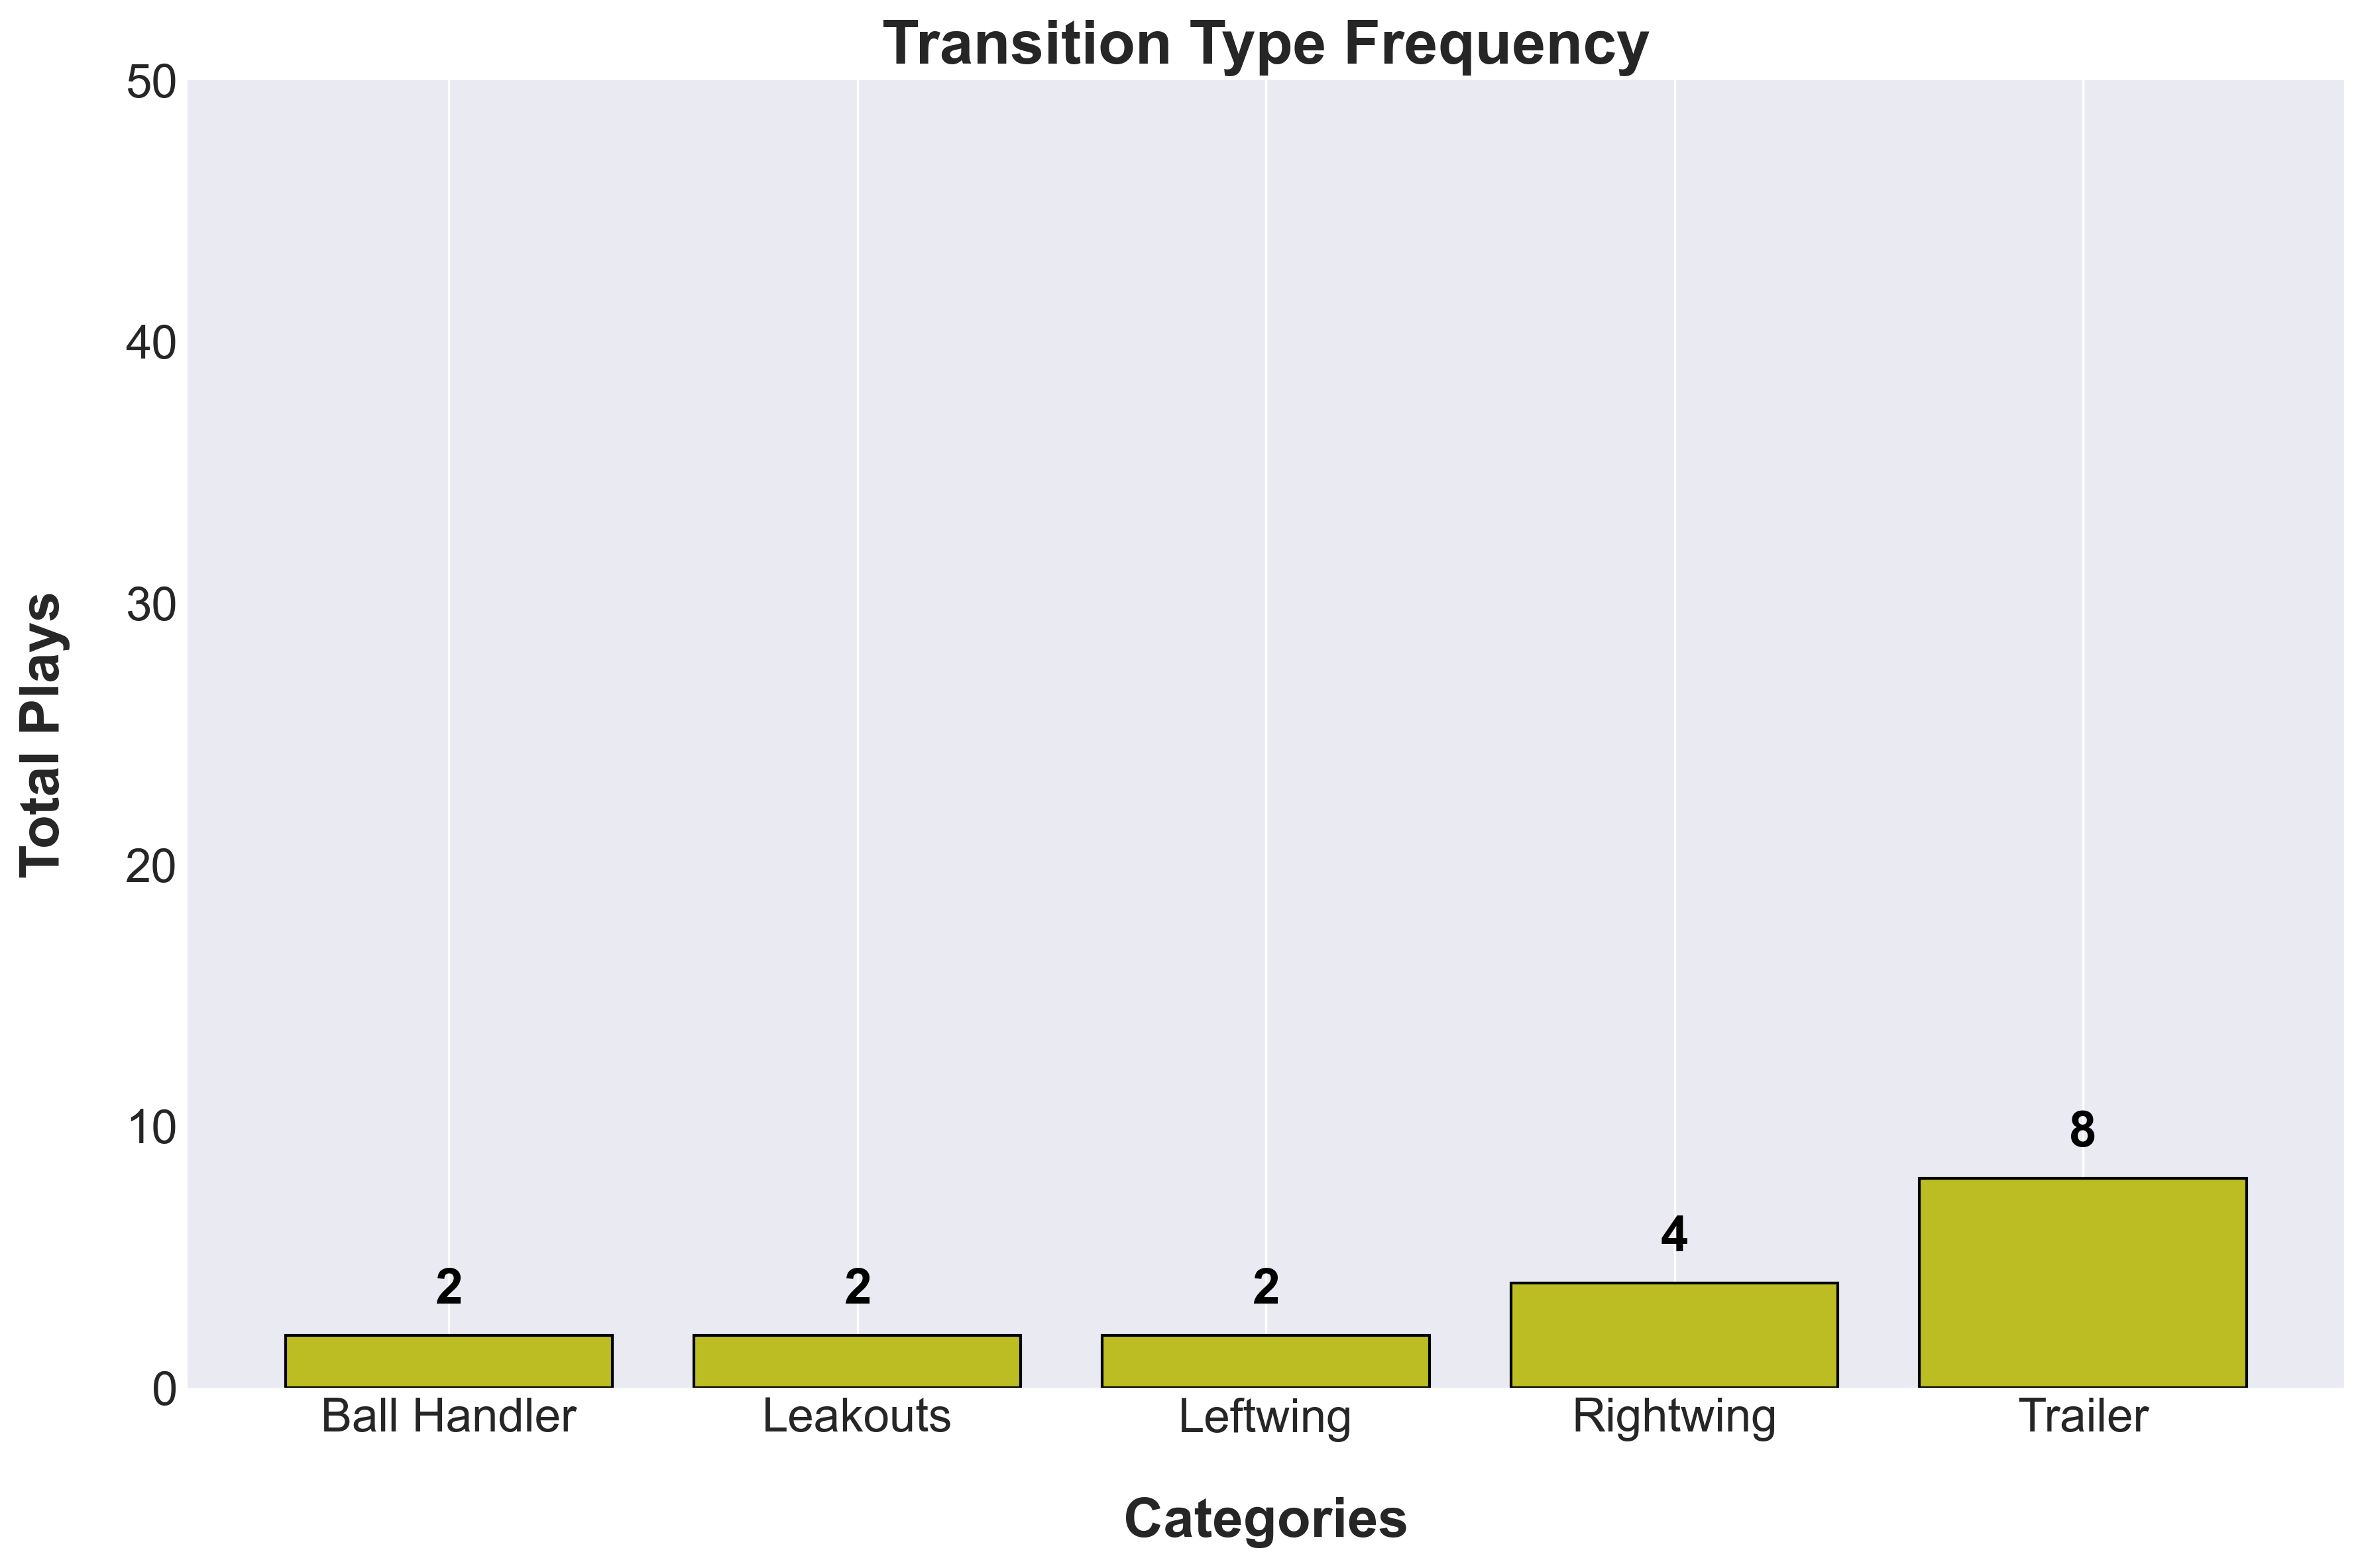
\includegraphics[width=\textwidth, height=.14\textheight]{images/Transition_Type_Freq.png} % Adjust the width of the image to fit
    \end{minipage}
\end{table}

\vspace{0em} % Add vertical space before the line (optional)
\hrule height 1pt width 1\textwidth % Adjust height and width
\vspace{1em} % Add vertical space after the line (optional)

\clearpage


%---------------------------------
% Data Disclaimers
%---------------------------------
\section*{Data Disclaimers}

\vspace{0.5cm} % Adds vertical space between items

\begin{itemize}[leftmargin=*, label=\textbf{•}]
    \item \textbf{Legal Data Collection:} All data presented in this document was legally scraped from Synergy using a program developed by Kyle Krebs.
    
    \vspace{0.3cm} % Adds vertical space between items

    \item \textbf{Purpose of Report:} This report aims to offer detailed insights into specific player statistics, facilitating players and coaches in comprehensively understanding the behavioral patterns of their opponents.

    \vspace{0.3cm} % Adds vertical space between items
    
    \item \textbf{Use of Report:} This report is intended to demonstrate my skills in data analysis and report generation. Please note that all personal names and team names have been anonymized to protect privacy and maintain confidentiality when showing 3rd parties.
    
    \vspace{0.3cm}
    
    \item \textbf{Data Accuracy:} While efforts have been made to ensure the accuracy of the data, there may still be some errors in the numbers. If you identify any discrepancies, please feel free to reach out to me.
    
    \vspace{0.3cm}
    
    \item \textbf{Permission Granted:} I have received permission from coaches to use and analyze data that has been scraped from Synergy.
    
    \vspace{0.3cm}
    
    \item \textbf{Content Generation:} All content generated in the following report was created by Kyle Krebs.
\end{itemize}

\vspace{0cm} % Adds space before the contact section

\subsubsection*{Contact Information}

For questions or concerns regarding this report or data privacy, please contact:

\begin{itemize}[leftmargin=*, label={}]
    \item \textbf{Kyle Krebs}
    \item \textbf{Email:} \href{mailto:kak4294@rit.edu}{kak4294@rit.edu}
    \item \textbf{Phone:} 845-418-9959
\end{itemize}


\vspace{1.5em}

\small
\section*{General Stat Information \& Statistic Definitions}

    \vspace{1em}
    \noindent \textbf{!! IMPORTANT PLEASE READ !!} All statistics measured in this report were actions that had ended in either a shot taken, foul drawn, or turnover. With this information we are able to intrepet where players get their shots from. This doesn't track total amount of times a player does a specific action, it only tracks when those actions end in the way I said above. 
    \vspace{1em}
    
    \noindent \textbf{Offensive Load:} Measures the total number of offensive actions a player performs, including shots taken, fouls drawn, and turnovers.
    
    \noindent \textbf{Efficiency:} Measured by a players performance of their 3pt\%, 2pt\%, Midrange\%, Turnovers, and Fouls Drawn

\vspace{.3em}


    
\subsection*{Pick-and-Roll}

    \noindent \textbf{Usage:} Determines whether a player goes off a screen or rejects it.
    
    \noindent \textbf{Direction/Location:} Direction pertains to the stats in the 'Left' / 'Right' rows as they give us the direction the ball handler is going. Location pertains to the stats in the 'High' row as it tells us the screen occurs when the screener is completely outside the 3 point line. Direction is unknown in High pick-and-rolls.
    
    \noindent \textbf{PNR to Different Playtypes:} Each row pertains to another action to which the ball handler had passed it to another player out of the pick-and-roll that proceeded to execute the given action.

\vspace{.5em}

\subsection*{Post Ups}

    \noindent \textbf{Location:} Pertains to the spot of the floor where the player had started his post up. 
    
    \noindent \textbf{Shot Type:} Tells us which shoulder the player had shot over, or if the player faced up on the post up. 
    
    \noindent \textbf{Post to Different Playtypes:} Each table pertains to another action to which the post player had passed it to another player out of the post that proceeded to execute the given action.

\vspace{.5em}

\subsection*{Rollman}

    \noindent \textbf{Play Type:} Represents whether the Rollman popped, slipped, or rolled to basket after screen.
    
    \noindent \textbf{Slip to Drive:} Goes over direction that player drove after slipping a screen and driving

     \noindent \textbf{Pop to Drive:} Goes over direction that player drove after popping and driving

\vspace{.5em}


\subsection*{Spot Ups}

    \noindent \textbf{Jumpshots:} Defined as a catch and shoot jump shot received from a pass of a teammate. 
    
    \noindent \textbf{Drives:} Defined as when someone catches the ball on the outside of the 3 point line and took at least one dribble to get a shot/turnover of some sort.
    
    \noindent \textbf{Drive Direction:} Defined as the which way the player had dribbled the ball after catching the pass in a spot up position.
    
    \noindent \textbf{Different Playtype to Jumpshot/Drive:} Pertains to an action that a player in a spot up position receives a pass from. 

\vspace{.5em}

\subsection*{Off Screens}

    \noindent \textbf{Running off Specific Shoulder:} Refers to the shoulder that the shooter hits the screener with when running off a screen. 
    
    \noindent \textbf{Type:} Refers to one of three options, \underline{Flare}: when someone sets a screen away from the player with the ball to help a teammate get open for a shot or move. \underline{Curl}: when a player comes off a screen and catches the ball going directly to the basket. \underline{Straight}: when a player runs directly off a screen to catch the ball at the three point line. 

\vspace{.5em}


\subsection*{Handoffs}

    \noindent \textbf{Direction/Location:} Direction refers to 'Left' / 'Right' rows, where the shooter receives the hand offs moving in the given direction. Location refers to the 'Top' row where direction is not specified, yet the location of the hand off happens at the center of the court above the 3 point line. 
    
    \noindent \textbf{Type:} Refers to what the person handing the ball off is doing when the shooter receives the hand off. \underline{Stationary}: staying in one spot. \underline{Dribble}: continuously dribbling towards shooter in hand off.

\vspace{.5em}

\subsection*{Iso}

    \noindent \textbf{Location:} Refers to where on the court the isolation occurs. \underline{Left} refers to left wing and left corner. \underline{Right} refers to right wing and right corner. \underline{Top} refers to center of the court above the three point line.

\vspace{.5em}

\subsection*{Cuts}

    \noindent \textbf{Type:} Refers to one of three options. \underline{Basket}: when a player gets a pass running towards the basket. \underline{Flash}: when a player catches a pass running towards an open space on the court. \underline{Screen}: when a player receives a pass running off a screen to which he runs towards the basket. 
    
\vspace{.5em}

\subsection*{Transition}

    \noindent \textbf{Type:} \underline{BH} refers to Ball Handler, where a player gets the ball in transition and dribbles down the court leading them to get themselves a shot or turn the ball over. \underline{Leakouts} refer to a player running up the court ahead of the ball receiving a pass and getting a shot/turnover. \underline{Left Wing} refers to a player getting a pass at the left side of the court in transition leading to a score/turnover. \underline{Right Wing} refers to a player getting a pass at the right side of the court in transition leading to a score/turnover. \underline{Trailer} refers to a player running up the court behind the ball where he receives a pass from a player in front of them with the ball. 

\clearpage


\end{document}